\documentclass[12pt, oneside]{extbook} % the document type needs to be change
\usepackage{geometry}
\usepackage{listings}
\usepackage{graphicx}

\geometry{
	a4paper,
	left = 1.5 cm,
	right = 1.5 cm,
	top = 2cm,
}

\title{Network and System Defense}

\begin{document}
\maketitle
\tableofcontents
\newpage
\part{Parte Hardware}
\chapter{Introduzione}
In cybersecurity, ci sono almeno 5 aree esterne differenti che si mischiano fra loro, e poi 3 aree interne relative all'hardware ed al software.\\ "L'attore principale" sono applicazioni Internet-based:
\begin{itemize}
\item vulnerabilità del sistema, della rete etc
\item come difendersi o evitare tali vulnerabilità, o almeno mitigarle
\end{itemize}
Molta configurazione pratica: laboratori da 0, ma è utile rifare tutto a casa (\textbf{CAZZI}).\\ Per via del fatto che è davvero difficile oggi separare cosa è la rete da cosa è il software, è utile parlare di tutti i diversi campi che riguardano sia la rete che il software.\\ Punti chiave:
\begin{itemize}
\item Access networks and perimetral security: Ethernet, VLAN, IPv6, 802.11x, firewall, packet classification algorithms
\item Core networks: BGP, MPLS, DDos e Botnets, VPNs con BGP
\item End to End security: PKIs, DNS security, HTTPS, Overlay VPNs
\item Sw and Operating System
\item Virtualization \& Cloud 
\end{itemize}
Piattaforme da utilizzare per la parte da 6 CFU (Hardware):
\begin{itemize}
\item GNS3
\item Tinycore Linux
\item VMware o Virtual Box: Virtual Box sembra lavorare meglio con GNS3
\item Cumulus Linux: serve per emulare le funzionalità di livello 2 di uno switch. Net OS, \textbf{scaricare la versione 4.1} e non le ultime. C'è un insieme di VM pronte per essere installate su un virtualizzatore
\item Immagini CISCO (da cercare online, if you know what I mean)
\item Lubuntu
\item Ubuntu server
\end{itemize}
\chapter{Introduzione alla cybersecurity}
Ci sono 3 fattori principali quando si parla di cyberscurity:
\begin{itemize}
\item Cosa bisogna proteggere?
\item Da quali minacce? Ci sono diverse fonti di attacco da cui proteggersi
\item Come fare per contrastare queste minacce? Integrità, encryption, etc...
\end{itemize}
\paragraph{Definizione di computer security:}le misure ed i controlli che garantiscono confidenzialità, integrità e disponibilità degli assets dei sistemi informativi, incluso hardware, software etc...
\begin{itemize}
\item confidenzialità: i dati sono privati, le informazioni confidenziali non sono note ad entità non autorizzate. Esempi: usare SSH o HTTPS per scambiare credenziali con un server.
\item Privacy: (slides)
\item Integrità: se dei dati, indica che essi sono cambiati solo in maniera autorizzata. Se voglio traferire un messaggio con cui trasferisco del denaro, non voglio che il contenuto sia compromesso. Se si parla di integrità dei sistemi, si intende che il sistema performi come deve (vedi slides)
\item disponibilità: si assicura che il sistema lavori in maniera corretta e che i servizi non siano negati ad utenti autorizzati
\end{itemize}
Altri aspetti importanti:
\begin{itemize}
\item Authenticity: dell'utente, indica che sia possibile verificare che l'utente è chi dice di essere. Della sorgente: capacità di verificare che un messaggio arriva da una sorgente effettivamente affidabile.
\item altri ... (slides)
\end{itemize} 
\textbf{ALTRE IMPORTANTI DEFINIZIONI CHE SI TROVANO SULLE SLIDES}. \\ Quali sono le diverse superfici di attacco:
\begin{enumerate}
\item la rete stessa: i sistemi sono Internet-based, quindi è sempre possibile attaccare la rete. Attaccare la rete implica sfruttare vulnerabilità della rete Internet: ARP, WEP, link fisici, intrusioni nella rete etc...
\item attacchi al software: vulnerabilità nell OS, server web, code injection etc...
\item attacchi all'umano: molte vulnerabilità create da noi stessi, social engineering, errori umani, mancanza di competenze etc...
\end{enumerate}
È importante non pensare che la sicurezza sia data solo dalla tecnologia, ma anche dalle persone.\\ \paragraph{CIS critical security controls:} 20 applicazioni pratiche che la SANS suggerisce di applicare per verificare la sicurezza di una corporation (anche piccola Enterprise). Ogni controllo ha dei sotto-controlli più "concreti"\\ Quindi, non avendo il tempo di fare tutto, ci concentrare su alcuni aspetti fondamentali di tutto l'insieme visto.
\section{Lezione 2: vulnerabilità intrinseche IP/TCP}
Prima di capire le vulnerabilità, è necessaria una revisione dei protocolli di rete.
\subsection{Architettura di IP}
Intenet non è altro che una inter-connessione di reti che possono avere differenti tecnologie.\\ La comunicazione fra i device è possibile con IP, che è implementato sui livelli 1 e 2 (che sono indipendenti). Ogni dispositivo è identificato dall'indirizzo univoco a 32/64 bit (che seguono la nomenclatura CIDR), le diverse sotto-reti comunicano tramite i router ovvero un device IP che ha almeno 3 livelli dello stack Internet. Ha diverse interfacce che possono essere in diverse tecnologie: ADSL, Ethernet, Fibra etc...\\ Le operazioni compiute dai router:
\begin{itemize}
\item IP forwarding: longest prefix mathcing, manda un pacchetto verso la prossima interfaccia del percorso di rete. È diretta se la destinazione è nella subnet, mentre indiretta se serve trovare il next hop, quindi andare fuori dalla propria sotto-rete. Il next hop è un dispositivo nella propria sotto-rete che sa come arrivare alla destinazione.
\end{itemize}
Il goal di IP è quello di mandare il pacchetto a destinazione, l'Internet è diviso in Autonomous Systems all'interno dei quali si può configurare il routing come si vuole. Ma poi, serve scambiare informazioni fra As, si parla quindi di protocolli intra-AS come OSPF, RIP e protocolli inter-AS, come BGP.\\ C'è l'header per ogni pacchetto che ha i diversi campi (TTL, src, dest, protocol, checksum etc...), diverso fra IPv4 ed IPv6, differenze fra i due:
\begin{itemize}
\item header più piccolo in IPv6
\item no fragmentation in IPv6
\end{itemize}
\paragraph{Routing table:}struttura dati che associa una destinazione ad un next hop. Per il routing si usa il longest prefix matching, l'IP più "specifico" è quello scelto. La differenza principale fra host e router è che se un host riceve un pacchetto da una src non fra quelle locali, lo scarta; un router lo forwarda. Il forwarding standard basico è fatto in base all'indirizzo di destinazione. Dopo l'estrazione del pacchetto IP, se l'IP dest è locale, lo manda al livello superiore, altrimenti lo guarda nella tabella di routing: se non si trova un matching, il pacchetto è scartato. Altrimenti: se c'è un next hop, bisogna scoprire chi è, altrimenti basta scoprire il MAC associato all'IP.\\ La maggior parte dei pacchetti che vengono mandati vanno fuori dall'AS con cui si firma il contratto: possono esserci diversi AS di transito prima di arrivare al data center del sito a cui si cerca di connettersi.
\subsection{Vulnerabilità di TCP/IP}
Per design, IP e TCP non si preoccupano della sicurezza in quanto sono stati progettati quando la sicurezza non era un problema. C'è un certo numero di vulnerabilità intrinseche nei protocolli, ed è ancora così in quanto sono stati progettati senza pensare all'aspetto di sicurezza:
\begin{itemize}
\item Identification: i device della rete possono essere falsificati, è possibile spoofare l'IP address per dire di essere , ad esempio, un certo server web. Sia per i pacchetti generati dall'utente che per quelli forwardati. Se mandiamo un pacchetto di un legittimo server DNS, stiamo impersonificando il server stesso. Non ci sono meccanismi in IP per verificare l'autenticità di chi manda il pacchetto
\item Reputation: come è possibile verificare che l'origine del pacchetto è effettivamente la sorgente?
\item Confidentiality: non vogliamo che le informazioni scambiate sulla rete siano viste da 3e parti. Vorrei che solo il server veda i dati in uno scambio client-server. Ma intercettare il pacchetto in maniera "malevola" è fattibile ed anche decodificarlo perché l'header e l'IP sono in chiaro.\\ Il problema non è nella rete interna, ma passa per diversi AS (noi ci fidiamo solo del nostro): anche se il path fra sorgente e destinazione è fidato, è possibile fare hijaking su BGP, fra gli attacchi più pericolosi e in voga.
\item Integrity: voglio essere sicuro che il pacchetto non sia modificato durante il percorso fra src e dest. C'è il checksum, ma è calcolato su dati in chiaro, quindi non va bene come "codice" per poter assicurare l'integrità
\item Packet replication: non c'è sequence number nell'IP header nella sessione, non ci sono meccanismi per proteggersi da questo threat
\end{itemize}
\subsubsection{Dynamic mapping}
Le cose si complicano perché i protocolli Internet usano diversi meccanismi per implementare il mapping: ad esempio il DSN, ARP, 802.3 bridging (lo switch impara in automatico quale MAC è dietro quale porta) e questo è dinamico in quanto può cambiare nel tempo. Questo problema è presente in ogni layer ed anche questi meccanismi non sono stati penasti per essere sicuri.
\paragraph{DNS spoofing:}possiamo spoofare una richiesta DNS, quindi fare un hijack della sessione. Attacco triviale (e vecchio):
\begin{itemize}
\item sfruttiamo il mapping MAC-IP per diventare MiTM
\item sfruttiamo il mapping fra il nome di dominio e l'IP per impersonare il server web
\item mappiamo l'IP del sito al nostro
\end{itemize}
Lo scenario è che l'attaccante sia nella stessa sotto-rete.\\ L'idea è quella di mandare dei messaggi ARP spoofati per far credere alla vittima di essere il default gateway e di fra credere al default gateway di essere la vittima.\\ Per impersonare il sito target è possibile usare il comando \textsf{wget}, ed usare Apache2 per impersonare il server web.\\ L'attacco sfrutta 3 vulnerabilità:
\begin{itemize}
\item ARP spoofing
\item DNS redirection
\item Impersonification
\end{itemize}
Per emulare un server DNS è possibile configurare bind ma c'è un piccolo servizio DNS da configurare e che permette di forwardare all'attacker tutto ciò che sono è noto.
\subsection{Security requirements per le vulnerabilità}
Vediamo cosa è possibile risolvere questi problemi: per la confidenzialità si usano algoritmi a chiave simmetrica per garantirla.\\ Un algoritmo a chiave simmetrica, entrambe le end della comunicazione condividono la stessa chiave, c'è anche la differenza fra:
\begin{itemize}
\item stream ciphers 
\item block ciphers, che usano concatenazione per evitare ECB, in cui se la stessa chiave viene riusata per molto è possibile scoprire il contenuto di blocchi che hanno lo stesso contenuto
\end{itemize}
Per l'integrità, vogliamo una prova che nessuno modifichi il contenuto del messaggio, quindi si produce un MAC basato su hash functions: l'hash è calcolato non solo sui dati ma anche sulla chiave.\\ L'Authenticated Encryption permette, con "la stessa chiave" di fornire sia confidenzialità che integrità. Si può ottenere un algoritmo del genere anche con le tecniche base di symmetric encyption.\\ Per l'autenticità è possibile usare pub key cryptography per realizzare dei meccanismi di firma, come RSA e Diffie-Hellman. Serve comunque avere una certificazione che un utente è il vero proprietario di una chiave, quindi che sia crittograficamente legato alla chiave: Public Key Infrastructure.
\section{Lezione 3: Ethernet LAN security}
Ethernet è una tecnologia di livello 2, il primo standard open e multi-vendor nato nel 1976.\\ L'802 è una famiglia di standard dell'IEEE, fra di essi ci sono diversi gruppi di lavoro e quello che si occupa di Ethernet è 802.3 e quindi si parla di questi standard, in quanto Ethernet era il nome commerciale.\\ La trama Ethernet originale ha un header molto snello, c'è il campo type / length che può essere due campi differenti a seconda della situazione (vedi slides)\\ Anche in questo caso è tutto in chiaro, quindi ci sono gli stessi problemi. Gli indirizzi MAC sono a 48 bit
\paragraph{Hub, Switch e Bridge:} un hub è uno strumento che forwarda pacchetti verso tutti. Uno switch ha un forwading database, ovvero una struttura dati che associa MAC alle porte. Lo switch impara in automatico quale è il MAC dietro una certa porta. Il problema sta proprio nel fatto che lo switch impara in automatico il mapping.\\ Si usa l'algoritmo spanning three per evitare i loop, che si possono creare perché, per motivi di ridondanza, è possibile avere dei loop nella rete.\\\\ Per operare al di sopra di Ethernet, IPv4 usa ARP e DHCP mentre IPv6 usa NDP, protocollo simile. NDP non è sicuro, ma c'è un protocollo per renderlo sicuro e lo stesso protocollo è stato progettato già pensando alla sicurezza.\\ Anche nel caso di DHCP, usato per ottenere un IP, abbiamo gli stessi problemi detti sopra.
\subsection{Ethernet LAN vulnerabilities}
Quali sono le possibili contro-misure per difendersi dai threats. I problemi di Ethernet sono dovuti al fatto che per natura si auto.configura. Siccome è possibile avere accesso a qualunque trama Ethernet, l'attaccante può:
\begin{itemize}
\item imparare qualcosa sulla topologia della rete
\item avere accesso agli switch
\item eavesdropping
\item etc...
\end{itemize}
Vediamo alcune categorie di problemi
\subsubsection{Network and system access}
Come è possibile ottenere accesso ad un Ethernet segment: unioni non autorizzate:
\begin{itemize}
\item tramite accesso fisico allo switch, se la porta è attiva
\item accedere ad una socket a muro
\item rimuovere il cavo ad un PC e metterlo in un altro
\item inserire uno switch fra il PC esistente e la socket
\end{itemize}
Espansioni della rete non autorizzate.\\ Un altro modo per ottenere l'accesso è quello di accedere in maniera remota, o anche fare il probe della rete per scoprire informazioni, come ad esempio usare nmap. Altri modi:
\begin{itemize}
\item break-ins
\item switch control: uno switch che ha password di default o non la ha e la password può essere resettata fisicamente. Se si ottiene il controllo di uno switch si possono fare varie cose, ad esempio se lo switch gira su cumulus Linux
\end{itemize}
Una volta che si è ottenuto l'accesso alla rete, si può fare lo sniffing del traffico di rete. Oggi non è più vero che la trama arriva a tutti e che sono tutti connessi, se la possibilità di intercettare fisicamente il pacchetto, è possibile fare un MiTM etc...\\ Ma il problema è anche nella procedura di learning dello switch: il MAC non è autenticato, quindi mandando una trama con un MAC reale allo swtich, viene ingannato nel pensare che il MAC è dietro una porta sbagliata.\\ Quindi l'attaccante può redirigere il traffico trasmesso dalla vittima verso se stesso, anche se è più che altro teorico perché anche la vittima manda messaggi.\\ Si può generare un pacchetto con un indirizzo falso, o anche intercettare un pacchetto e cambiarlo in quanto anche a livello 2 non c'è integrity check o HMAC tag.\\ Per cambiare il MAC, ci sono vari modi:
\begin{itemize}
\item cambiare il MAC della NIC (comando Linux)
\item usare raw socket programming
\item in-kernel programming
\end{itemize}
Per intercettare il pacchetto, basta mettere l'interfaccia di rete in modalità promiscua per ricevere tutto il traffico anche non diretto a me, così da poter cambiare il MAC.
\paragraph{MAC flooding:}l'idea è di inondare lo switch con un grande numero di trame con diversi indirizzi MAC per saturare la memoria dello switch in modo da far si che tutti i pacchetti siano inviati verso tutte le porte in broadcast.\\
\paragraph{ARP e DHCP poisoning:}si può fare ARP poisoning (vedi sopra) ma anche facendo poisoning di DHCP facendo creder di essere il server, spoofando tutto lo scambio DHCP.\\ Nell'ARP poisoning si avvelena tutta la ARP cache, che è usata per memorizzare risultati di precedenti ARP request per evitare di rifarle ogni volta (ogni riga ha comunque un TTL). È sempre possibile configurare la cache ARP in maniera statica. Le ARP gratuite sono utili per vari motivi, non solo pericolosi. È possibile fare un MiTM: ho un PC ed un default gateway, mando una ARP response (op code 2) col MAC della vittima al default gateway ed una ARP response col MAC del default gateway alla vittima.\\ (N.B:ARP non è stato progettato specificamente per mappare IP-MAC, ma per associare un indirizzo di layer 3 ad uno di layer 2).
\paragraph{Session hijack: }a livello 2, Ethernet non ha conoscenza della sessione, è come IP: non c'è relazione fra pacchetti inviati in sequenza, e questo è un'altra vulnerabilità. È possibile dirottare una sessione e iniziare a trasmetterli in una sessione già stabilita, perché Ethernet non ha protezioni per questo.
\paragraph{Denial of service:}l'obiettivo è quello di negare il servizio, si può fare nel layer Ethernet. È possibile esaurire le risorse di una macchina, cercare di far crashare lo switch ma anche farlo a livello di protocollo. STP (Spannign Three)permette di gestire grandi topologie di rete, con molti switch e link ridondanti, quindi loop fisici. Con STP si disabilita la porta che causa il loop, ma anche STP non  autenticato e si può far credere di essere uno switch.
\subsection{Contromisure}
Per risolvere i problemi, è stato deciso che tutte le trame Ethernet vengano marcate come non sicure. Per farlo è necessario metterlo in un dominio protetto, ovvero protezioni perimetrali come il firewall etc... Altrimenti, è possibile usare soluzioni crittografiche, in ogni caso ci sono 4 categorie di contromisure:
\begin{itemize}
\item router based security: se si può rimpiazzare uno switch con un router, si risolvono molti problemi. Un IP router messo fra tutti i nodi, non c'è un singolo dominio di broadcast, che è interrotto perché il router non forwarda i pacchetti in broadcast. In questo modo si risolvono ARP, STP, MAC table based attacks. (Si possono avere dei singoli dominii di broadcast usando le VLAN.)
\item access control: se non si può sostituire con un router, si può comunque controllare chi accede alla rete in differenti modi. Per farlo, uno dei modi è usare il protocollo 802.1X port authentication: l'idea è che la porta di uno switch è aperta solo se il client s è autenticato correttamente verso un'altra entità, che è l'authentication server. Un altro modo è usare le ACL (Access Control List), (RIFAI IL LABORATORIO 2)\\ Il problema rimane, perché i MAC sono comunque spoofabili e quindi i pacchetti non sono comunque protetti e possono essere forgiati a piacere
\end{itemize}
\subsubsection{Central managed LAN}
Sarebbe utile avere una entità centrale per poter garantire l'accesso in rete ed i progetti sono per lo più di ricerca:
\begin{itemize}
\item SANE: ogni client ha del software e prima di poter comunicare con lo switch deve mandare una richiesta al punto centrale
\item Ethane: i client non devono avere nessun software sull' IP/TCP stack: per ogni pacchetto, è lo switch a mandare i pacchetti alla entità centrale ed è quella che dice se i pacchetti vengono accettati oppure droppati.\\ È simile al concetto dell SDN: il controllo è separato dai dati, il data plane è staccato dal control plane. L'idea è che il software procede molto più velocemente dei protocolli di rete, perché è più facile e ci sono interfacce di programmazione ben definite. Non è facile invece aggiornare un protocollo e come questo viene implementato: l'hardware è comunque più veloce del software in quanto è specializzato mentre per il software c'è un grande overhead dovuto al SO, al kernel etc... mentre l'hardware è dedicato.
\paragraph{OpenFlow} una delle prime implementazioni di SDN, lo stack di networking è diviso in data plane e control plane. OpenFlow definisce come è fatto il data plane ed anche il protocollo per iniettare il codice di configurazione nel control flow. Inoltre, OpenFlow è fatto da una pipeline di flow table, per cui se ho un miss nella tabella di routing il controllo passa al control plane che è fatto nel linguaggio preferito. Quindi, dopo averlo processato, viene rimandato allo switch con un comando (regola) che dice come trattare tutti i successivi pacchetti dallo stesso IP.\\ Non è stata progettata per essere sicura ma il processamento: una volta che ho imparato dal primo pacchetto cosa fare, tutti gli altri sono processati velocemente. Non è scalabile, in quanto il control plane centralizzato riceve tutti i pacchetti nuovi e diventa il collo di bottiglia. Viene però centralizzata la decisione su cosa fare per i pacchetti, come dicevamo sopra.
\end{itemize}
\subsubsection{Sicurezza dei protocolli: MACsec}
Perché non applicare un approccio crittografico per la sicurezza al livello 2: abbiamo TLS ed IPSec per il 5 ed il 3. Abbiamo MACsec, che è come l'IPsec per Ethernet. Definisco il parametro dell'associazione, non sono obbligatori, ma abbiamo
\begin{itemize}
\item confidenzialità
\item integrità
\item anti-replay
\end{itemize}
È più simile ad IPsec, in quanto TLS è all-in-one: definisce sia come implemetare le sessioni sicure che come fare l'handshake. Mentre MACsec non definisce la fase di negoziazione, che è fatta con un protcollo apposito.\\ L'header di MACsec può avere come opzionali il TAG per l'autenticazione e la parte di encryption. Serve anche il sequence number perché Ethernet non è reliable, a differenza di TLS che poggia su TCP. Come in IPsec, la Security Association che viene creata è mono-direzionale e quindi va ogni volta creata in entrambe i versi della comunicazione.
\subsubsection{Security monitoring}
Ci può essere controllo sull'accesso alla rete, ma non si può essere sicuri che i client non siano malevoli. Si può quindi monitorare il traffico con un Ethernet firewall ma non ha senso fare la differenza dei firewall ai diversi livelli.\\ Altrimenti ci sono IDS e Prevention System, le implementazioni più importanti open source sono (slides)
\subsection{IPv6 neighbour discovery}
La prima motivazione per implementare IPv6 è che l'IPv4 ha indirizzi troppo corti che sono finiti, ma le altre motivazioni riguardano il neighbour discovery. In IPv4 ci sono vari protocolli come DHCP, ICMP, ARP che sono di controllo e gestione, in IPv6 è tutto unificato e fatto da ICMPv6 in maniera migliore e più chiara.\\ La neighbour discovery viene fatta per capire il MAC associato ad un IPv6, o chi è il deafult gateway etc... e può essere fatto tutto con IPv6 neighbour discovery; non è un meccanismo in se ma un protocollo che definisce dei messaggi, con cui si può
\begin{itemize}
\item scoprire un gateway
\item fare redirection
\item etc...
\end{itemize}
I messaggi base definiti da ICMPv6 per il protocollo di neighbour discovery sono i seguenti
\begin{itemize}
\item Router Solicitation
\item Router Advertisment
\item slides 
\end{itemize}
Ogni combinazione di messaggi viene usata per fare una delle azioni che in IPv4 viene fatta con un protocollo apposito
\subsubsection{Neighbour solicitation e Advertisment}
In questo caso, un nodo può usare degli indirizzi speciali:
\begin{itemize}
\item multicast verso tutti: indirizzo con prefisso (FF02::1, destinazione) (:: = 0:0...)
\item Multicast verso tutti i router: (FFO2::1, dest)
\item indirizzo multicast per fare solicitation
\end{itemize}
Per fare Address Resolution si manda il neighbour solicitation e si riceve il messaggio di risposta per poter risolvere il MAC associato ad un IPv6.\\ Anche in questo caso, non ci sono concetti di sicurezza 
\begin{itemize}
\item DoS: per configurare un IPv6 è possibile fare una cosa nuova, ovvero senza DHCPv6 perché la neighbour discovery è possibile scoprire chi sono i router, capire il prefisso della rete e serve solo la parte host dell'indirizzo. Siccome gli indirizzi sono molto lunghi, è possibile auto-configurare un IP che non collida con quello di qualche altro nodo della rete.\\ Ora, bisogna cercare se c'è duplicazione dell'IPv6. Se si vuole fare DoS, si intercettano i messaggi di richiesta duplicati e si dice che l'host esiste già.
\end{itemize}
ma la crittografia è implementata come estensione al protocollo con la Secure Neighbour Discovery: si usano 4 nuovi messaggi
\begin{itemize}
\item CGA: possiamo fare il binding fra IP address con un dispositivo senza una CA? Sì, un IP generato crittograficamente: abbiamo una chiave pubblica, ogni volta che mandiamo un messaggio lo firmiamo con la chiave privata e chiunque riceve può verificare che nessuno  sta spoofando quell'IP. I 64 bit più signifcativi sono il prefisso della rete e i restanti di host, ha anche dei parametri di sicurezza per pararsi da bruteforce attacks. La struttura dati associata alla CGA è la seguente: (slides)\\ La generazione avviene a partire dalla struttura dati della CGA: l'algoritmo scegli un modificatore random, seleziona un valore sicuro e mette il collision number a 0. Si fa SHA-1 e si prendono 112 bit, si verifica poi che 16*(sec leftmost Hash2 bits) sia 0, per poter essere robusti a bruteforcing. Se il prodotto non fa 0, si riparte e se dopo la generazione del CGA c'è una collisione, ovvero un IP duplicato va incrementato il counter della collision.\\ Siccome non è spiegato come controllarlo ma va fatto, ci sono vulnerabilità associate e quindi il controllo va protetto. Si continua poi con la generazione
%immagine di come continua
\\ La cosa importante è che c'è una chiave pubblica legata ad un IP address, in modo ad non avere una CA per ogni nodo che entra in una rete e quindi non sia richiesto un certificato.\\ È vero che si può generare una CGA propria se si è un attaccante, ma le CGA non sono usate per fare authorization, quindi non è possibile spoofare un address perché dovrebbe trovare una collisione nell hash function (che è crittografica) ed inoltre non si può generare la chiave privata associata alla chiave pubblica. Per questo, ci sono dei tipi di attacco differenti.\\ C'è una opzione della CGA per verificare la firma dopo aver verificato la CGA: se uno dei due controlli fallisce, il pacchetto non è valido
\item RSA signature: opzionale, metto una firma fatta con RSA nel messaggio. Se è un router, abbiamo la chiave pubblica del router, altrimenti quella pubblica del client associata all'IP
\item Nonce e Timestamp
\end{itemize}
col protocollo possiamo dimostrare (slides)
\paragraph{Router Authorization}
Otteniamo un messaggio di Router ? che è autenticato dal fatto che il router ha un certificato dato da una CA, se l'host ha la chiave della CA può verificare che il messaggio è effettivamente autentico.\\\\
\\ Mettendo tutto insieme, ICMPv6:
\begin{enumerate}
\item il nodo 1 vuole scoprire un certo MAC e quindi manda un messaggio di sollecitazione. Avrà una sua chiave pubblica (slides)
\item dopo tutto il pippone di roba, si firma tutto il pacchetto con la chiave privata usando l'algoritmo e si appende l'opzione della firma RSA e viene mandato il pacchetto
\end{enumerate}
Il receiver:
\begin{enumerate}
\item controlla la src
\item (slides)
\end{enumerate}
Si procede con i passi scritti sulle slides\\ Le conclusioni (slides)
\chapter{Virtual LANs}
Parliamo ancora di sicurezza di Ethernet, quindi siamo ancora nella rete locale. Abbiamo visto degli approcci crittografici per rendere sicura la rete locale, vediamo ora la Virtual LAN come sicurezza per Ethernet, ma servono anche per semplificare la gestione della rete.
\section{Background}
Una rete Ethernet ha il problema della comunicazione broadcast e questo è vero sia con gli hub che con gli switch: il dominio broadcast è condiviso fra tutte le stazioni collegate, se la topologia è composta da vari bridge, l'intera rete vede la richiesta broadcast. Ci piacerebbe partizionare la rete Ethernet in segmenti indipendenti:
\begin{itemize}
\item usare un router invece di uno switch, prima soluzione triviale. Se mettiamo uno switch dobbiamo gestire differenti LANs, ma poi ci sono diversi problemi di gestione
\end{itemize}
vorremmo avere degli approcci differenti per partizionare la rete in diversi segmenti Ethernet, i problemi di avere un router è che dobbiamo avere diversi switch per ognuna delle stanze, ma ciò che vorremmo è un approccio più flessibile che non richiede di avere uno switch per ogni segmento Ethernet: le Virtual LAN. Sono virtuali perché si possono avere diversi domini Ethernet anche con un solo switch fisico, quindi il dominio di broadcast è diverso, quindi non separiamo i segmenti del layer 2 con degli switch ma con delle reti logiche sulla stessa rete fisica.\\ I benefici della VLAN sono
\begin{itemize}
\item broadcast confinement: un pacchetto broadcast non viene forwardato alle altre VLAN
\item isolamento dei fallimenti della rete, la gestione è più semplice
\item sicurezza, non si può più fare ARP poisoning fra diverse VLAN 
\end{itemize}
\subsection{VLAN membership}
Come viene gestita la membership, ovvero identificare quale è la VLAN associata ad un device:
\begin{itemize}
\item per port, approccio tipico. Prendiamo lo switch e lo configuriamo per associare una specifica porta ad una VLAN, quindi una stazione connessa alal porta 1 è automaticamente della VLAN1
\item per user, se riusciamo ad identificare chi è l'utente connesso ad una stazione che vuole usare lo switch, possiamo far autenticare l'utente e renderlo parte della VLAN
\item per protocol, definiamo la VLAN per i diversi protocolli. Dobbiamo classificare i pacchetti ed associarli alle diverse VLAN
\item combinazione degli approcci
\end{itemize}
Abbiamo quindi un layer fisico che consiste in diversi switch, definiamo uan topologia virtuale che non ha nulla a che vedere con quella fisica, non c'è mapping 1-a-1
%immagine della situazione
\subsection{VLAN e sottoreti IP}
Ogni VLAN ha bisogno di una sotto-rete IP dedicata, non possiamo avere che la stessa sotto-rete IP copra molteplici VLAN e quindi la conseguenza di questo è che se vogliamo comunicare con un'altra VLAN è necessario un router: una stazione che appartiene a VLAN1 non può più comunicare a livello 2 con una che appartiene alla VLAN2, è come se lo switch avesse due forwarding tables diverse.\\ Come lo colleghiamo alle diverse VLAN:
\begin{itemize}
\item diverse interfacce per connettersi alle VLAN
\item altra soluzione, migliore: abbiamo solo parlato della membership, ma se avessimo due switch e la macchina fosse connessa alla porta 1 dello switch uno e fosse di VLAN1, lo switch 1 dovrebbe mandare qualcosa allo switch 2 per raggiungere la seconda VLAN, quindi serve poter fare \textbf{packet tagging}, in modo da poter indicare quale è la VLAN associata al pacchetto.
\end{itemize}
Abbiamo bisogno di un trunk link e di trunk ports: abbiamo le porte di accesso a cui le stazioni si collegano allo switch, tipicamente le porte di accesso fanno riferimento alle diverse VLAN. Le stazioni connesse a queste porte non taggano i pacchetti, ma se bisogna mandare un pacchetto alla VLAN rossa che è connessa dietro un altro switch, lo swtich 1 manda il pacchetto a swtich 2 ma quando questo lo riceve dove lo forwarda? Se il pacchetto non è unicast o non sa a chi mandarlo? Non sa a chi fare il flooding del pacchetto.
%immagine
Abbiamo quindi trunk link, a cui si collegano le trunk port, su cui si mandano pacchetti con degli header aggiuntivi in cui si marca la VLAN di appartenenza del pacchetto inviato.\\ Nell'esempio di prima, possiamo connettere il router ad un trunk link (possiamo anche attaccare un server ad una VLAN), che riceverà pacchetti taggati e manderà pacchetti taggati. È possibile fare questo avendo diverse interfacce virtuali, connesse ad una interfaccia fisica ed ognuna delle virtual interface è associata ad una VLAN.
\subsubsection{Access link}
Un access link è un link connesso ad una access port, usato per connettere un PC allo switch un piccolo hub-to-switch link, sull'access port le stazioni sono collegate solo ad un VLAN, spesso in questo modo quando si collega una NIC alla porta di accesso non è consapevole di essere in uan VLAN, non serve configurare il SO.
\subsubsection{Trunk link}
Tipicamente un link switch-to-swtich o switch-to-router, la cui caratteristica è che permette la trasmissione di pacchetti taggati, quindi porta pacchetti appartenenti a differenti VLAN. Quindi, a differenza delle access link, i pacchetti ricevuti sono taggati, mentre i pacchetti ricevuti da un access port non sono taggati. Ma se avessimo un VLAN unaware switch? Ovvero uno switch che non sa gestire l'header extra associato al tagging, non può fare altro se non droppare il pacchetto. C'è un modo di permettere a dei legacy VLAN switch con degli switch aware: quando lo swithc unaware deve trasmettere un pacchetto, lo fa senza tag ed il pacchetto è assunto essere della VLAN nativa, che è una vulnerabilità.
\subsection{Formati per VLAN}
Ci sono due formati, i dettagli sono sulle slides ma al prof non sembra interessare, fa il listato intero ma ce ne frega poco. Siamo interessati all'aspetto di sicurezza.
\section*{LAB-3}
La topologia prevede 2 VLAN, due switch ed un router, fra i due switch c'è un trunk link. Quando lo switch riceve un pacchetto destinato alla VLAN1, aggiorna il DB associato alla VLAN1 che è logicamente separato da quello della VLAN2, anche se ci sono le VLAN lo switch fa comunque learning. IMPORTANTE: anche il traffico unicast che fa parte di VLAN diverse viene logicamente separato, il forwarding avviene solo sui trunk links e sulle porte associate alla stessa VLAN. Per cumulus linux, la private VLAN è anche la VLAN nativa e quindi va aggiunta alla configurazione di net. N.B: per Tiny occorre salvare con un backup apposito i cambiamenti al FS (file*.sh -b tipo)\\ Il protocollo per il tagging ha uno specifico tipo, è incapsulato nel frame Ethernet come header aggiuntivo (vedi Wireshark).
\section{Sicurezza delle VLAN (per device CISCO)}
Alcuni degli attacchi che vedremo si hanno anche in switch senza VLAN
\subsection{Media Access Control (MAC)}
L'idea è quella di fare flooding del forwarding DB, quindi lo switch finisce lo spazio nel DB e comincia a fare flooding verso tutte le porte.  Per mitigare la vulnerabilità ci sono una serie di funzioni implementate nello switch, le \textbf{port security} features.
%immagine
\subsection{Basic VLAN Hopping attack}
L'hop vuol dire che si "salta" in una VLAN. È un attacco base, la cui idea è che se un attacker riesce a connettersi ad una trunk port, può mandare un pacchetto in qualunque VLAN. Il punto è riuscire a connettersi al trunk link: il protocollo DTP dei router CISCO è usato per negoziare il trunking su un link fra due device, ed il tipo di incapsulamento del trunking.\\ Il problema è sempre che si può spoofare un pacchetto DTP per impersonare uno switch ed ottenere un trunk link. Per mitigarlo, si può disabilitare DTP sulle porte che sappiamo non essere connesse a switch
\subsection{Double encapsulation}
È sempre un VLAN hopping attack, ma viene fatto incapsulando il pacchetto in due header 802.1Q. L'attacco si basa sul fatto che gli switch VLAN aware supportano la native VLAN, per comunicare con gli unaware switch. Un pacchetto non taggato sul trunk link viene visto come un pacchetto dalla native VLAN: se viene ricevuto un pacchetto col tag della prossima native VLAN e deve forwardarlo ad un altro trunk link con valore della native VLAN, quell'header viene rimosso. In situazioni particolari, la native VLAN può mandare pacchetti con questo double tag: il primo switch rimuove il primo tag, della native VLAN, il secondo rimuove quello più interno ed alla fine il pacchetto arriva alla vittima. Un attacker deve essere attaccato ad una trunk port, oppure ad una access port che ha lo stesso ID della native VLAN, inoltre lo switch deve accettare pacchetti con i tag anche dalle access port.\\ Per evitare l'attacco, non bisognerebbe mai usare un VLAN ID come native VLAN.
\subsection{ARP attack}
Sempre lo stesso, non si può fare ad una vittima in un'altra VLAN ma si può comunque fare
\subsection{VLAN Trunking Protocol Attack}
VTP riduce l'amministrazione della rete con switch. Quando viene configurata una nuova VLAN su un VTP server, la VLAN viene distribuita (slides)
\subsection{CDP attack}
Altro protocollo CISCO, i pacchetti sono in chiaro, c'era una vulnerabilità nei router CISCO che faceva andare oom (slides)
\subsection{Private VLAN attack}
Possiamo definire una VLAN privata, abbiamo anche però i concetti di VLAN primarie e secondarie, ma i concetti sono sempre simili. Abbiamo l'attacker in una VLAN privata, quindi la comunicazione non è possibile, per cui l'unico modo per comunicare è passare per il router e fare spoofing
%immagine
2 nel caso dell attacker è l'IP della vittima, la destinazione è il MAC del attacker. Stando attenti con le ACL è possibile evitare questo tipo di attacchi.
\section*{LAB 4}
La topologia è come quella del LAB3, ma su cumulus l'attacco del double incapsulation non funziona, perché la access port non accetta pacchetti taggati. È tipico che, magari si attiva una porta di uno switch e non si assegna una VLAN, e questa viene assegnata per default ad 1 che è proprio la VLAN native di default e quindi rende fattibile l'attacco.
\chapter{802.1X}
\section{Introduzione}
Protocollo standard IEEE, che definisce un meccanismo di accesso basato sulla porta da cui viene ricevuto un pacchetto. Fornisce un meccanismo di autenticazione ed autorizzazione: ci autentichiamo con 802.1X ma siamo anche autorizzati ad accedere alla rete. Può essere usato in diversi scenari in generale, ma viene usato realmente per:
\begin{itemize}
\item LAN
\item Wireless LAN
\item usato da 802.11 per la sicurezza. Prima c'era WEP, che però era un casino, quindi per patchare uscì WPA\_1, mentre WPA\_2 è la specifica 802.11 completa, sia per home che per enterprise. Nel caso enterprise si usa 802.1X, non abbiamo una porta fisica ma logica, a cui ogni client wireless è connesso
\end{itemize}
I protocolli usati da 802.1X sono tutti interni, i componenti sono quindi definiti tutti in altri standard, per cui possiamo adottare la notazione di framework.\\ Inizialmente EAP non era trasportato da Ethernet, quindi venne ideato un meccanismo per far si che venisse permesso e 802.1X usa EAP over LAN (EAPOL), EAP è indipendente da 802.1X. \\ I vantaggi del protocollo EAPOL:
\begin{itemize}
\item è un protocollo di livello 2, quindi non richiede configurazioni IP. C'è quindi una semplicità di utilizzo
\item (slieds)
\end{itemize}
L'architettura ad alto livello è la seguente:
%immagine architettura
Il supplicant è un client 802.1X, all'inizio l'authenticator (switch) blocca tutto il traffico dal supplicant e lo manda solo verso l'auths server e quando questo si autentica comincia a forwardarne il traffico.
\section{EAP}
EAP è un framework di autenticazione, non implementa di per se un protocollo di autenticazione, bensì solo come trasportare al suo interno un protocollo per l'autenticazione, quindi per l'interfaccia ed il formato. Quindi se TLS vuole essere incapsulato in EAP, bisogna definire come deve avvenire questo incapsulamento.\\ Ci sono diversi metodi di autenticazione supportati, anche vendor specific
(slides)
\section{RADIUS}
(slides) è la scelta standard per l'autenticazione in 802.1X
\section{802.1X overview}
802.1X usa classicamente un sistema di autenticazione dell'utente di tipo client/server con 3 componenti:
\begin{itemize}
\item client o supplicant
\item Access Device, ovvero authenticator
\item Authenticatoion server, tipicamente un server RADIUS o DIAMETER, che mantiene le informazioni per l'autenticazione
\end{itemize}
Usando EAP, il supplicant mette i messaggi EAP in Ethernet, tra auth e server auth dipende dal protocollo usato. \\EAP può girare senza IP, è comodo perché la prima cosa da fare quando si accede ad una rete è autenticarsi ed essere autorizzati all'accesso. Ci sono due modalità di autenticazione:
\begin{itemize}
\item EAP termination mode: usiamo il classico protocollo RADIUS, quindi col metodo usato da RADIUS
\item EAP relay mode: l'access device prende lo stesso EAP preso dal client e lo mette nel pacchetto di RADIUS
\end{itemize}
(SLIDES)
\subsection{EAPOL}
La complessità è relazionata al metodo di autenticazione usato, difatti EAPOL ha una struttura di pacchetto molto semplice:
\begin{itemize}
\item PAE Ethernet Type
\item Protocol version
\item Type: 4 possibili
\begin{itemize}
\item EAP packet
\item EAP-Start
\item EAP-Logoff
\item EAP-Key: usato per scambiare materiale di chiavi
\end{itemize}
\item length
\item body
\end{itemize}
Se il type è EAP, abbiamo un pacchetto EAP, anche in questo caso il pacchetto è semplice:
\begin{itemize}
\item Code: 1 byte, 4 tipi di messaggi
\begin{itemize}
\item Request: il messaggio del client è incapsulato in un Request packet
\item Respons: messaggio di risposta mandato dall'authenticator
\end{itemize}
\item ID
\item Data: se il tipo è request o response c'è payload 
\end{itemize}
(SLIDES).
\subsection{EAPOR}
Incapsula i pacchetti in RADIUS, per supportare EAP relay. RADIUS usa gli attributi, il tipo 79 supporta EAP
%immagini
\section{EAP in relay mode}
Se usiamo una MD5 challange-auth mode in relay mode, questi sono i messaggi scambiati
%immagine
\begin{itemize}
\item parte tutto con lo start
\item 
\end{itemize}
(LEGGI LE SLIDES PER I DETTAGLI). Periodicamente è possibile mandare dei messaggi di controllo per vedere se il client è ancora attivo:
\begin{itemize}
\item se il client va via, serve chiudere la porta o qualcun altro arriva e si autentica come il client
\item può esserci accounting, quindi serve controllare se il client è attivo
\end{itemize}
\subsection{EAP-TLS}
Lo scambio di messaggi è più complesso, ma il meccanismo è sempre lo stesso: si incapsulano dei messaggi di tipo TSL in un messaggio EAP, quindi nuovamente EAP trasporta solo i messaggi dei protocolli di autenticazione.
\subsection{802.1X Authorization: VLAN}
È la per user membership della VLAN: se vogliamo assegnare la VLAN ad un utente specifico, abbiamo bisogno di poter autenticare l'utente ed in base all'identità dell'utente si decide di quale VLAN fa parte
\subsection{802.1X Authorization: ACL}
Possono esserci diverse ACL per diversi utenti, quindi è necessario incapsulare le ACL in EAP per poter determinare chi può fare cosa. L'associazione delle ACL agli utenti sono nel RADIUS server, quindi l'autenticatore (slides)
\subsection{802.1X Authorization: UCL}
Possiamo specificare una ACL per un dato gruppo di utenti, sempre tramite EAP.
(slides).
\section*{Lab 5}
Recap: usiamo 802.1X per l'autenticazione nelle aree locali. L'idea è di avere un device di accesso che fa da autenticatore, ad esempio switch, abbiamo i device che vogliono connettersi allo switch e all'indizio possono solo mandare pacchetti di autenticazione. Il 3° attore è il server di autenticazione.\\ 802.1X definisce un modo per incapsulare i pacchetti di sicurezza nelle trame Ethernet.\\\\ Vediamo l'authorization port based e l'assegnazione di VLAN con 802.1X, configuriamo un lab usando md5 challange-response come metodo di autenticazione. Per installare radius (freeradius), basta usare il pakcet manager di ubuntu. Cumulus è stato configurato per essere usato come switch di layer 3: nel lab precedente c'era un router CISCO, qui facciamo la stessa cosa permettendo l'IP forwarding in Cumulus.\\ Per RADIUS dobbiamo configurare il client, ma di RADIUS e non il supplicant che richiede l'accesso alla rete
\chapter{Firewall and packet classification algorithm}
\section{Introduzione sul firewall}
Un firewall ispeziona un pacchetto in ingresso ed in base alle regole definite o le policies, decide se accettare o droppare un pacchetto. Un firewall è necessario perché la connettività ad Internet è necessaria e se c'è accesso ad Internet si è esposti a threats dal mondo esterno. Quindi è usato per proteggere la rete interna dalle minacce esterne, solitamente è posto fra la rete e l'Internet ed è un singolo punto di accesso (ma possono essere anche più di uno) per cui passa il traffico; è usato come difesa perimetrale.\\ Anche avendo un firewall, la sicurezza non è garantita ma è utile per difendere il perimetro della rete chiudendo tutto ciò che non è necessario. I design goal di un firewall sono i seguenti:
\begin{enumerate}
\item tutto il traffico verso l'esterno e vice versa deve passare per il firewall;
\item il firewall deve avere un insieme di policy di sicurezza;
\item il firewall deve essere immune alla penetrazione
\end{enumerate}
il firewall è visto come un bastione. 
\subsection{Access Policy}
La prima cosa che si fa quando si installa un firewall è capire come specificare una access policy adeguata alla situazione ad alto livello, non c'è una procedura standard e dipende dalla situazione particolare.
\subsection{Filtering characteristics}
Nel firewall, le limitazioni non sono basate solo su porta o IP ma in generale una volta definita la policy occorre configurare il firewall per rintracciare il traffico che fa riferimento a quella policy. Ci sono diversi meccanismi implementabili:
\begin{itemize}
\item IP address e valori dei protocolli: si filtra l'header del protocollo per vedere l'IP, la porta src e dest etc...
\item protocollo applicativo: in termini di performance è costoso, sopratutto se il payload non è un header fisso come nel caso di IP o Ethernet. Per, ad esempio, una GET all'interno di un pacchetto HTTP non è in una posizione fissa, bisogna fare pattern o regexp matching, quindi si può provare a fare ispezione su una particolare stringa dell'header, ma ad oggi il traffico è cifrato
\item basato sull'identità dell'utente, assumendo che stiamo forzando un certo tipo di autenticazione utente
\item network activity, più complicato
\end{itemize}
\subsection{Limiti e capacità dei firewall}
Le capacità del firewall:
\begin{itemize}
\item il firewall è un punto da cui deve passare tutto il traffico, quindi definisce un singolo choke point 
\item fornisce una locazione per monitorare gli eventi di sicurezza
\item piattaforma conveniente per diverse funzioni di Internet che non sono relazionate alla sicurezza
\item può essere usata come piattaforma for IPSec
\end{itemize}
Limitazioni:
\begin{itemize}
\item non è possibile proteggersi da attacchi che bypassano il firewall
\item non è possibile proteggersi dai threat interni
\item wireless LAN impropriamente sicure possono essere accedute dall'esterno dell'organizzazione
\item i laptop, PDA, o storage portatili potrebbero essere infettati all'esterno $\rightarrow$ \textbf{letteralmente fa l'esempio di vedere un porno a casa e beccarsi un virus sul PC (GOAT)}
\end{itemize}
\subsection{Categorizzazione dei firewall}
Ci sono 4 diverse tipologie di firewall, ma non è verosimile che non ci siano firewall che implementano più cose insieme
%immagine dalle slides
\subsubsection{Packet filtering firewall}
Il firewall applica le regole ai pacchetti IP in I/O, solitamente i campi ispezionati da questo di firewall sono
\begin{itemize}
\item IP src/dest address
\item porte src/dest
\item la parte del protocollo IP
\end{itemize}
Solitamente ha 2 policy: discard o accept, possiamo definire black o white list. Vantaggi
\begin{itemize}
\item sono molto semplici
\item trasparenti all'utente
\item molto veloci, possono andare a throughput veloci
\end{itemize}
Svantaggi
\begin{itemize}
\item non possono prevenire attacchi che usano vulnerabilità specifiche dell'applicazione
\end{itemize}
(slides)
\subsubsection{Stateful Inspection Firewall}
L'ispezione è basata sul flusso dei pacchetti
\begin{itemize}
\item se è un flusso TCP, la socket si identifica con le coppie IP,porta src e dest, in più c'è il protocollo
\end{itemize}
I firewall sanno associare lo stato di un pacchetto ad una connessione:
\begin{itemize}
\item se vede un sin, sa che è il primo pacchetto della connessione
\item se vede un altro pacchetto, si salva lo stato in un DB che può essere interrogato per avere informazioni sullo stato della connessione
\end{itemize}
(slides)
Per UDP, non c'è nozione di messaggi di terminazione /inizio, si può usare un timer per considera un flusso UDP concluso ed alcuni firewall avanzati possono andare più in fondo nel protocollo applicativo: in Linux, c'è lo stato related. Se mando una richiesta ICMP e la porta è chiusa, viene mandato un messaggio di port unreachable, il firewall può entrare nei dettagli e capire che il pacchetto è relazionato a quello della richiesta su UDP.
Dal punto di vista più semplice abbiamo qualcosa del genere
\subsubsection{Application-level gateway}
Consideriamo un proxy http, per usarlo occorre configurare il browser e passarvi e nel proxy possiamo forzare delle white list o black list ad esempio per il browsing dei siti web. I firewall sono sicuri, ma non così semplici da configurare, serve il client HTTP per il proxy uno per ogni protocollo (problema più grande), in ultimo si usa ed inoltre sono onerosi computazionalmente.
\subsubsection{Circuit level proxy}
Il SOCKS v5 proxy è un server che permette di incapsulare diversi protocolli di livello applicativo. L'applicazione client contatta il server SOCKS (slides)
\subsubsection{Host-Based firewall}
Fin ora abbiamo pensato al firewall come un relay, ma si può implementare anche direttamente sull'host. Può essere utile averli perché il firewall dell'access point non è a grana così fine, mentre quello dell'host può essere configurato a grana più fine, portando ad una situazione simile
%immagine del firewall
tipicamente l'OS implementa un firewall host-based
\subsubsection{Personal-based firewall}
Commercialmente sono personal-based firewall, installati nel laptop. Solitamente nei personal firewall ci sono meccanismi per identificare malware
(slides)
\subsubsection{Approcci e topologie tipiche}
Possiamo avere topologie più o meno complesse, dipendenti dai server, dalle policy da usare etc...
%immagine
I firewall sono anche i punti dove tipicamente vengono configurati (slides, immagine)
\section{NETFILTER}
NETFLITER è un framework che fornisce un hook nel kernel Linux per intercettare e manipolare i pacchetti. I pacchetti che passano per lo stack IP, quindi quelli generati dalla macchina, vengono intercettati, matchati con delle regole specifiche dell'hook ed ogni matching di una regola triggera uno specifico meccanismo, ci sono 5 hooks: un hook è una callback, nel kernel che vengono chiamate in base alle esigenze come nel seguente esempio:
%snippet del codice kernel
Tutti i pacchetti intercettati passano per delle tabelle built-in associate agli hook, sono delle linked list. Ogni tabella è dedicata ad una specifica ad un particolare famiglia di azioni
\begin{itemize}
\item filter: inseriamo le regole del firewall, accetta il pacchetto o droppa
\item nat
\item mangle
\item raw: a livello basso, invocata prima della connessione (non la useremo mai)
\end{itemize}
L'immagine di alto livello per i pacchetti generati è la seguente: nel local output hook ci sono tutte le possibile tabelle built-in, in quanto è possibile anche definire delle tabelle custom, che vengono ispezionate secondo un certo ordine. L'ordine è importante: se viene messa una regola in una tabella che sta sotto nella catena, ed il pacchetto viene droppato prima, non raggiungerà mai la tabella e la regola.\\ Dopo il local, il pacchetto va nel post-routing hook ed alla fine va via.
%immagine
Per i pacchetti ricevuti verso l'utente, nel pre-routing non abbiamo la filter table e dopo il pre-routing sappiamo se il pacchetto è per noi o no.
%immagine della ricezione
Tracciare lo stato di tutte le connessioni è importante, NETFLITER si appoggia ad un altro modulo del kernel. Con lo stato di match possiamo controllare chi o a cosa è concesso di iniziare una nuova sessione. Lo stato è importante perché ci sono protocolli con stato, come TCP in cui ogni connessione TCP "esegue" una FSM, anche per flussi UDP dove non c'è il concetto di iniziare e chiudere la comunicazione, è possibile capire lo stato dei pacchetti.
\subsection{ALG related state}
Se estendiamo lo stato al protocollo applicativo, occorre andare nel payload per capire lo stato: quando mandiamo un pacchetto ad una porta chiusa, ad esempio un pacchetto ICMP, otteniamo un messaggio di "port unreachable", quindi c'è lo stato RELATED. In NETFILTER c'è un conntrack helper (slides)
\subsection{iptables}
È il frontend di NETFLITER, usato a user level per configurare una NETLINK socket. iptables viene usato per inserire le regole nelle tabelle, per interagire con NETFILTER.\\ L'API è usata per set uppare, mantenere, ed ispezionare le tabelle con le regole di filtraggio per IPv4 nel kernel Linux, ogni tabella contiene un certo numero di tabelle, ogni tabella ha un certo numero di chain built-in ma anche definite dagli utenti.\\ Una regola del firewall specifica un criterio per un pacchetto ed un target. Se il pacchetto non trova un matching, viene applicata la regola successiva dalla chain.\\ Se il pacchetto non ha alcun match, allora la prossima regola è specificata dal valore del target (opzione -j) che può essere una chain user-defined:
\begin{itemize}
\item ACCEPT
\item DROP
\item QUEUE
\item RETURN
\end{itemize}
I matches di iptables: abbiamo sempre dei match built-in
\begin{itemize}
\item IP source
\item IP dest
\item input interface
\item output interface
\item status
\end{itemize}
ogni match ha delle opzioni proprie, tutti quanti i campi delle opzioni sono in AND logico.
\section*{Lab 006}
Dobbiamo configurare i firewall dopo aver creato la topologia. Andiamo a fare le seguenti cose
\begin{itemize}
\item il firewall sul default gateway per default è accetta tutto. Vogliamo cambiare la policy
\end{itemize}
Con lo state match possiamo fare una cosa del genere:
\begin{itemize}
\item permettiamo tutti i pacchetti dal client al server
\item non ci preoccupiamo più del flusso dei pacchetti da server a client, perché la regola ci dirà che quando i pacchetti sono in stato ESTABLISHED e saranno accettati.\\ Per configurare il firewall sul client, possiamo fare la stessa cosa ma occorre specificare le policy corrette. Nel caso ad esempio della configurazione per le policy di entrata sul default gateway vanno configurate sulla input chain. \\ IMPORTANTE: per  una policy per ICMP, ricordare che questo viene messo direttamente su IP, non è di livello applicativo nel classico stack ISO/OSI, quindi matchamo -P ICMP.
\end{itemize}
\subsection{NAT}
Il NAT è necessario per un ambiente domestico, in una Enterprise magari c'è un range di IP pubblici, ma non li assegniamo a i PC comuni. In Linux, il NAT è implementato sempre da NETFILTER, le regole del NAT interagiscono con quelle del firewall. Cosa possiamo fare con il NAT
\begin{itemize}
\item source NAT, ma se cambia l'IP dell'interfaccia va cambiata a la regola
\end{itemize}
Il NAT statico setta le regole prima di ricevere il primo pacchetto, mentre il dynamic NAT, fatto con MASQUERADE, viene fatto in modo dinamico: ogni volta che entra un nuovo flusso, viene introdotta una nuova regola nella NAT table.
\section{Packet classification algorithms and data structures}
Perché la classificazione dei pacchetti è così importante: è un operazione fondamentale non richiesta solo dai firewall, abbiamo visto come configurare i firewall. Un algoritmo di PC veloce è un building block fondamentale dei firewall, ma anche in altri campi dell'ingegneria del traffico e delle TLC. Sappiamo che il packet forwarding basato su longest prefix matching è conosciuto, LPM può essere visto come un algoritmo specifico di packet classification. Abbiamo diversi approcci per implementare LPM, come ad esempio il seguente
%immagine dell'albero
Abbiamo però bisogno di algoritmi diversi per use case diversi, vista l'evoluzione continua dell'Internet
\subsection{Problema del packet classification}
La classificazione avviene facendo il matching con delle specifiche regole, il problema è trovare la regola di costo più basso che matchi il messaggio in input.\\ L'informazione di un lookup è contenuta in K diversi header field, gli header sono denotati con H[i]. Il classificatore consiste in un insieme di regole $R_i$ ed ogni campo in una regola può avere 3 math
\begin{itemize}
\item exact match, come ad esempio il look-up del MAC, cerchiamo proprio quel MAC
\item prefix match, quindi come LPM
\item range match, ovvero ad esempio droppare tutti i pacchetti tcp da porta 1000 a 2000
\end{itemize}
Ogni regola è associata ad una direttiva che dice come processare il pacchetto che matcha la regola.\\ Un pacchetto P matcha la regola R se ogni campo di P matcha il corrispondente campo di R, e questa corrispondenza è implicita nella specifica del campo
(slides)\\ Per esempio, se abbiamo la regola \textbf{R = (100*, *, TCP, 1024:1080, *)} [ip src (in bit), ip dest (in bit), protocol, port range, non lo so]con \textbf{disp=DROP}; ogni wildcard dice che si matcha qualsiasi cosa.\\ Siccome ogni pacchetto può corrispondere a diverse regole nel database, ogni regola ha un costo non negativo \textbf{cost(R)}, l'ambiguità viene risolta ritornando sempre la regola col costo minimo e l'obiettivo è quello di ritornare la prima regola meno costosa.
\subsection{Requisiti e metriche}
I requisiti del matching sono simili a quelli del lookup di IP, vorremmo poter fare classificazione dei pacchetti alla velocità del cavo per i pacchetti di taglia minima, ma anche di ridurre la quantità di memoria usata. Dipende ovviamente dallo scenario, magari abbiamo dell'hardware dedicato che implementa delle tabelle che vengono controllate veloci ma c'è poca memoria etc...\\ Per la maggior parte dei database dei firewall, la velocità di inserimento non è un problema perché le regole vengono cambiate di rado, una volta settate all'inizio rimangono così. Non è sempre vero, ad esempio NETFILTER usa un firewall statefull, quindi serve anche fare le insert nel DB velocemente.\\ Quindi se vogliamo anche insert veloci abbiamo una 3 metrica, che è il fast update time.\\ Abbiamo visto iptables, perché è una implementazione di firewall statefull molto noto, è stata molto usata perché flessibile ma ha problemi di velocità e scalabilità: il problema è l'algoritmo di classificazione, che è lineare ovvero O(N), se abbiamo N regole si fanno N lookups. Ma non è la sola ragione, l'altra è che NETFILTER è molto interconnessa con il resto del modulo di networking di Linux, quindi c'è molto overhead dovuto all'interazione. \\\\
Una possibile soluzione potrebbe essere il caching della ricerca fatta per il primo pacchetto accoppiata all'intero header. Il rate delle cache hit è al più sul 80/90\% (slides sul perché), quindi il 10\% delle volte si prende la strada più lenta e nel caso peggiore abbiamo quindi 1.1 msec di tempo di processamento che non va comunque bene
\subsubsection{CAM: Content}
Una CAM è una memoria dove la prima cella che corrisponde un dato verrà restituito usando un lookup parallelo su hardware. Un CAM ternario permette ad ogni bit di dati di essere 0 o 1 o una wildcard, ma ci sono comunque diverse alternative al considerare tCAMs, tra cui il fatto che comunque serve dell'hardware dedicato (altri sulle slides).
Questo è il modo di funzionamento di un tCAM
%immagine
\subsection{Schema uni-dimensionale}
Il blocco fondamentale è il \textbf{prefix tree}, un albero usato per localizzare le chiavi, nell'esempio cerchiamo la chiave "ted", ma anche "teddy" sarebbe arrivato lì perché era il prefisso più lungo
(slides)\\ Consideriamo di avere un database dei prefissi di referenza:
(slides)
non ci preoccupiamo dell'azione associata, ma solo del match. Vogliamo cercare il prefisso più lungo che corrisponde ad un indirizzo
\subsubsection{Prefix tree}
La prima idea è quella di creare un prefix tree, ottenendo una struttura del genere:
%immagine della struttura
per fare il lookup della chiave, prendiamo i bit che la compongono, quindi viene estratto il dest address dal pacchetto e viene scorso bit a bit, ed ogni volta aggiorno quale è il longest prefix che ho incontrato scendendo nell'albero. Ci sono diversi lookups, nel caso di IPv4 facciamo al più 32 lookup, mentre nel caso IPv6 128 e le memorie per lo più usate sono le DRAM, quindi più lente. Quindi, questo motiva la multi-bit tree search
\subsubsection{Multi bit}
I nodi possono avere più bit nei nodi, dobbiamo scegliere quanti bit avere in ogni nodo, sopratutto se avere un numero fissato di bit o variabile. Decidiamo di scegliere 3 bit per ogni nodo, dobbiamo implementare la controlled expansion: il problema è che ci può essere una collisione, ad esempio data dall'espansione di P6 con P7.
%immagine
il problema è che un albero fissato può portare a dello spreco di memoria. Questo si può migliorare considerando delle stride variabili, come mostrato qui
%immagine che salva 4 locazioni
Il problema di scegliere uno stride ottimo non è triviale, ci sono diversi approcci. Possiamo comunque fare di meglio, in quanto stiamo comunque sprecando della memoria, 
\subsubsection{LC tries}
la cosa fondamentale da ricordare è che il LPM è un caso particolare di algoritmo di classificazione di tipo prefix, la soluzione più nota è l'LC tries
%immagine
\subsection{Algoritmo generalizzato per matching esatto}
In alcuni casi, lavora bene la soluzione di exact matching, come ad esempio la ricerca binaria che è una ricerca di tipo esatto. Un'altra generalizzazione è quella dell'hash table, usando una pipeline per fare prefix matching
\subsubsection{Binary search}
Nella ricerca binaria su range, ogni prefisso è rappresentato con un range, usando l'inizio e la fine del range. (slides)\\ Come costruiamo un albero o tabella di ricerca binaria: abbiamo gli end points dei nostri range
\begin{itemize}
\item P4: 1***
\item P1: 101*
\end{itemize}
abbiamo 2 prefissi
\begin{itemize}
\item nella prima colonna, abbiamo indirizzi che sono strettamente maggiori dell'end point e sono più piccoli del valore successivo in tabella
\item sulla seconda colonna, abbiamo indirizzi che corrispondono esattamente all'end point
\end{itemize}
quindi abbiamo la seguente tabella, che al più 2N entry, e può essere attraversata in tempo logaritmico
%immagine tabella
il lookup sarà dato dalle slides
\subsection{Hashing exact match}
Come fare LPM con hash tables, dobbiamo considerare più hash table che devono essere tante quante il più lungo prefisso, quindi in totale 32 per IPv4. Quindi, nell'esempio del DB, dividiamo in 4 hash table, mettendo i prefissi in ordine decrescente di prefissi. I problemi delle hash tables: se facciamo una hash table, se il result set è più piccolo del set di partenza, ci sono collisioni, per risolverlo si può usare ad esempio una lista collegata, che va scorsa per trovare il record corretto. Ci sono anche problemi sul dimensionamento e sul resize.\\ Abbiamo le diverse hash tables, assumiamo di fare il lookup di 0101. 
\subsubsection{Approccio lineare}
L'approccio base è fare una ricerca lineare:\\
nel caso di una wildcard, mettiamo in AND i bit con la wildcard con quelli della chiave cercata.
(slides)
\subsubsection{Binary search}
Costruiamo un albero binario
%immagine albero.
se trovo un match, vado a destra e se non lo trovo a sinistra. Ma c'è un problema: se non ho un match, non vuol dire che non posso trovare un prefisso a destra, quindi l'approccio è greedy e serve un match artificiale detto \textbf{marker} quando c'è un potenziale prefisso più lungo che corrisponde:
\begin{itemize}
\item ho due marker nella prima tabella, se ho un match non vuol dire che ho trovato la key giusta
\item vado a destra e trovo il match
\end{itemize}
ma anche qui c'è lo stesso problema di prima, ovvero rischio di prendere la scelta sbagliata. La soluzione è best prefix match, ovvero a setup time pre-computiamo un insieme di bmp come mostrato in figura
%immagine coi bpm
\section{Schema bi-dimensionale}
La classificazione dei pacchetti è un problema più generale, partiamo col definire degli schemi efficienti quando ci sono due dimensioni, ovvero basandosi su una combinazione arbitraria di due campi, ad esempio la combinazione di IP src e dest.\\ Il DB delle regole di riferimento è il seguente
%immagine del DB
dest e scr sono dei casi speciali di matching di wildcard, se matchiamo la regola 4, potremo anche prendere la regola 1, ma dipende tutto dalla priorità che diamo alle regole. Per poter risolvere il problema, siamo partiti dallo schema uni-dimensionale, quindi abbiamo diversi approcci
\subsection{Set-Pruning Tries}
Creiamo un prefix tree per il campo destinazione, ed appendiamo a ciascuno prefissi dell'albero un insieme di sotto-tries che rappresentano le sources che matchano con la regola. Quali sono i prefissi delle source da mettere nei tries dipende dal DB:
%immagine dell'albero
in termini di memoria, si spreca molto perché molti prefissi vanno in più sotto-tries. Se quindi abbiamo dei source tries che sono esattamente gli stessi non li replichiamo, che è la prima ottimizzazione ovvia da fare, ma serve qualcosa in più: 
\subsubsection{Backtracking look up}
È possibile applicare una strategia di back tracing, dove non si replicano i prefissi che sono inclusi nel sotto-prefisso di una destinazione. Ad esempio nel nodo a sinistra, abbiamo un antenato del prefisso che lo contiene, quindi non occorre replicarlo\\
L'algoritmo di ricerca procede per back searching, procedendo come in figura
%mmagine alogritmo
attraversiamo l'albero per cercare il longest prefix matching nel dest field dell'header. Ora dobbiamo cercare il matching nel sotto-albero. Dobbiamo fare back tracing, fino ad un prefisso che matcha il dest field e quindi andare a vedere se c'è un matching nel src, se troviamo un matching si aggiorna la regola di matching trovata. Diventa una ricerca lineare, ma i src prefixes sono solo in un sotto-albero ma c'è un spreco perché sappiamo già quando non c'è un matching.
\subsubsection{Grid of tries}
Si può introdurre uno switch pointer, ovvero un puntatore ad un nodo da cui possiamo far ripartire la ricerca in caso di non matching. \\ Ora abbiamo una griglia di puntatori che dicono da dove ripartire che vanno precomputati. Dall'esempio, abbiamo anche un problema perché tutto funziona solo se la priorità è intrinseca nel fatto che si prende il prefisso più lungo, ma se cambiasse la regola di priorità della regola non funzionerebbe più. Quindi, anche se abbiamo il matching su una specifica regola, aggiungiamo quale è la regola che effettivamente matcha, anche questi valori vengono pre-computati.\\ È il miglior approccio per un approccio bi-dimensionale, ma c'è un problema: chi implementa questo tipo di policy di filtraggio non controlla solo due campi ma verosimilmente molti ed usando un approccio del genere si ha una taglia dello storage che cresce esponenzialmente.\\ Ma in pratica, i veri DB sono strutturati e questa struttura può essere sfruttata per risolvere il problema della classificazione con tecniche algoritmiche.
\subsection{Estensione dello schema bi-dimensionale}
""regole"" che valgono in pratica dalle slides. Come è  possibile quindi implementare uno schema multi-dimensionale (slides).\\ La prima idea non naive si basa sul punto 4: creiamo una grid of tries dove connettiamo alla parte finale dell'albero una lista lineare di regole. Questo funziona se non si hanno molte regole, ma in generale non è così. Ci sono dei casi in cui è richiesto di avere soluzioni migliori, abbiamo quindi l'idea del divide et impera: spezziamo il problema in sotto-problemi
\begin{itemize}
\item cominciamo col spezzare il DB delle regole in colonne, dove ogni colonna è uno "sliced" DB (vedi immagine)
\item dato un pacchetto P, determiniamo i prefissi che matchano per ognuno dei suoi campi separatamente
\item infine, si combinano i risultati dei lookup sul best-matching prefix sui campi individuali
\end{itemize}
Ci sono 3 metodi per realizzare l'algoritmo (slides)\\
Questo è il DB che consideriamo per gli esempi, con la seguente topologia.
\subsubsection{Bit vector linear search}
Abbiamo un vettore di bit con un 1 in corrispondenza delle regole che matchamo: 
%immagine con la tabella delle bitmask
facciamo questa operazione per ogni DB individuale. Per fare l'intersezione, si mettono in AND tutte le maschere e la regola presa sarà il bit più significativo pari ad 1. Per trovare questo bit più significativo, possiamo costruire una tabella pre-computata ma anche qui la richiesta di memoria creace esponenzialmente. Ma non abbiamo bisogno di salvare tutte le combinazioni, se basta salvare solo il primo bit settato ad 1, basta salvare solo quello: \textbf{Algoritmo di de Bruijn}
\begin{itemize}
\item isoliamo il bit ad 1 più significativo, facendo $x \& (-x)$
\item definiamo una funzione di hash per indicizzare n diverse "parole ad un 1":
\end{itemize}
(slides)\\
Le performance dell'algoritmo
\begin{itemize}
\item N regole, le bitmap intersecate sono di N bit, quindi l'AND richiede O(N);
\item calcolare l'AND di K vettori lunghi N bit richiede O(N*K), ma in realtà le CPU a 64 bit fanno un lookup in un ciclo di clock, quindi è $O(N*\frac{K}{W})$, dove W è la larghezza di banda
\item 
\end{itemize}
\subsubsection{Rule Cross Product}
Creiamo tutte le possibili combinazioni variando tutte le possibili entry di un campo quando c'è una wildcard, ma di nuovo c'è un problema di esplosione della memoria.\\ Ci sono ottimizzazioni, in quanto gli attuali cross products sono tanti, ma in realtà le classi ottenute da queste sono molte meno e quindi possiamo \textbf{Equivalence Cross-Producting}, in quanto se consideriamo il cross product di diversi campi, questi possono portare ad una stessa regola, quindi si identifica una classification class ed il numero di queste è molto minore del totale dei cross products. Quindi si riduce l'occupazione di memoria in maniera significativa, ma quello fatto fin ora è solo sui campi degli IP, occorre unire gli altri e poi fare quello che veniva fatto anche nel linear search bit vector.
\subsubsection{Decision Tree}
L'idea è di creare un albero di decisione per arrivare alle regole scartandone alcune (??), qualcosa del genere.
\section{Linear Bit Vector Firewall con eBPF/XDP}
Implementare l'algoritmo di ricerca lineare con bit vector usando eBPF.\\ eBPF è un framework originariamente sviluppato per Linux con cui è possibile scrivere dei piccoli programmi di rete in linguaggi di alto livello, si compila il programma e si inietta il bytecode generato all'interno di specifici hooks del kernel. Il programma viene eseguito nel kernel ma in una sandbox, quindi ci sono importanti aspetti di sicurezza. È possibile inoltre interagire col programma, ci sono differenti interfacce, dette \textbf{maps} che possono essere lette e scritte sia dal kernel space che dallo user space.
\subsection{Hookse  programmi}
I programmi eBPF sono guidati ad eventi, l'evento che triggera l'hook è l'arrivo di un pacchetto: questo viene processato dall'hook e poi si passa al prossimo. L'hook più interessante è l'XDP hook, il più efficiente in quanto si bypassa quasi del tutto lo stack kernel e siamo nella parte più di basso livello dove fare qualcosa col pacchetto. (slides)\\ Un programma eBPF si scrive in un linguaggio di alto livello come C (restricted), si usa un compilatore come llvm e si compila il programma di ePBF. Si ottiene un bytecode per un'architettura virtuale in grado di processare l'instruction set di eBPF: quando viene iniettato il bytecode nel kernel si ricompila il binario nell'ISA della macchina host col JIT compiler. La syscall \textbf{bpf} inietta il codice nel kernel:
\begin{itemize}
\item la prima cosa che fa il kernel è la verifica del programma, quindi verifica staticamente se non ci sono eccezioni dovute a letture di memoria errate etc... Ci sono varie altre limitazioni; 
\item viene chiamato il JIT;
\end{itemize}
Le due componenti fondamentali di eBPF sono
\begin{itemize}
\item maps: strutture di tipo key:value scrivibili/leggibili sia lato kernel che user. il ruolo delle mappe è almeno duplice
\begin{itemize}
\item salvare dello stato riguardo l'esecuzione;
\item configurare il programma, se ad esempio c'è una routing table si può cambiare a run time
\end{itemize}
\item helper function: ci sono varie funzioni helper, ad esempio per accedere alla mappa. Sono come delle syscall implementate in dei moduli appositi del kernel.
\end{itemize}
\section*{LAB eBPF}
Occorre fare tutti i controlli sugli accessi di memoria, altrimenti al caricamento del modulo nel kernel si ottiene un errore dopo i controlli effettuati dal kernel. XDP può essere usato in parallelo, la stat\_db map è globale quindi è sharata fra le diverse istanze e quindi occorre mettere un lock per garantire la mutua esclusione degli accessi concorrenti.\\ Le limitazioni del lab sono le seguenti
\begin{itemize}
\item il DB è piccolo, solo 32 regole
\item la ricerca è lineare per trovare il bit più significativo
\item l'adattamento delle regole è statico
\end{itemize}
Ci sono delle possibili estensioni (ovviamente, scritte nelle slides)
\chapter{Secure protocols and overlay VPNs}
\section{Recap: protocolli di sicurezza di rete}
Abbiamo visto che i meccanismi base di IP sono insicuri, non c'è nulla. Abbiamo discusso alcuni possibili meccanismi di difesa
\begin{itemize}
\item 802.1X auth
\item firewalls
\item ACL
\end{itemize}
abbiamo anche visto come la crittografia può permetterci di rendere sicuri i protocolli, vediamo ancora come usare i tool crittografici: tramite questi, tutto quello che non viene offerto dal protocollo di base può essere fatto con la crittografia simmetria / asimmetrica.\\ Definiamo gli standard che usano le funzionalità crittografiche, applicate a diversi livello dell'ISO/OSI
\subsection{Livello applicativo: SSH}
SSH serve per avere un accesso remoto sicuro ad un server, dobbiamo accedervi perché non vi abbiamo accesso fisico. Ci sono gli stessi problemi di prima:
\begin{itemize}
\item il server a cui ci loggiamo è quello giusto?
\item username e password mandate sul canale vengono captate?
\item data integrity
\end{itemize}
telnet era un protocollo usato per la comunicazione fra due host, ma fu progettato senza minimamente pensare alla sicurezza, infatti ci sono diversi problemi. Si è cercato di fare delle patch di sicurezza a telnet, ma era meglio ripartire da 0 ed è quello che è accaduto con telnet.\\ SSH è un protocollo di sicurezza per il login remoto, è formato da una serie di protocolli tra cui i 3 principali sono
\begin{itemize}
\item Il protocollo di transport layer
\item User auth protocol
\item Connection protocol
\end{itemize}
ci sono svariate implementazioni OS di ssh, una delle più famose in Linux è openssh che offre diversi servizi (scritti sulle slides).
\paragraph{SSH transport layer} Gira tipicamente su tcp/ip, la secure shell ha bisogno di una consegna sicura del messaggio quindi si usa tcp piuttosto che udp. Il layer di trasporto gestisce la parte iniziale dell'handshake, alla fine si ottiene una shell sicura per poter creare altri canali
\paragraph{user auth} Ci sono diversi modi per autenticarsi con ssh
\begin{itemize}
\item password based
\item public key
\item keyboard interacting
\end{itemize}
\paragraph{SSH conenction layer} dopo l'handshake, si possono usare diversi servizi come ad esempio sftp, scp etc... che si possono negoziare e far partire dopo l'handshake iniziale\\\\
SSH usa diversi algoritmi di cifratura, molti dei quali simili a quelli usati da TLS.\\ All'atto dell'handshake, si negoziano gli algoritmi da usare etc.. (slide con immagine). \\ La prima volta che ci si connette via ssh, viene ricevuta dal client lo SHA256 della chiave pubblica del server di ECDSA: ssh non usa certificati x509 e quindi siccome non c'è una CA di terza parte non possiamo certificare l'autenticità del server. Dobbiamo certificare manualmente l'autenticità del server: la connessione è critica, è la prima volta che il server manda la sua chiave pubblica ed è fondamentale. Se qualcuno è nel mezzo della connessione, è non protetta. Come possiamo essere sicuri che la chiave è corretta? Verificando se il fingerprint corrisponde con quella del server e c'è un comando apposito: le chiavi del server sono tutte in \textsf{/etc/ssh/...}\\ Possiamo quindi loggarci con la password, fatto una volta non verrà più richiesto di assicurarsi se ci si fida dell'identità associata alla chiave pubblica. Lo scenario è ragionevole per non avere un certificato X509 per ogni server a cui connettersi, il che rende il tutto più scalabile ma non è applicabile a server web, cosa accade se nei prossimo login non si verifica questa associazione? C'è un grande warning dal client: ricevo una chiave pubblica diversa, spesso però non è un qualcosa di malevolo perché magari semplicemente sono stati rigenerate le chiavi, quindi per sbloccarsi occorre cambiare l'associazione fra identità e chiave.
\subsubsection{Mutual public key auth}
Il client si autentica per default usando username e password. Per default, utenti di root non si possono loggare, sappiamo che nella catena di sicurezza gli utenti sono quelli più deboli perché scelgono password deboli, quindi il server si autentica con chiave pubblica sempre, ma il client no. Dobbiamo abilitare lo scenario di autenticazione con chiave pubblica del client: si può fare durante l'handshake oppure cambiando il file di configurazione di ssh. Serve una coppia di chiavi per il client, che vanno generate esplicitamente, tramite \textsf{ssh-keygen} e viene sempre creato un file nella home directory. Il problema è lo stesso del server, la chiave non è certificata e quindi va resa sicura per il server o meglio va installata nel server
\begin{itemize}
\item si può fare manualmente
\item si concatenano tutte le chiavi a cui è permesso fare PKA nel file \textsf{authorized\_keys} per l'utente sul server. Si può fare copiando il file sul server oppure col comando \textsf{ssh-copy-id}
\end{itemize}
\subsection{Transport layer: TLS}
Anche se è possibile incapsulare dati IP raw in SSH, si può penare di usarlo per proteggere il traffico IP, ma non è l'approccio migliore. Se dobbiamo rendere sicuri tutti i protocolli applicativi con HTTP, dobbiamo rifare lo stesso approccio per tutti i protocolli. Possiamo quindi far si che meccanismi di sicurezza siano in layer sotto quelli applicativi ed esposti come servizi.\\ TLS è un protocollo fra il livello 5 e 4, è una protezione per applicazione perché è per singola porta.\\ Prima di far partire lo scambio dati si fa un handshake, fornisce gli stessi servizi di ssh. I passi per come sempre sulle slides.\\ L'handshake si fa quando si crea una sessione di TLS ma anche quando si vogliono rinegoziare le chiavi, da una chiave master si generano tutte le sotto-chiavi.
\subsection{Livello rete: IPSec}
IPsec usato per rendere sicura la comunicazione su IP. Gli obiettivi sono gli stessi di TLS, ma ci sono delle differenze
\begin{itemize}
\item IPsec è una suite di protocolli, combinazione di diversi standard (ESP, AH etc...)
\item operano su due livelli diversi, IPsec è a layer 3 quindi con IPsec si protegge l'host, mentre TLS protegge l'applicazione
\item in IPsec ci sono le security associations
\item IPsec ha delle policy di sicurezza esplicite
\item IPsec ha diverse modalità di operatività che vanno definite
\item mentre TLS spesso è implementato user space, IPsec è kernel space
\end{itemize}
\section*{LAB 007}
IL motivo per cui l'HTTPs downagrade è ancora possibile è dovuta alla possibilità di fare ridirezione su https quando si ci collega ad un sito che supporta ssl ma per default il brownser prepende all'URL http.
\subsection{Attacchi a TLS}
\subsubsection{HTTPs downgrade}
L'attaccante riesce a mettersi nel mezzo di una comunicazione HTTPs e rimuove la "s" fra se stesso e la vittima e forwarda i pacchetti con una sessione HTTPs reale col server. Possiamo anche metterci nel mezzo ma anche fare reply come il target server ma senza forzare l'uso di TLS nella comunicazione.\\ Funziona davvero? Come fa il browser della vittima a non rendersi conto che viene rimosso TLS? Il problema è storico, in quanto nel passato i siti web erano ibridi, quindi permettevano http per il sito, si è poi deciso di usare ancora http magari per la home page ed oggi è ancora così. Ad esempio per configurare un server https serve la ridirezione esplicita, ma se il browser può mandare una http get in chiaro l'attacco funziona.\\ L'attacco può essere fatto così
\begin{itemize}
\item ci mettiamo nel mezzo fra la vittima ed il router
\item redirigiamo il traffico da un certo sito web ad un proxy interno
\item non redirigiamo il traffico https
\item ...
\end{itemize}
Si può mitigare l'attacco tramite HSTS, meccanismo per il cui il server informa il browser che la connessione al sito dovrebbe sempre usare ssl/tls. Quindi l'header HSTS è dentro la richiesta http dentro cui il server specifica che supporta solo https. Ci sono delle limitazioni
\begin{itemize}
\item la prima richiesta rimane non protetta
\item c'è un timeout, alla fine del quale viene ricevuto un altro HTST header
\item non tutti i client usano HSTS
\end{itemize}
alcuni siti più noti usano una lista pre-caricata di nomi, ma non copre tutti i siti.
\section{Overlay VPN}
Una VPN estende una rete privata, permettendo agli utenti di mandare traffico fra reti pubbliche come se fossero connessi nello stesso segmento di rete. È una rete privata, quindi nessuno dall'"esterno" può accedere al traffico di rete. Cifratura ed integrità sono comuni, nella overlay VPN sono obbligatorie ma in altri tipi di VPN non lo sono, ad esempio le intra-AS VPN non forzano la cifratura.\\L'overlay VPN ha una topologia costruita su una topologia esistente non sicura, come ad esempio Internet. La rappresentazione grafica è la seguente:
%immagine della topologia
costruiamo quindi la nostra topologia virtuale sulla cima di un'altra rete. Ci sono 2 problemi da risolvere
\paragraph{Creare una rete privata} Come realizzare una rete privata che consiste in nodi deployati su reti diverse, è un problema di addressing e routing. L'addressing si risolve, il problema è il routing. Serve poter raggiungere un nodo centrale che abbia un IP pubblico, che poi deve saper raggiungere i nodi privati, la soluzione di come parlare con i nodi è il \textbf{tunneling}. Il tunneling è un concetto generico, in quanto si fa tunneling quando si incapsula un protocollo come payload di un altro. 
%immagine
Per risolvere il problema, serve comunque avere un server con IP pubblico, il pacchetto esterno può raggiungere il secondo router, il pacchetto interno è in qualche modo nascosto e non viene visto dal router, i router fanno forwarding solo guardando l'header esterno.\\Abbiamo quindi una rete virtuale, ma non è privata perché tutti i router nel percorso sono in grado di capire chi è il destinatario
\paragraph{Problema 2: usare protocolli di sicurezza} Occorrono protocolli di sicurezza per incapsulare il traffico interno, non è solo un problema di integrità, encryption etc... ma anche di verifica di identità. Possiamo avere diversi tipi di encryption + authentication, sia gateway to gateway ma anche host to host.
%immagine
\subsection{OpenVPN}
VPN lato user space con openvpn: tool open source per creare delle VPN. Ha un protocollo costum, usa due canali uno per controllo ed uno per i dati, supporta sia tunneling UDP che TCP, lo scenario più comune è UDP tunneling. Il canale di controllo usa TLS per negoziazione delle chiavi e autenticazione etc... e poi c'è lo scambio dati sull'altro canale, openvpn usa openssl ed offre un sacco di feature.\\ Un building block fondamentale di openvpn è il tun/tap driver:
\begin{itemize}
\item un TUN driver è un device di rete point-to-point per tunneling IP. Quindi, le applicazioni possono usare questa interfaccia virtuale configurando le tabelle IP, il TUN manda i pacchetti IP allo user space dove un'altra applicazione è in ascolto ed è un modo per integrare in maniera trasparente openvpn con i programmi in esecuzione, non è openvpn l'applicazione che manda il traffico e quindi si aggiungono delle rotte che mandano il pacchetto per il TUN device in modo che sia opevpn che riceve il traffico. È un modo per "fregare" l'applicazione quando manda il traffico, quando opevpn riceve il pacchetto lo manda attraverso la vera NIC. Le applicazioni non se rendono conto, il sysadmin lo sa e configura le tabelle di routing
\item un TAP: device di livello 2, mentre il TUN è di livello 3. Quindi, ad esempio possiamo fare tunneling di richieste broadcast etc...
\end{itemize}
%immagine
%altra con cosa accade
openvpn è NAT friendly perché è un protocollo di tipo client/server, quindi il client parla per primo e se c'è una NAT è come un qualunque scambio client/server. Abbiamo quindi l'openvpn server, che riceve il pacchetto con l'IP virtuale configurato dalla VPN, incapsulato in un TCP/UDP header oppure IP header, dove l'IP è quello reale della rete. C'è un collegamento point-to-point, quindi serve solo conoscere l'IP dell'altro end. Il PKI di opevpn usa TLS, da un punto di vista alto basta sapere questo, viene usato nell'handshake: il server usa una chiave pubblica per autenticarsi, il client può usare username e password ma anche certificati x509. Se vogliamo fare nel modo migliore, dobbiamo mettere su il PKI con la CA etc..., che è un normale PKI x509 e possiamo usare un tool completamente compatibile con openvpn che è easyRSA, serve un certificato separato per client e server ed anche una CA master per certificare i coefficienti di DH. Al server basta avere chiavi pubbliche e private ed il certificato che ha la chiave pubblica associata alla chiave privata usata per firmare gli altri certificati (quella quindi di root o della CA intermedia). Se viene compromessa una chiave privata, c'è la revoca dei certificati classica di x509.\\Possiamo creare quindi ACL basate sui client facilmente identificandoli con i common name all'interno dei certificati.\\\\C'è una regola generale che dice che se UDP funziona va usato, altrimenti si usa TCP, ma in generale UDP è la scelta migliore quindi assumiamo che il layer 4 usato sia UDP da adesso in poi.\\OpenVPN usa TLS, usato solo per autenticazione e per scambiare materiale per le chiavi, usiamo però UDP come layer 4 e TLS si aspetta di lavorare sotto TCP e c'è la versione apposita di TLS che è DTLS che non supporta diverse cose invece supportate da TLS.\\OpenVPN usa TLS sul top di TCP ed implementano un meccanismo di ACK semplice per garantire la consegna.\\Vengono usati due canali
\begin{itemize}
\item un canale di controllo con TLS, usato allo start della connessione fra client e server
\item un canale dati, incapsulato nello stesso tunnel udp, riconosciuto tramite l'header openvpn dove viene scambiato traffico enrcypted.
\end{itemize}
C'è una versione meno sicura di openvpn in cui le chiavi sono configurate staticamente (pre-shared).\\Durante l'inizializzazione del canale, c'è il classico tls handshake, dove quindi si possono scegliere i chipersuite voluti, gli algoritmi di cifratura e autenticazione sono staticamente messi nel file di configurazione.
\section*{LAB 008}
La prima cosa da fare è crearsi la propria PKI, usiamo easy-rsa. La prima cosa da fare è . ./vars per importare l'ambiente virtuale. Buildiamo i certificati della ca con ./build-ca, ogni cosa creata viene salvata nella directory keys. In seguito, con ./build-key-server col nome del server, siccome va trustata solo localmente va bene avere una CA "non trusted", si fa tutto automaticamente. Lo stesso per i clients. Serve poi creare i certificati per i coefficienti DH. Ogni nodo ha una coppia di chiavi ed un certificato, il certificato del client sta solo sul client perché lo manda lui durante l'handshake. Il certificato della CA sia sul server che sul client perché serve avere la chiave pubblica della CA e siccome è self signed serve installare la root CA in tutte le macchine che devono verificare le chiavi.\\Nella topologia c'è un access gateway che è un client in openvpn, quindi può essere sfruttato dall'host connesso per entrare nella vpn. I due nodi all'interno delle sotto-reti sono completamente ignari dell'esistenza della vpn.\\Nel router CISCO abbiamo un'access list per matchare i pacchetti che passano.\\Il modo migliore per poter scrivere i file di configurazione di openvpn è partire da quelli già presenti nell'applicazione, le opzioni più importanti sono
\begin{itemize}
\item port: porta di ascolto del server, è la porta di destinazione del pacchetto tunneled verso il server;
\item proto: tpc o udp
\item dev
\item ca: il path ai certificati
\item cert
\item key
\item dh
\item client: dice ad openvpn che siamo dei client 
\item remote: da specificare in caso di nodo client
\item server, il duale di client
\item client\_to\_client
\item push route
\item route
\item client\_config\_dir
\end{itemize}
Ci sono 3 diverse direttive di route
\begin{itemize}
\item route è per la macchina locale
\item push route è lo stesso, ma facciamo il push
\item iroute influenza il routing della overlay: se dobbiamo mandare un pacchetto nella rete di overlay abbiamo bisogno delle informazioni relative. Il server è il forwarder della overlay network, è lui che manda i pacchetti nel tunnel e deve conoscere quale rete si trova dietro quale tunnel.\\Quindi, i client vengono confiugrati in modo che i pacchetti verso la vpn abbiamo come next hop l'indirizzo di un link point-2-point, quindi non ci saranno arp request.\\L'unico che deve conoscere informazioni sulla rete di overlay è il server perché la topologia è di tipo "hub and spoke"(??)\\Per far partire opevpn, è possibile configurarlo anche per girare con systemctl oppure da shell
\end{itemize}
Test cases per verificare la configurazione:
\begin{itemize}
\item (slides per il primo test case)
\item secondo test case: client1 pinga tiny1 (rispetto alle slides). Tiny1 può essere raggiunto solo dal server in quanto è connesso via il router, servirebbe una destination NAT ma non è quello che vogliamo: la vpn non è solo raggiungere qualcuno in una rete privata, ma anche rendere sicura la comunicazione. Abbiamo aggiunto una regola di MASQUERADE sul server, quindi tiny1 vede un ping dall'IP pubblico 2.0.0.2, che è quello del server.\\La reply torna al server, viene de-nattato e inviato al client.Se non ci fosse stato il masquerade, ci sarebbe stato come indirizzo IP destinazione del echo reply 192.168.100.x, che era l'IP virtuale del server ed il router 2 non saprebbe come raggiungerlo (non ha la route) e quindi il pacchetto sarebbe discardato;
\item test case 3: client1 pinga tiny2: il pacchetto interno ha dest address 10.0.0.100, la route sul server vpn per questo indirizzo è su tun0, ma ora il server ha due possibilità: ha un tunnel verso client 1 ed uno verso client2 ed è un problema di routing di overlay.\\Abbiamo scritto nel file di configurazione del client2 l'iroute, quindi il server sa che il pacchetto deve essere forwardato a client2 perché viene matchata la regola.
\end{itemize}
\subsection{Interazione con NETFLITER}
Supponiamo di voler configurare un firewall sul server, abbiamo tutte le regole in drop e dobbiamo permettere alcune regole per far si che tutto funzioni:
\begin{itemize}
\item partiamo con tutto in drop tramite iptables
\item ora, tutti i collegamenti nella vpn non funzionano
\item il primo layer è il tunnerl esterno, quindi vogliamo sbloccare la comunicazione per il control channel, ma facendo così sblocchiamo anche il data channel che è sullo stesso canale udp
\item come prima cosa quindi, sblocchiamo con iptables udp sulla porta 1194 in input. Ora ho usiamo lo state match con cui permettiamo solo le connessioni established oppure lo facciamo permettendo i pacchetti di risposta
\item ora l'handshake iniziale parte, ma non basta. Quando viene decapsulato il pacchetto, vogliamo permettere che il pacchetto si accettato quando l'interfaccia di input sia tun0, in modo da riconoscere che il pacchetto appartiene alla vpn;
\item occorre anche sbloccare i pacchetti da e verso tun0 ma in FORWARD, ovvero quelli che vanno verso i due tiny nelle sotto-reti private.
\end{itemize}
\section*{Lab09}
IP over GRE over IPses. In questo esempio configuriamo una vpn staticamente, usiamo una gw2gw vpn: la modalità che usiamo è la tunnel mode, ovvero vogliamo incapsulare i pacchetti dentro altri pacchetti IP.\\Un problema di IPsec è che non si possono usare indirizzi multicast, una soluzione è usare GRE quindi
\begin{itemize}
\item creiamo un tunnel GRE fra i due gatweay
\item usiamo IPsec in transport mode per protegge i pacchetti nel tunnel GRE
\item le SA (Security Association) quindi si applicano ai pacchetti GRE
\end{itemize}
così possiamo incapsulare anche pacchetti multicast.
(slides per vedere come finisce il laboratorio)
Dobbiamo creare le due SAs per entrambe le direzioni, la cryptomap mescola la policy alla SA.
\chapter{BGP}
\section{Introduzione}
Parliamo di BGP perché è uno dei building block fondamentali di Internet, vediamo BGP non in dettaglio ma sulla parte
di sicurezza. Dopo aver capito come funziona BGP vederemo MPLS e delle VPNs basate su di esse, ora siamo negli AS e vogliamo
capire come funziona la comunicazione ed inoltre il control plane di vixLAN è basato su BGP.
\section{BGP in a nutshell}
L'obiettivo dei protocolli di routing è quello di girare sui router di diversi AS per scambiarsi delle informazioni di routing
fra AS, vedremo che è comune avere molteplici rotte per la stessa destinazione, questo perché la topologia deve essere
resistente ai guasti, quindi il protocollo di routing non è solo responsabile di scegliere la rotta ma anche di scegliere
la migliore. Abbiamo protocolli interni:
\
\begin{itemize}
	\item IGP: protocllo di routing progettato per essere usato in un unico AS
	\item EGP: progettatato per essere usato fra diversi AS
\end{itemize}
Un AS è una rete sotto controllo amministrativo di una singola entità ed ogni AS ha uno o più range di indirizzi IP.
Un'organizzazione può avere più AS, ma un singolo AS è gestito da una singola entità di amministrazione, il punto è che
ogni AS può fare quello che vuole:
\begin{itemize}
	\item essere configurato in un certo modo
	\item usare un certo IGP diverso dagli altri, ad esmepio OSPF
\end{itemize}
Per i protocolli di routing IGP ci sono differenze fra
\begin{itemize}
	\item protocolli distance vector, dove un nodo non deve per forza consocere tutta la topologia di rete
	\item protocolli link-state, dove ogni nodo deve conoscere tutta la topologia per calcolare tutte le rotte migliori.
	Ad esempio OSPF lavora in questo modo, scopre i vicini mandando in broadcast l'"hello" e cominciano a costruire
	l'OSPF adjacency e dopo un certo tempo che dipende dalla cardinalità della rete tutti i router hanno la stessa cardinalità
	della rete.
\end{itemize}
\subsection{Protocolli di gateway esteriori}
I protocolli di questo tipo sono spesso usati per scambiare informazioni di routing fra ISPs o in alcuni casi fra un 
AS di un customer ed il provider di rete. BGP v4 è il protocollo più comune ed è considerato lo standard de-facto per l'Internet,
quindi per connettersi alla rete occorre configurare BGP, quando due AS devono comunicarsi devono usare un protocollo comune e 
quindi si usa BGP.\\ BGP è un protcollo di tipo distance vector, usa una lista di numeri di AS, quindi la metrica non è
data dalla somma delle metriche come in OSPF bensì il numero di AS da attraversare per raggiungere la destinazione. Un 
announcement BPG è dato da alcuni campi fissi:
\begin{itemize}
	\item indirizzo di rete
	\item path vector che trasporta la lista di AS visti
	\item il prossimo hop per la destinazione
\end{itemize}
Ogni AS ha un numero identificativo (slides).\\BGP usa TCP, differentemente da OSPF, quando due nodi BGP effettuano una
connessione con BGP sono detti "neighbour", quindi occorre conoscere l'IP address dei BGP peer, mentre in OSPF sono detti
neighbour.\\I peer si mandano dei messaggi di keep alive ogni volta che garantisce che siano attivi, prima di poter comunicare i peer devono aprire la socket sulla porta 179 e dopo questo possono mandare i messaggi che sono unicast e di 4 tipi, il protocollo in se non è complicato, mentre la policy si. Occorre far girare del filtering per le policy in ingresso, c'è poi la fase di decisione per vedere se il messaggio in arrivo da una rotta nuova o migliore di quella già posseduta e dopo questo si forwarda il pacchetto ma prima di questo si potrebbero applicare altre policies. Abbiamo quindi code di input ed output e si fa filtering ed attribute manipulation.\\BGP non si usa solo fra diversi AS, ma anche per distribuire informazioni di routing interne alla stessa AS e viene riferito come IBGP, quando BGP viene usato invece fra diversi AS viene detto EBGP ed i router al bordo di un AS scambia informazioni con un BGP peer di un altro AS è detto boarder router (vedi esempio sulle slides carino per ricordare come funziona BGP).
\subsection{Scelta del best path in BGP}
Non è detto che il best path sia sempre quello a latenza minore, un numero di AS viene scelto solo se non c'è un loop e questo si vede controllando se nella lista passata nell'update non ci sia il numero del ricevente, ma nel caso di IBGP non c'è modo di verificare che non ci sia un loop all'interno dell'AS. Per evitarlo, si applica la "split horizon rule":
\begin{itemize}
\item una rotta imparata con IBGP non viene mai propagata ad altri peers BGP;
\item una rotta non viene rimandata indietro ad un EBGP peer da cui è stata ricevuta.
\end{itemize}
La conseguenza è che se tutti i router interni hanno necessità di tutta la tabella di routing, dovrebbe esserci un (slides), come in una topologia hub-and-spoke.\\Gli attributi BGP sono usati nei messaggi e ce ne sono alcuni fissi
(slides)
se non si fa nulla, l'unica metrica da voler minimizzare è la lunghezza del path vector, ma ci sono diversi attributi BGP per minimizzare altre metriche. C'è una forte categorizzazione degli attributi di BGP, per evitare problemi fra le implementazioni dei diversi vendords
\begin{itemize}
\item well-known mandatory
\item well-known
\item discretionary
\item optional transitive
\item slides
\end{itemize}
BGP sceglie solo un path come migliore, quando scelto viene messo nella BGP ruoting table e viene propagato ai vicini, si potrebbero avere diversi attributi che decidono la rotta migliore e nella scelta c'è un ranking fra gli attributi, dettato dalla fantastica frase "We Love Oranges AS Oranges Mean Pure Refreshment" (slides per vedere gli attributi reali).
\begin{itemize}
\item LOCAL PREF, viene scelto solo nello stesso AS e non viene propagato al di fuori
\end{itemize}
Questa è la pipeline di processamento di BGP
%immagine della pipeline
si possono filtrare prefissi, o filtrare attributi o manipolare attributi nella fase di input policy engine. Quando si decise che una rotta è la migliore si salva nel DB e si propaga agli altri vicini.C'è un meccanismo molto noto (slides)
AS path prepend: appende un certo numero di volte l'AS number (VEDI ESEMPIO)\\
L'attributo COMMUNITY è importante, usato per controllare le topologie BGP/MPLS VPNs, è opzionale ed è come un tag: quando un vicino riceve un messaggio, può filtrare in base al valore del COMMUNITY e applicare determinate policies. Ci sono un certo numero di attributi ben noti e processati nello stesso modo dai router
\begin{itemize}
\item NO\_EXPORT: se un router riceve una rotta con questo valore di COMMUNITY, la rotta non è esportata al di fuori dell'AS;
\item NO\_ADVERTISE: non va inviato l'update a nessun altro;
\end{itemize}
Si possono usare anche dei valori di community custom
\section{BGP configuration} 
Vediamo come configurare BGP su CISCO IOS, la prima cosa da fare è far girare un BGP process (QUAGGA ha la stessa sintassi dell'IOS CISCO): il comando base è \texttt{router bgp AS-number}, a differenza di OSPF un router non può far parte di diversi AS.\\È possibile fare ri-distruzione delle rotte ai peers esterni, parliamo di milioni di entries nelle tabelle BGP quindi non è conveniente farlo per tutte le entry (??? che cazzo ho scritto ???).Si usa il comando \texttt{network} per dire al processo BGP quale rete locale va contattata, anche OSPF ha questo comando, ma ha un doppio ruolo:
\begin{itemize}
\item si attivano i nodi sulla rete da aggiornare
\item si connettere direttamente alla rete ad aggiornare
\end{itemize}
La cosa importante è che la rotta da voler aggiornare è già nella routing table, altrimenti l'aggiornamento si perde.\\Il BGP peering si ottiene col comando \texttt{neighbor}, (slides) si potrebbero usare le interfacce di loopback, è utile crearla quando un peer può essere raggiunto con molteplici path, in modo da usare l'interfaccia di loopback che abbia un IP virtuale e che sia possibile da raggiungere quindi ad esempio si deve fare advertising dell'indirizzo virtuale del loopback con OSPF.
\subsection*{Lab 010}
Vediamo uno scenario BGP semplice, usiamo due tipi di loopback, usiamo i due gruppi di IP /16 nel caso di router1 per evitare di avere altre macchine collegate e per poter usare ICMP.\\R4, R2 ed R5 possono essere raggiunti da diversi path, quindi se uno dei link fallisce è OSPF che deve ridistribuire l'informazione su come raggiungere il nodo sulla nuova rotta. Fra i router di AS 200 ci sono dei link privati punto-punto, si usa OSPF anche per come raggiungere la loopback di gestione. Ci sono modi per evitare che tutti i router del core debbano conoscere le tabelle di routing, se si usa una backbone MPLS, con LDP si manda in flooding a tutte le reti e si creano tutti i path MPLS per arrivare a tutti. Fondamentale il discorso delle loopback: usate quando un router ha più path verso di lui perché se si può raggiungere un router, si annuncia una interfaccia virtuale e starà al protocollo di routing ottenere la strada fisica, in modo che se il link fallisce è possibile raggiungere il nodo.\\Le loopback di management hanno /32 come subnet, le /16 sono "fittizie", in quanto simulano la presenza di una rete dietro il router.\\OSPF conosce tutta la topologia di rete, con le aree OSPF è possibile che tutti i router interni alla stessa area condividano la stessa tabella OSPF, in modo da poter scalare meglio.Tutto ciò che è fuori dalla area è visto come un indirizzo esterno, si conosce solo il router per arrivarci e non l'intera topologia.\\Configurazione dei router CISCO, la rotta \textbf{ip route 1.0.0.0 255.0.0.0 Null0}: una best practice di BGP è compattare le entry, quindi il primo modo è compattare le entry, occorre però avere la tabella di routing per fare advertising nella sotto-rete, non manda fuori rotta per via del longest prefix matching (la /8 hanno un prefisso più lungo della /16, quindi non manda fuori rotta). Tramite il comando nella configurazione BGP, si annuncia che l'indirizzo è quello della loopback interface, con next-hop-self si cambia il next hop perché di default il forwarding di un messaggio BGP con next hop interno preserva il next hop. Quando si tenta il ping dal router cisco occorre dire l'indirizzo sorgente, in quanto altrimenti il ping esce con l'IP privato, non raggiungibile.
\section{MPLS}
L'idea chiave è mettere una piccola fra il layer 2 e layer 3 ed il router che riceve il pacchetto fa solo switching e non routing: questo è il formato della label
%immagine della label
il forwading in MPLS è fatto a livello 2, a livello di switching. Come in molti protocolli, ci sono componente di controllo e componente di forwarding ed i due componenti sono indipendenti.\\Prima, nel protocollo ATM c'era un campo specifico campo dove poter mettere la label, in ethernet vanno aggiunti 4 byte aggiuntivi fra livello 2 ed header IP. Terminologia:
\begin{itemize}
\item Label Edge Router (LER): router di edge per la rete MPLS
\item Label Switching Router: fa lo switching delle operating labels cambiando internamente la rete MPLS  
\item Label Distribution Porotocol
\item Forwarding (slides)
\end{itemize}
Le operazioni sono
\begin{itemize}
\item Push: push della label di un pacchetto
\item Forwarding: si prende la label in ingresso e si cambia con la proprio egress label
\item Pop: il router fa pop della label e passa il pacchetto a livello IP
\end{itemize}
LDP viene usato per creare associazioni fra i LER ed i LSR, vediamo un esempio di come si distribuiscono le labels: è possibile effettuare il downstream on demand, il router che gira con LDP manderà delle label request, in modo che questi sappiano quali label porre sui pacchetti. (slides per vedere l'esempio) C0è anche il tipo unsolicited, nel caso on demand si richiede esplicitamente una label per fare routing, mentre nel secondo caso si dice a tutti i neighbor di usare una certa label per raggiungere la mia rete. MPLS è versatile, perché si possono stackare diverse label: se il bit di s è settato ad 1 vuol dire che non si possono aggiungere più MPLS labels, quindi dal quel punto in poi c'è un pacchetto IP.
\subsection{MPLS e BGP}
Un problema da dover affrontare in BGP è fare un full mesh delle label in modo che nessun router interno abbia informazioni sul mondo esterno e vale solo se il router non ha una rete dietro. (LDP si basa sulle informazioni scambiate per i costi dei link da OSPF). Nel pacchetto IP con la label MPLS c'è solo il tipo del pacchetto switchato e non di due tipi come nel caso di VLAN, perché MPLS lavora solo con IP. (LAB per vedere come funziona)
\subsection{VPN con MPLS e BGP}
In questo caso, MPLS sarà "l'incapsulamento" e BGP il control plane di questo incapsulamento. È quello che si chiama peer-to-peer VPN, che non è configurata dagli end host bensì dagli ISP: grandi compagnie che hanno diversi edifici sparsi per il mondo comprano le VPN dagli ISP per ottenere dei link con determinati QoS. Per degli use case come questi, la soluzione BGP MPLS è la più usata, ha il vantaggio di essere plug\&play: se mettiamo un altro router, detto customer edge, l'IPS connette il sito alla VPN.\\ Altra terminologia:
\begin{itemize}
\item customer edge: il router che si interfaccia all'ISP
\item provider edge: è l'access router dell'ISP, il primo che implementa la MPLS VPN. Sono quelli che controllano davvero i paths e che implenteranno la MPLS VPN
\item provider router: fa il forwarding dei pacchetti basandosi sulle label
\item MPLS backbone: la rete che partecipa all'MPLS vpn
\end{itemize}
Parleremo di VPN A o B etc... che è il customer con i siti sparsi in giro.\\L'implementazione basilare: il customer edge manda un pacchetto al provider edge, che è il primo a mettere una label (il rotuer del provider non sa nemmeno che c'è una VPN) ed il control plane fornisce le label per arrivare a destinazione, avviene lo swapping al provider edge 2 che manda il pacchetto a destinazione.\\ Possiamo risolvere problemi (slides) con due label: la label esterna è il tunnel, quella interna è il customer
\begin{itemize}
\item la label esterna identifica la VPN, che è uguale per le diverse VPN
\item la label interna può essere cambiata
\item nell'ultimo edge provider abbiamo la label interna, rimossa la esterna, in base a questa si decide dove forwardare il pacchetto
\end{itemize}
Occorre gestire diverse forwarding table, possiamo avere tante VPN e routing table quanti i client connessi ad un certo device.\\Nel VRF si inserisce il VPN network address da raggiungere, la maschera, l'IP del prossimo provider edge.\\Abbiamo diversi tunnel, nella Global Forwarding Table avremo un unico tunnel, ma due diverse VPNs (slides).\\Le GTF vengono popolate dal provider nel momento in cui avviene il setup della VPN, quindi è popolata automaticamente da LDP. La VRF invece, quindi le informazioni fra le reti dei customers si ottiene tramite un estensione del protocollo BGP detto MP-IBGP, è BGP semplice ma negli announcments si possono mettere più informazioni, quindi gli annunci conterranno le informazioni sulle VPN e ci sono le stesse regole di BGP, quindi avremo un overlay full mesh fra tutti i provider edges.\\L'identificatore più importante della MP-BGP è il \textbf{route distinguisher}, che è unico per la VPN ma può essere usato anche dagli altri provider edges ed è best practice che ogni customer abbia un \textbf{route distinguisher} unico, viene messo prima dell'indirizzo nell'annuncio BGP. (Esempio sulle slides per come si popola la VRF).
Il route distinguisher è cosa distingue la VPN da una customer VPN, in quanto viene messo prima della rete all'interno del messaggio, nel pacchetto ci sono anche le label interne ed esterne dove l'esterna identifica il tunnel mentre l'interna la VPN.\\Nella topologia VPN, in iBGP c'è una full mesh fra tutti i nodi chge partecipano all'iBGP ma il problema è che se le rotte vengono scambiate usando iBGP tutti si connettono con tutti e ci son use case in cui si vuole invece avere ad esempio una topologia hub\&spoke.\\Per cambiare la topologia di una certa VPN, occorrerebbe cambiare tutto l'MP-BGP overlay, quindi la scelta è quella che ogni proveider edge decide quali annunci accettare dagli altri provider edges: se ad esempio tutti i provider accettano tutti gli adv, abbiamo questo risultato:
%immagine
se invece vogliamo una topologia di tipo h\&s, abbiamo questo tipo di risultato:
%immagine 2
ad esempio, il provider edge 3 esporterà una certa rotta ed in questo caso pe1 accetta mentre pe2 rifiuta la rotta. Possiamo quindi avere situazioni di mesh parziale, per farlo si usa un altro identificatore che è il \textbf{route target}: è configurabile, di 64 bit e ciò che si fa è configurare quali id si vuole esportare ed importare, il modo di definire i 64 bit in BGP è 32:32.
\section{BGP Security}
La sicurezza di BGP è ancora un issue molto importante, in particolare con BGP hijacking etc...\\Ci sono due famiglie di vulnerabilità:
\begin{itemize}
\item BGP gira su TCP, quindi ci sono i problemi di sicurezza legati a TCP/IP;
\item il secondo tipo di problema dipendono dal fatto che dobbiamo certificare un prefisso e l'AS che c'è dietro
\end{itemize}
\subsection{Vulnerabilità legate a IP/TCP}
Siccome BGP gira su TCP/IP c'è un problema di autenticazione, quindi i messaggi BGP possono essere spoofati come se fossero mandati da un peer reale, questa è però una vulnerabilità teorica: il provider forza dei meccanismi di anti-spoofing per evitare che ad esempio da casa mando un messaggio BGP spoofato.\\C'è un caso speciale di messaggi di spoofing che è il reset attack: se la connessione TCP non è sicura, si può pensare di resettare la connessione TCP e fare un reset della connessione TCP tramite un messaggio BGP è un grosso DoS, se un peer perde la connessione con un altro peer tutte le rotte che vengono considerate down sono ritirate e l'informazione viene propagata agli altri peers e ci vogliono minuti per rimettere tutto a posto.\\Per risolvere i problemi, per resettare una connessione serve conoscere il seq number del messaggio TCP, quindi non è così semplice ma in ogni caso la prima contromisura a questi attacchi è la strong sequence number randomization.\\Quindi, la seconda vulnerabilità prevede che basti semplicemente spoofare l'IP address, inoltre una connessione TCP può essere resettata anche con ICMP e qui non era neanche necessario conoscere il seq number, ma di nuovo ci sono varie contro-misure.\\Per l'hijack della sessione, siamo ancora in un caso di peer spooofing, ma in realtà l'idea è di entrare in una sessione già stabilita, quindi è ancora più complicato. Ci sono le stesse contro-misure di prima, 10 anni fa è stato suggerito di usare IPsec ma oggi non si usa.\\L'md5 signature option è un opzione TCP che può essere usata per proteggere delle sessioni TCP, quindi si aggiunge un MAC ai pacchetti TCP, usando una chiave simmetrica (è un HMAC), c'è la nuova versione di questa opzione che è la TCP Authentication Option, dove la funzione di hash è negoziabile, inoltre vengono fornite altre cose come una migliore generazione delle chiavi, derivate da una singola chiave mater, inoltre si può cambiare la chiave in una stessa sessione.\\Non si può quindi spoofare una sessione TCP perché non si ha la chiave, è solo autenticazione ma il problema è che lo standard non ha specificato come negoziare la chiave.\\Abbiamo quindi un problema di autenticazione, non c'è IPsec/TLS, non serve l'entryption e si può risolvere autenticando la connessione TCP con questa opzione, sia quella vecchia che quella nuova.\\\\TTL hack è un'altra contromisura, l'idea è che un peer esterno BGP è ad un hop di distanza, su un p2p link dedicato oppure in una rete interna, per iBGP è diverso ma in generale il numero di hop è limitato quindi se si conosce questo numero di hop si può controllare il valore del TTL quando si riceve un messaggio BGP: i peer fanno agreement su un certo valore di TTL, se si scende sotto una certa threshold il messaggio BGP viene buttato.\\L'idea è che per peer vicini sono gestiti dagli operatori, peer più lontani possono essere quelli da dove parte l'attacco infatti il problema non è della home network perché tutti gli operatori usano meccanismi anti-spoofing quasi sempre, ma da altri AS ci può essere il problema, ma ci sono molti hop da altri AS.\\Route flapping: cambio ripetitivo alla routing table BGP, una route flap occorre quando una rotta viene rimossa e poi re-advertised e se avviene ad un tasso elevato può portare diversi problemi ai router perché tutte le withdraw vengono propagate a tutti gli altri peers. Se avviene abbastanza velocemente, quindi ad esempio 30-50 volte per secondo il router è sovraccarico, il danno potenziale è lo slow down o anche drop dei pacchetti. La contromisura è il route damping, quindi c'è una finestra temporale per cui si usa un algoritmo che genera un backoff esponenziale per cui si ignora la rotta inviata (slides per finire), da un certo punto di vista mitiga il problema ma da un punto di vista di attaccante può incrementare il DoS.\\\\IPsec per BGP? Qualcuno ha suggerito di usarlo, ma la realtà è che BGP ed IPsec non vanno d'accordo in reti reali, per diverse ragioni.\\\\Abbiamo comunque avuti problemi di BGP hijacking dovuti a configurazioni sbagliate dovute ad errori umani, ma anche per vulnerabilità software, servono quindi protezioni che certifichino cosa c'è scritto nel messaggio BGP: crypto binding fra l'AS ed il prefisso BGP
\subsection{Vulnerabilità del control plane BGP}
\subsubsection{Prefix hijacking}
Si fa hijack del prefisso, quindi l'attaccante comincia a fare annunci per un AS che in realtà lui non è. Ci sono due conseguenze:
\begin{itemize}
\item si può fare un MiTM
\item si può anche fare un DoS
\end{itemize}
%immagine
Può avvenire quando un AS accidentalmente o malevolmente genera ed annuncia un prefisso che non è il suo. Alcuni AS quindi, vedranno dei path più corti e preferiranno la rotta annunciata dall'AS che fa hijack, che quindi ruberà i pacchetti destinati all'altro.\\È possibile farlo funzionare per tutti gli AS, non basta nemmeno rubare tutto il prefisso, se questo è più lungo tutti i router installeranno quella rotta perché il prefisso sarà più lungo, quindi quando si fa hijacking si annuncia una rotta con prefisso più lungo.\\Le conseguenze dell'attacco sono
\begin{itemize}
\item DoS: il pacchetto viene droppato dall'attaccante
\item eavesdropping: l'attaccante può vedere i pacchetti
\item misdirection verso server impostori, stiamo comunque facendo impersonificazione o MiTM, possiamo far credere di essere dei server legittimi
\end{itemize}
Ci sono vari problemi ogni anno:
\begin{itemize}
\item Dicembre 2017: un AS russo ha fatto hijacking di 80 prefissi ad alto traffico di Google, Facebook, Riot Games e Twitch TV;
\item ...
\end{itemize}
la prima contromisura per questo tipo di attacco è il BGP filtering, se tutti gli AS implementassero filtering fare hijacking sarebbe impossibile: bisogna fare filtering su messaggi in ingresso ma anche in uscita perché possono esserci errori; si filtrano prefissi che vengono da AS reali.
\subsubsection{BGP UPDATE modification}
Modifichiamo un UPDATE ricevuto da una altro peer e si può modificare qualunque cosa, come l'AS path inserendo il proprio AS oppure cambiando path e siccome non c'è autenticazione nessuno può effettuare controlli.\\Un avversario modifica il prefisso sempre con lo stesso obiettivo, ovvero quello di fare hijacking delle rotte
\subsubsection{Route leaks}
Un leak non è per forza un attacco: il significato è che si fa advertising di un prefisso per cui non si dovrebbe.\\Tipicamente, non tutte le rotte sono richieste dai peers, dipende dalla natura del collegamento fra peers: se c'è un customer di un AS, non è detto che debba conoscere tutte le rotte verso gli altri. Quindi un root leak prevede che un AS rubi un update, tipicamente ad esempio un customer non direbbe mai le sue rotte.\\La local preference è un attributo che ha una priorità maggiore valore fra gli attributi, quindi quando un customer manda un messaggio BGP tipicamente ha la local preference più alta e quindi verrebbe scelto nella rotta per prendere tutto il traffico
%immagine
questo leak quindi rompe quelli sono gli agreement fra i peers. È simile all'hijacking, ma gli obiettivi sono diversi. In ogni caso, entrambi i problemi hanno come soluzione il filtering in modo da non accettare tutti gli announcements che vengono filtrati.
\subsection{Tipologie di BGP peers e relazioni fra essi}
Ci mettiamo dal punto di vista dell'AS n arancione:
%immagine con AS arancione
Occorre capire quali sono i diversi tipi di peers BGP:
\begin{itemize}
\item transit provider
\item customer AS: paga un altro AS per raggiungere il resto di Internet
\item stub customer
\item leaf customer: stub con un solo exit point
\end{itemize}
occorre considerare quali relazioni esistono fra i peers: la rete IXP è di layer 2 e viene usata dagli AS per connettere i loro router e connettersi agli altri AS.È utile avere un IPX perché altrimenti occorrerebbe creare una connessione fisica fra i diversi peers BGP.\\Un peer connesso ad un IXP viene chiamato \textbf{public peer}, tipicamente ogni ISP che partecipa ad una rete IXP ha il suo router di bordo, ci sarà poi una porta WAN del router connesso verso l'AS.\\Negli IXP quindi ci colleghiamo ad altri AS e passiamo per la rete IXP solo per aggiungere gli altri AS.\\Un \textbf{private peer} è connesso ad un link privato, quindi gli AS connessi hanno creato una connessione, nel caso del public peer non si usa come transito verso altri AS.\\Lo stesso vale per i private peers, che gestiscono solo i prefissi dei customer.\\Un \textbf{downstream peer}, anche detto customer peer prevede che l'ISP faccia advertising di tutta la routing table oppure delle rotte di default, i prefissi ricevuti dai customer sono rimandati a tutti i customer, i prefissi sono ricevuti perché l'AS è di transito per il customer, può essere necessario fare advertising di tutta la tabella nel caso di un customer multi-homed.\\Abbiamo poi gli \textbf{upstream peers}, di solito è un ISP che usiamo per raggiungere l'Internet: a meno di non avere un 1st tier provider, occorre comprare la connettività per raggiungere il resto dell'Internet.Annunciamo ad un upstream peer il nostro prefisso di casa e quelli degli altri customers. Anche in questo caso o si riceve l'intera routing table oppure le route default, uno dei in quanto dipende dalla topologia.\\Le conseguenze di un root leaks sono
\begin{itemize}
\item Ridirezione del traffico tramite path non voluti
\item quando un grande numero di rotte viene simultaneamente leakato, l'AS offending viene sovraccaricato e quindi si ha DoS o degrado delle performance
\end{itemize}
\section{RPKI e BGP origin validation}
La prima cosa che facciamo è filtering: abbiamo gli Internet registries regionali ed i routing registries di Internet (sono DB dove c'è l'associazione fra AS e prefissi).\\Gli oggetti presenti nell'IRR forniscono rotte dichiarate dagli operatori, è possibile col comando \texttt{whois} capire l'origine di un prefisso, facendo query ad un certo DB RIR.\\L'informazione nel DB non erano autenticate, quindi è stato creato l'RPKI che è il PKI richiesto per certificare le informazioni di routing, vediamo la gerarchia
\begin{itemize}
\item IANA sono al top e allocano ai RIR (Europa, Asia etc...)
\item I RIRs sub-allocano risorse agli ISPs ed alle Enterprise
\item gli ISPs possono a loro volta sub-allocare ad altri ISPs
\item In alcune regioni i RIRs sub-allocano a dei LIRs, come ad esempio Telecom
\end{itemize}
RPKI è una autorità di certificazione locale offerta da tutti i RIR, la catena di certificati RPKI segue lo stesso ordine visto sopra, quindi IANA è il ground truth (avrà un certificato self-signed) che creerà un certificato per la RIR, la RIR firmerà a sua volta i certificati per gli ISP e così via.\\Alla fine quindi, le RIR sono le trust anchor, in fondo alla catena abbiamo la ROA che è un binding fra prefisso, AS ed una lunghezza massima (per evitare di mandare rotte più corte), è un altro tipo di certificato ma come in ogni PKI abbiamo una catena di certificati. Ci sono due modalità di certificazione delle risorse:
\begin{itemize}
\item hosted: è il RIR che mantiene e gestisce le chiavi e fa le operazioni di RPKI 
\item delegated: si delega la firma, il modello solamente più usato
\end{itemize}
Una volta che un ISP o una società (qualunque AS) riceve un certificato dalla RIR, è in grado di firmare le sue ROAs, può generare un EE-certificate ed usare la chiave privata per firmare. Le funzionalità delle ROA, ovvero l'ultimo oggetto della catena, sono vari:
\begin{itemize}
	\item dichiara uno specifico AS come un origine autorizzata di annunci per il prefisso
	\item (slides) ...
\end{itemize}
Quindi, alla fine abbiamo questa situazione:
%immagine della catena finale
se si riceve una BGP update occorre verificare se questo è contenuto in un ROA valido, il che va fatto validando l'intera catena.\\Come fanno i router ad ottenere questi certificati, perché le ROAs non sono trasportate dai messaggi di annuncio BGP: i router ottengono le ROAs ed una volta ricevuti gli annunci BGP fanno un controllo incrociato. Le ROAs sono salvate nei RIRs o negli ISPs, un rotuer non vi accede direttamente, c'è una cache di ROAs negli ISPs, c'è un entità centrale dell'AS che prende le ROAs dalle repository che server RPKI validatori (uno per ogni AS), che oltre a prendere le ROAs le verificano e le salvano nelle cache. Infine, i router prendono col protocollo RTR le ROAs dalle cache.\\Quando arriva un annuncio da un peer, il router controlla se il prefisso è in uno delle ROAs, non è il router che controlla la validità delle ROA in quanto il router le scarica già validate, si controlla anche se l'AS è quello giusto nella ROA.\\Quindi, quando arriva un update, il rotuer controlla solo in cache e quindi non è il server stesso a validare le ROA, bensì lo fa il server per motivi di scalabilità
%immagine de tutto il malloppo
Un router BGP riceve quindi una lista di ROA validate, ed usa la lista con il BPG origin validation che è un tipo di processo di fast lookup. Ovviamente c'è un problema sulla connessione fra router e server, ma si possono usare tutte le tecniche classiche, ad esempio TLS.\\Il router quindi usa l'OV process per dire che una rotta mandata da un peer è valida se:
\begin{itemize}
	\item una rotta ha un'origine valida se la coppia (prefisso, AS origine )è valida e se \textbf{è valida la lunghezza massima}
	\item una rotta è invalida se c'è qualche tipo di mismatch
	\item una rotta è not found se non si può trovare nella lista delle ROAs
\end{itemize}
RPKI viene usato di solito solo per targare i prefissi, (slides) quindi si possono filtrare i BGP updates e dipende dall'AS l'azione che viene fatta.\\C'è una web app molto simpatica di cloudflare che permette di validare un RPKI:
\begin{itemize}
	\item abbiamo il RIPE, che è la trust anchor, che è un prefisso gestito da Unidata
	\item abbiamo poi un certificato intermedio, che di nuovo è un "all" certificate (??) e firmato dal RIPE
	\item c'è poi il certificato di risorsa, che è una sub delegation
\end{itemize}
(slides)
Ci sono una serie di implementazioni di RPKI.
\section{Forged-origin hijacks}
Anche con la PKI siamo ancora vulnerabili ad attacchi basati su forged-origin hijacking: è possibile forgiare un AS di origine per un qualunque update semplicemente aggiungendo un prefisso, come viene mostrato in seguito:
%immagine dell'attacco
l'attaccante finge di essere nel mezzo fra la vera origine ed il router valido e non è nel path, ma comunque per il PKI risulta essere valido. Le conseguenze sono le stesse dell hijacking, in quanto verrà preferita la rotta. La soluzione è in BGPSec, protocollo pensato per proteggere questo tipo di attacchi:
\begin{itemize}
	\item ogni AS che implementa BGP-PV ha un router con un certificato
	\item ogni router nel path ha una chiave privata per firmare l'update BGP: l'owner della risorsa non genera solo la ROA
	\item le chiavi pubbliche dei router devono essere pubbliche
	\item l'update include la subject key 
	\item S L I D E S (COME SEMPRE)
\end{itemize}
La seguente figura esemplifica le cose:
%immagine
ogni router che riceve un update aggiunge alla firma il next-AS number, quindi in questo modo è impossibile forgiare una rotta.
\section{Prefix filtering}
RPKI fa binding crittografico, il filtering si basa su un insieme di policy per decidere se accettare un annuncio o no.\\È il meccanismo più basico o meglio la prima soluzione per evitare di avere BGP leaking ed hijacking, non viene forzato ovunque ma è comunque una delle soluzioni.Servono sia filtri inbound che outbound, in quanto possono esserci errori in cosa si manda in output ed ovviamente occorre filtrare cosa arriva da fuori.\\Possiamo avere una visione come le ACL Cisco:
%immagine tipo acl
ogni cosa dipende dal tipo di relazione, quindi in base alla relazione che si ha col peer può essere necessario filtrare determinati prefissi ed altri no. Possiamo avere diversi tipi di prefissi:
\begin{itemize}
	\item unallocated prefixes: prefissi non assegnati dallo IANA a nessuno. È buona pratica non accettare dei prefissi non allocati, è chiaramente un anomalia ricevere un prefisso di questo tipo
	\item special purpose prefix: 
	\item prefissi controllati da un AS: se un AS riceve il suo stesso prefisso come advertisment è strano. Può esserci nu loop, ma se lo ricevo da un AS path in cui non ci sono c'è qualcosa di strano
	\item prefissi che eccedono un limite dato: normalmente un ISP non accetta prefissi che siano troppo lunghi, ad esempio più di /24 per IPv4 o /48 per IPv6. È un attacco, perché una volta fatto hijacking si annuncia un prefisso più lungo di quello dell'owner reale. Alcuni operatori potrebbero decidere di rigettare prefissi anche troppo corti, ad esempio se un AS sa che il prefisso più lungo nella sua zona è /8 perché accettare uno /4?
	\item default route: la rotta può essere annunciata, ma solo in scenario specifici, ad esempio per customer single home, se il provider usa BGP deve annunciare la rotta di default, ma in generale va filtrata.
	\item IXP LAN prefixes: un IXP dovrebbe annunciare il suo prefisso LAN o l'intero prefisso agli AS membri, ma si accetta solo dal root server dell'IXP e non da un altro peer BGP
\end{itemize}
Le raccomandazioni variano in base al tipo di relazione fra peers, ci sono diversi documenti pubblici che danno una lista di raccomandazioni dettagliate.\\Un ISP può recuperare dagli RPKI routers tutte le rotte originariamente autorizzate corrispondenti agli AS che sa che sono fra i suoi customers. Possiamo quindi usare RPKI per migliorare il filtering, filtrare è obbligatorio ed andrebbe fatto ovunque.
\subsection{Route leaks}
Se la rotta scoperta è nello stesso AS possiamo fare qualcosa, fra AS è più difficile.\\Nello stesso AS la soluzione prevede di taggare gli updates usando un attributo, che non si propaga nell'eBGP. (slides)\\Per l'inter-AS è più complesso, ma c'è lavoro che continua per cercare una soluzione che non è maturo.
\subsection*{Lab-013}
Configuriamo una topologia per usare BGP, vediamo cosa fare in base ai prefissi che riceviamo:
\begin{itemize}
	\item filtrare esplicitamente i prefissi assegnati, quindi manualmente. Non è scalabile
	\item filtrare esplicitamente gli AS\_PATH
	\item usares il community attribute: usiamo questa strada. Solo il provider edge router marca il pacchetto in arrivo e propaga l'udpate internamente con eBGP con il community value che utilizza.\\Quindi, gli altri nodi filtreranno non sul prefisso bensì sul community value
\end{itemize}
\subsection{Altri tipi di filtering}
Abbiamo visto solo strict filtering, quindi si accetta solo cosa si suppone di dover ricevere.\\Possiamo fare filtering lasco, dove filtriamo:
\begin{itemize}
	\item local host
	\item indirizzi privati
	\item il nostro prefisso, che sappiamo per certo non può essere annunciato da altri
	\item loopback
	\item prefissi non allocati
	\item prefissi $>$ /24
\end{itemize}
va comunque usato quando non possiamo usare il filtering strict.\\RPKI non è obbligatorio, quindi non possiamo solo buttare via i ROA non trovati, possiamo usare route-map, come mostrato in seguito:
%immagine
con queste poche linee filtriamo in base alla ROA RPKI.



\chapter{VXLAN ed EVPN}
\section{Data center networks}
Le reti dei datacenter sono leggermente differenti rispetto a quelle degli ISP. Le reti dei datacenter hanno una topologia di questo tipo:
%immagine della topologia
ci sono diversi server che devono comunicare fra di loro e non con la rete esterna, ci sono diversi tiers
\begin{itemize}
\item edge: prima rete attaccata ad un gruppo di server, sono degli switch di accesso anche detti top of racks, devono fare da accesso per il resto della rete di overlay
\item aggregation switches, anche detti end of rack. Raggruppano un certo numero di ToR
\item infine, i core switches. Devono essere più complessi e costosi, perché devono aggregare e processare tutto il traffico che viene forwardato sulla rete. Nella aggregazione, occorre moltiplicare la bandwidth di ogni server che deve passare per lo switch, inoltre questi device hanno anche la connessione verso l'Internet
\end{itemize}
La limitazione di questa architettura è la over-subscription, ovvero la bada aggregata nel core può essere problematica per i cores, possono trovarsi a processare anche 1 Tbps di traffico ed inoltre non c'è tolleranza ai guasti fra i collegamenti dei core switches o sul core switch stesso. GLi obiettivi chiave delle reti dei data center sono
\begin{itemize}
\item scalabilità: i server possono aumentare e serve avere una rete che supporta questo aumento, senza incidere sull'architettura esistente
\item ridondanza, principalmente per la tolleranza ai guasti. Non ci può essere un single point of failure
\item latenza, dipende dal numero di hops che c'è nel data center
\item capacità della rete, in base all'applicazione 
\item tenants isolation, che riguarda più che altro le applicazioni Cloud. La sicurezza e l'isolamento deve essere supportata anche da un punto di vista della rete.
\end{itemize}
\subsection{Clos topology - 2 tier}
Oggi la topologia usata è la rete con topologia Clos, più comune in due tier (nota anche come leaf-spine). Si può avere anche un caso 3-tier, anche detta fat-tree.\\Un caso di two-tier è il seguente:
%immagine
È utile in quanto se serve avere più banda, basta aggiungere una spine in più e collegarla alle foglie, se servono più server basta aggiungere una foglia e connetterla alla spina. Per la fault tollerance
\begin{itemize}
\item se una spina fallisce, siccome la connessione delle foglie è verso tutte le spine c'è comunque raggiungibilità (un fault può essere anche un update software, che può durare per molto, ad esempio 5 min). Ci sono anche protocolli che riconoscono i fallimenti e redirigono il traffico verso le altre spine
\item se fallisce una foglia, avendo una sola foglia non si può più raggiungere il mondo esterno.
\end{itemize}
Ci sono quindi protocolli per la fault tollerance, per le foglie:
\begin{itemize}
\item LAG: tecnica di multiplexing inversa. Qui, configuriamo più link per avere virtualmente un link, il protocollo gestisce il fallimento fra i link che vengono configurati. La ridondanza viene fatta per la fault tollerance.
\item MLAG: ridondanza a livello di switch, compriamo due foglie e configuriamo un numero di link verso le due foglie (i due link hanno p2p link) e viene fatto per avere ridondanza anche a livello di switch.
\end{itemize}
Se il processamento è sempre lo stesso, la latenza dipende dal numero di hops che si hanno nella rete. La latenza deve essere fissata, almeno per quanto riguarda il numero di hop, quindi non solo latenza bassa ma anche fissa in quanto ci aspettiamo un certo valore. Il numero di hops fra un end-host ed un altro è chiamato diametro di rete. Per la larghezza di banda, c'è il bi-section bandwidth: questa è la banda minima quando metà dei nodi della rete sta mandando simultaneamente alla massima capacità del link dati verso gli altri nodi.\\L'oversubscription ratio è il ratio fra sul caso peggiore per il disection bandwidth (slides).\\Normalmente, le reti con una topologia tier-2 prevede due foglie che mantengono solo la connessione verso Internet
\subsection{Clos topology - 3 tier}
La fat-tree è sviluppata su 3 tier, possiamo vederla come se venga esploso una foglia in un gruppo di 4 foglie, chiamate pots. Abbiamo la seguente struttura
%immagine
\section{VXLAN}
Nella topologia a 2-tier vogliamo, siccome ci sono link ridondati, load balancing. Se abbiamo m spine, ci sono m spine differenti per ogni end-node, quindi se abbiamo 5 foglie ci sono 5 path differenti fra cui scegliere. Non possiamo avere load balancing nelle reti L2 per via del protocollo spanning tree, quindi non possiamo avere una rete L2 fra foglie e spine. Un'altra limitazione importante è che per la virtualizzazione le VLANs sono molto limitate, non solo per via di IPv4 vs IPv6 ma proprio perché ci sono massimo 4000 identificatori di rete fra cui scegliere.\\Quindi, per la virtualizzazione delle reti si sceglie il forwarding L3, creiamo dei tunnel L3 in cui possiamo redirigere il traffico delle VM. La multi-tenancy è l'abilità del cloud provider di isolare i diversi client anche se condividono la stessa infrastruttura, un altro requisito che si ha nella multi-tenancy è che si possono riusare i MAC address, quindi i frame L2 devono essere incapsulati in un tunnel L3.\\Il protocollo di incapsulamento più usato è VXLAN (Virtual eXtensible Local Area Network), si può vedere come una estensione di VLAN, in quanto estende il numero di identificatori fino a 24 bit. VXLAN può funzionare anche in reti non-IP, in quanto è indipendente dalla rete L3 sottostante (mentre con VPN-MPLS serve essere basati su IP).\\Opera a livello 3, avremo un incapsulamento IP/UDP ed ogni router sa come fare load balancing di un pacchetto IP/UDP. Un'altra frature è che solo i nodi edge possano supportare l'incapsulamento, il tunnel è solo fra loro. Questo è un esempio di pacchetto:\\
OUTER L2 HEADER $||$ OUTER IP (sldies ...)\\In una leaf spine, abbiamo inizializzazione e terminazione del tunnel chiamate VTEPS, a cui spetta il compito di incapsulare ed istanziare i pacchetti. L'indirizzo sorgente che abbiamo nel IP header più esterno è quello del nodo foglia che inizializza il tunnel, la destinazione è quella del VTEP di dove è il server che viene contattato. La porta sorgente può essere scelta dal VTEP, mentre la porta destinazione è fissata, abbiamo poi gli header VXLAN che hanno alcuni header fra cui il \texttt{vni} ovvero l'identificatore della VXLAN.\\Stiamo incapsulando un frame L2 in una rete di overlay L3, ma anche VXLAN può essere usata per VPN di livello 3, come abbiamo visto per MPLS. L'L2VNI è associato ad un dominio di broadcast, quindi virtualmente connesso ad uno switch e che ha una certa VLAN. Possiamo avere un tenant con diverse sotto-reti, lo use case può essere di comunicare fra le diverse subnet, quindi non si usa lo stesso dominio broadcast ma si crea una VPN identificata come L3VNI: abbiamo il frame L2 nel pacchetto VXLAN, ma il forwarding è a livello 3, si manda un pacchetto da un dominio broadcast verso un altro. (possiamo vedere L3VNI come il route distinguisher).
\subsection{Load balancing: ECMP}
La soluzione più usata è ECMP, è una tecnica semplice per cui normalmente si prendono le 5-tuple
\begin{itemize}
\item ip src/dest
\item port src/dest
\item protocollo
\end{itemize}
si fa l'hash delle tuple, si taglia il digest in base al numero totale delle interfacce e basandosi sul valore che si ha nei bucket hash si ceglie un next hop. Si aggiunge la complessità dell'hash perché se si facesse un round robin con ciascun pacchetto, si manda un burst in ciascun percorso ma se c'è congestione in uno dei link è possibile che il receiver riceva i pacchetti in ordine inverso, che può essere un problema perché ricevere traffico TCP in ordine inverso è un problema di performance importante nei data center. Se c'è un flusso pesante, bandwidth angry, con ECMP viene sempre routato per lo stesso path e quindi non è facilmente redirigibile in un altro path.\\Per essere compatibile con tutti in nodi nella rete, non possiamo aspettarci che ogni nodo della rete verifichi nel VLAN header: ECMP viene calcolato sull'header esterno per essere compatibile con tutti i nodi della rete. Ma se la porta sorgente e destinazione sono sempre le stesse, applicando ECMP si sceglie sempre la stessa rotta, quindi si cambia la porta sorgente UDP, non si può fare con round robin e quindi si sceglie in modo da avere delle informazioni riguardo il pacchetto all'interno dell'incapsulamento VXLAN:
\begin{itemize}
\item si fa un hash della 5-pla del frame L2 originale
\item in base a questo, si seleziona la porta sorgente UDP
\end{itemize}
in base al pacchetto sorgente, si riesce ad ottenere load balancing con ECMP.
\subsection{VXLAN VTEPs}
Per quello che abbiamo visto, i VTEPs sono switch foglie. Gli switch foglie hanno sempre il supporto hardware per VXLAN, se si vuole farlo anche negli end host occorre avere la capacità hardware nella NIC, le operazioni di incapsulamento e de-capsulamento sono pesanti nel kernel e quindi ci sono tecnologie come Open Virutal Switch per il processamento in VXLAN.
\subsection{Utilizzi di VXLAN}
Perché usare VXLAN invece di MPLS: la risposta più breve è che MPLS non è stato progettato per questo scopo, in quanto l'obiettivo era quello di fare switching basandosi sul nuovo header MPLS e non col longest prefix matching, ed inoltre MPLS permette alle reti di diversi customers di essere routate nella rete Internet (??).\\Non si può inoltre supportare frame L2 in una overlay di livello 3 con MPLS, quindi avere due dominii broadcast nello stesso tenant. (LAB: tenants VMs, il progetto è già scritto. È un favore che faccio al me del futuro che almeno c'avrà la topologia fatta. Visto che st'homework 3 ti sta piegando in 3).
\section{EVPN}
EVPN è il control plane per VXLAN, introdotto in quanto non era stato definito un control plane. Le richieste ARP ed in generale tutto il MAC flooding viene replicato nella rete di overlay, nel caso del laboratorio abbiamo un tunnel per tenant ma se fossero di più ogni volta che viene fatta una richiesta ARP questa passa per tutti i tunnel L3 e quindi farebbe flooding anche a livello 3.\\EVPN risolve i problemi delle VXLAN statiche, usa il meccanismo di MPLS-BGP, c'è una nuova famiglia di indirizzi BGP che vengono pubblicati e l'idea è che ogni terminazione esporterà alla rete BGP che ha un certo numero di tenants e quindi la scoperta è automatica e si possono importare gli annunci per le VPN che i VTEPs hanno dietro e questo riduce il traffico del flooding. Le EVPN più importanti sono
\begin{itemize}
\item type 1:
\item type 2: usata per advertising di indirizzi MAC/IP. La rotta di tipo 2 è quindi una traduzione per installare entry ARP dentro una VTEP 
\item type 3: messaggi per Ethernet multicast, usati per scoprire le altre VTEP
\item type 4: si può fare advertising di una rete dietro la VTEP, non solo gli host
\item type 5
\end{itemize}
\subsection{EVPN type 2}
Sono scambiati fra i VTEPs per fare advertising di indirizzi IP e MAC. Vogliamo sincronizzare, ricevendo ed inviando gli annunci fra VTEPS, le tabelle MAC ed associazioni fra IP e MAC (quindi le tabelle ARP) della VNI livello 2. Ogni volta che la VTEP impara un indirizzo, ovvero riceve un pacchetto verso un altro host, si manda l'update EVPN. In questo modo il traffico L2 non viene mandato in flooding, prima le richieste ARP ed il MAC learning erano in flooding quando non si conosceva l'indirizzo. In questo caso, le rotte sono pre-installate nel bridge nella specifica VLAN. Nel pacchetto c'è il route distinguisher, ma non ha lo stesso valore che c'è nelle VPN MPLS, che era usato per identificare una VPN, in questo caso dipende dall'implementazione.\\Ci sono diversi scenari nel caso del livello 2
\begin{itemize}
\item host ARP advertisement, può avere due casi d'uso
\begin{itemize}
\item ARP broadcast suppression, evitiamo di forwardare la richiesta ARP. Quando una richiesta broadcast viene ricevuta dal VTEP, il VTEP connesso a quel dominio risponde come un proxy
\item VM migration: quando avviene la migrazione fra VTEP diversi, l'istanza EVPN si rende conto del cambiamento del MAC e triggera una richiesta ARP per capire se è ancora nella sua rete e quando fallisce ritira le rotte in quanto ora vengono annunciate dal nuovo VTEP che hosta la VM.
\end{itemize}
\end{itemize}
\subsection{EVPN tipo 3}
(slides)\\Il formato è leggermente diverso
\begin{itemize}
\item Flags
\item Tunnel type
\item altro sulle slides
\end{itemize}
\subsubsection{Lab VXLAN EBGP}
Il lab ha la stessa topologia di prima, quindi basta cambiare gli script. Occorre rimuovere i tunnel statici e cambiarli con le implementazioni EBGP. Per istanziare BGP, si può usare sia IBGP che EBGP, dipende dalle necessità. Sta tutta sulle slides la configurazione.
\\Nota in più: per avere un indirizzo IP per la VTEP, va configurato in cumulus per usarlo come default gateway per fargli routare il traffico. (ancora slides).\\Vediamo cosa accade nel caso della migrazione di una VM: passiamo le VM da lubuntu1 a lubuntu3, per emulare la migrazione è cancellare i link e riconnetterli in maniera swappata (lubuntu1 si connette alla leaf3 e viceversa). In automatico, EVPN scambia le informazioni delle VM migrate e quindi che i MAC sono cambiati e ci sono degli annunci scambiati nella rete.\\\\Secondo laboratorio: stessa topologia, usando L3 VNI. Vogliamo emulare un singolo tentant, quindi uniamo i due precedenti in un unico:
\begin{itemize}
\item vogliamo cambiare gli indirizzi
\item dobbiamo creare una nuova rete per la VM B in quanto vogliamo avere il routing fra le due reti dello stesso tenant. Aggiungiamo quindi un'altra interfaccia VXLAN, che implementa VNI: manda i pacchetti a livello 3, quindi è simile ad una VPN MPLS BGP.
\end{itemize}
Ci sono gli stessi indirizzi di default nei diversi VTEP, serve per semplificare lo scenario ma è quello che si fa per implementare i VNI. Siamo in domini boradcast differenti, quindi dobbiamo fare la connessione a livello 3 e non più a livello 2. Quindi creiamo con comando vrf una tabella di routing. Abbiamo quindi creato un tunnel fra due diverse subnets, in questo senso è a livello 3 poiché è necessario che i pacchetti passino per un router affinché vengano instradati.





\newpage
\part{Parte software}
\chapter{Introduzione}
Approccio bottom up a partire dall'hardware fino al software. Imparare i componenti interni di ogni livello dello stack prima di imparare l'attacco, in modo da capire meglio come funzionano. A questo punto, capire come e se è possibile incrementare il livello di sicurezza. Perché non dire che renderemo il sistema sicuro? È impossibile rendere un sistema sicuro, \textbf{un computer sicuro è scollegato dalla rete, con l'hw che prende fuoco.}
Argomenti che vedremo:
\begin{itemize}
\item attacchi hardware-based e contromisure
\item OS e principi di sicurezza
\item virtualizzazione
\item malware detection
\item DB security
\end{itemize}
\chapter{Hardware based attacks e contromisure}
Perché sono interessanti gli attacchi all'hardware: perché ogni sistema IT si basa sull'hardware, quindi compromettendo questo si riesce a compromettere tutto lo stack IT. Quando scrivo sw, mi aspetto qualcosa dall'hw e quindi se lo altero per il software è molto difficile capire che è compromesso.\\ I blocchi fondamentali per costruire degli attacchi hw based di successo:
\begin{itemize}
\item leggere primitive, per circumnavigare la sicurezza del sw
\item scrivere primitive
\item covertness: se l'attaccante può fare un attacco che non può essere scoperto è impossibile per il sw capire che c'è un attacco in corso
\end{itemize}
La prima cosa da fare è capire come funziona l'hw
\section{Storia dell'hw}
Legge di Moore: il numero di transistor di un calcolatore raddoppia di ogni anno.\\ Quindi possiamo aggiungere sempre più componenti nel chip: tempo fa si aveva il sw, si cambiava la frequenza del processore e il sw andava più veloce. Ma c'è un upper bound nella potenza consumabile, che è 130W e quindi anche aggiungendo componenti non si può sfruttare più potenza. Non si può aumentare la frequenza oltre il power wall, l'ammontare della potenza nel calcolatore è talmente alta che non si può aumentare la velocità della CPU.\\ Le CPU inizialmente erano multi ciclo e single core, già complesse ma lente. Quindi la prima cosa fu quella ci cercare di rendere più veloci:
\begin{enumerate}
\item la prima cosa fatta negli 80' fu l'introduzione del pipelining: allo stesso tempo, in parallelo, vengono processare diverse istruzioni che sono in diversi stadi della pipeline.\\ Si può committare una istruzione per ogni ciclo, ma si velocizza l'esecuzione delle istruzioni. Quindi la frequenza della CPU venne aumentata, ma si può sempre committare una istruzione alla volta
\item architettura super-scalare, aggiunge la possibilità di committare più istruzioni perché gli elementi base come alu, più elementi per il fetch etc... sono ridondati. Quindi, c'è l'istruzione nella pipeline e serve della logica nella CPU che dica quale hardware è disponibile e può essere assegnato alle istruzioni ogni volta, quindi serve un run-time scheduling. In ogni caso, ci sono i problemi della pipeline come i branch condizonali e la neceesità di dati quando non ancora disponibili
\item dai problemi sopra, nasce la speculazione:
\begin{lstlisting}[mathescape=true]
a $\rightarrow$ b + c
if a $\geq$ 0 then
	d $\leftarrow$ b
else
	d $\leftarrow$ c
\end{lstlisting}
fetcho un'istruzione prima di avere conoscenza del fatto che devo fare un salto piuttosto che un altro. Quindi ci sono una serie di bolle necessarie anche per un codice semplice, c'è una penalità per gli stalli enorme ed il codice fa molti salti.\\ Quindi, serve cambiare le cose: branch prediction. 
\end{enumerate}
\section{Branch prediction}
Se la predizione è sbagliata, si scarta il risultato, quindi si flusha una serie di stadi della pipeline perché incorretti, altrimenti si continua con l'esecuzione delle istruzioni. Ci sono delle parti dedicate nel chip del processore apposite per il branch prediction, migliore sarà la predizione e meno stalli si osserveranno e quindi migliori prestazioni. Le performance dipendono da due fattori: quanto presto si può controllare se la predizione è corretta e se la predizione è corretta.\\ Ci sono due tipi di predizione:
\begin{itemize}
\item \textbf{dynamic prediction}: implementata in hw, la predizione cambia in base al comportamento del sw. Basata tipicamente sulla storia dei branch
\item \textbf{static branch prediction}: determinata a compile time, come ad esempio il \textsf{likely} nel codice del kernel. Viene riflessa a livello assembly con dei prefissi come ad esempio \textsf{0x2e} o \textsf{0x3e} ma nelle architetture moderne non funziona più perché la pipeline è troppo complessa.
\end{itemize}
La branch prediction table è una piccola memoria nella CPU utilizzabile per capire l'outcome di una branch instruction: si usano i bit meno significativi dell'istruzione per indicizzare la tabella e prendere la decisione, il risultato è binario (take or not take). \\ Se la predizione è corretta ed è take ho un ciclo di penalità: questo perché si esegue l'istruzione di salto, ma nella pipeline c'è comunque la fase di fetch per cui semplicemente la carico, ma per poter fare la predizione devo arrivare almeno alla fase di decode.\\ Se la predizione è not take ed è corretta non ho penalità\\ Se invece la predizione è incorretta, devo 
\begin{itemize}
\item cambiare la predizione
\item aggiornare la tabella
\item flushare la pipeline, la penalità è la stessa che si avrebbe se non ci fosse la branch prediction, perché ci sarebbero gli stalli.
\end{itemize}
L'automa a stati che rappresenta i cambi di stato in base alla predizione è il seguente:\\\\
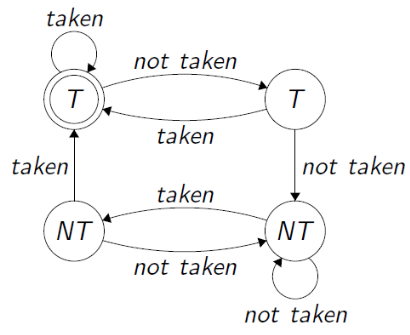
\includegraphics[scale=0.7]{immagini/2bit_pred}\\\\
si possono usare due bit per decidere come spostarsi in base alla predizione. Come si comporta con dei cicli annidati? 
\begin{lstlisting}
	mov $0, %ecx
.outerLoop:
	cmp $10, %ecx
	je .done
	mov $0, %ebx
.innerLoop:
	; actual code
	inc %ebx
	cmp $10, %ebx
	jnz .innerLoop
	
	inc %ecx
	jmp .outerLoop
.done:
\end{lstlisting}
L'unità per la branch prediction continuerà a dire branch taken finché non si arriva a 10, alla fine c'è una decisione sbagliata e si torna al loop esterno. Si cambia continuamente idea per via dell'interazione fra loop interno e loop esterno, per via di questo il 2-bit saturating counter non funziona bene perché sbaglia sempre la prima predizione e l'ultima.\\ La branch prediction è importante, perché da un'analisi risulta che nel codice il 20\% delle istruzioni sono branch condizionali, inoltre ci sono pipeline più complesse e super-scalari, quindi la possibilità di trovare delle istruzioni condizionali è più alta ed inoltre c'è la programmazione ad oggetti, dove per capire se una classe è figlia di un altra bisogna navigare l'albero per capire la classe padre e quindi prendere decisioni.\\ Per migliorare la branch prediction:
\begin{itemize}
\item migliorare la predizione
\item determinare il target prima
\item ridurre la penalità per predizioni errate
\end{itemize}
\subsection{Correlated prediction}
L'idea è che alcuni outcome dei branch sono correlati fra loro, quindi serve poter corralre due branch condizionali in assembly. In un correlated predictor si usa una storia degli m branch passati e si può usare la storia per correlare i branch. Si usa la path history table:
\begin{itemize}
\item si mette la storia globale in un registro globale della storia
\item si usa il valore per accedere ad una pht di 2-bit saturing 
\end{itemize}
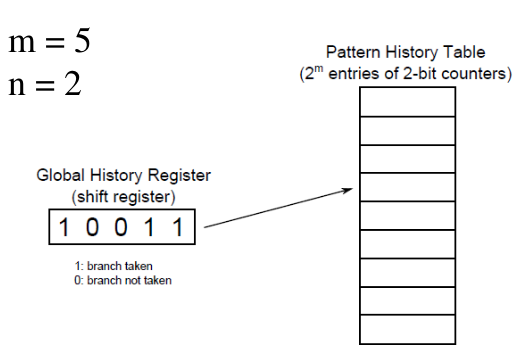
\includegraphics[scale=0.5]{immagini/corr_pred}
\subsection{Tournament predictor}
Si usano due tipi di predittori:
\begin{itemize}
\item correlated predictor, basato sugli ultimi m branches, acceduto dalla storia locale
\item local predictor, che viene selezionato usando l'indirizzo del branch
\end{itemize}
Si usa poi un indicatore di quale è stato il miglior predittore per lo specifico branch in esecuzione, che è un contatore a 2 bit, incrementato per uno dei predittori e decrementato per l'altro. Di seguito, uno schema dell'architettura del tournament predictor DEC Alpha 21264\\\\
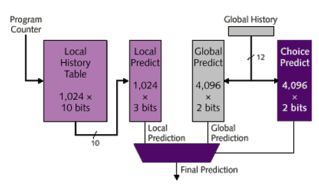
\includegraphics[scale=1]{immagini/tourn_pred}
\subsubsection{Branch target buffer}
È relazionato ai jump indiretti, che sono difficili da predirre. esempio: la ret è l'istruzione di ritorno da una sub routine. Il problema è capire dove si ritorna: qual è l'istruzione che si mette in pipeline, dovrebbe essere la prossima del chiamante ma è ancora più complicato. Si può fare il jump nell'indirizzo contenuto in un registro, l'output dipende da cosa è scritto nel registro che si vuole usare per il salto.\\ Il BTB è una picccola cache che viene acceduta col program counter 
%immagine dell'architettura
troviamo il prefetched target ed il prediction bit, che dice se conviene prendere il trarget oppure mettere uno stallo. È una cache, quindi ci può essere miss o hit, si può imparare se il prefetched target dovrebbe essere quello e più tardi si saprà se quel target è corretto o meno.
\subsubsection{Return address stack}
L'istruzione di ret legge l'indrizzo dallo stack, quindi se possiamo leggerlo subito possiamo sapere il target del ritorno.\\ Possiamo mettere uno stack nella CPU che manitene gli indirizzi di ritorno, ogni volta che c'è una chiamata, si salva in questo stack l'indirizzo di ritorno. In questo modo, ogni volta che si torna si conosce l'indirizzo di ritorno e questo è utilissimo perché l'85\% delle istruzioni è di ritorno.
\subsubsection{Fetch Both Target}
Tecnica che costa molto perché riempi la pipeline con tutte le istruzioni, ma la metà verranno scaratate e non aiuta in casi di fetch multipli come lo \textsf{switch}, non viene usato nell'hardware off the shelf.
%slides
\subsection{Simultaneus multi-threading}
C'è una CPU fisica ma è esposta al software come una coppia di CPU virtuali. L'idea è che mentre runni istruzioni nella pipeline usi un sotto-insieme delle risorse hardware, in questo caso nel simultaneous MT si puà tenere traccia di che hw stanno usando le istruzioni, quindi si duplica lo stato dell'architettura, quindi ad esempio il PC in modo che il processore usi un algoritmo di scheduling in modo da dare il controllo ai differenti thread che girano. Quindi è richiesto meno hw per far girare più processi ma servono dei controlli per evitare l'interferenza.
\subsubsection{Caso Intel: Hyperthreading}
Gli obiettivi sono molteplici:
\begin{itemize}
\item minimizzare la die area
\item evitare che uno dei due processori logici produca stalli per l'altro
\item "spegnere" l'hyperthreading se non necessario
\end{itemize}
Oggi, anche l'archiettura Inter mostra delle istruzioni assembly al programmatore diverse da quelle efeftivamente usate internamente, ci sono due parti:
\begin{itemize}
\item un front-end
\item un engine di esecuzione out-of-order: se puoi eseguire una micro operazione va eseguita immediatamente.
\end{itemize}
\paragraph{Xeon frontend:}il ruolo è quello di tradurre istruzioni CISC in istruzioni RISC usando una microcode ROM. C'è una cache di micro operazioni che mantiene le traduzione già fatte.\\ Nella trace cache, sappiamo se una micro operazione è associata ad uno o all'altro execution program, grazie ai due program counter differenti. Ci sono quindi due code diverse di micro operation. Nel caso di hit: %slides
\\ Nel caso di miss nella TC, serve fare la traduzione: bisogna accedere all'instruction TLB che permette di tradurre la corrispondenza fra indirizzi logici e fisici. Ovviamente, ci sono due TLB associati alla cache L2, quindi si può pagare anche un miss dovuto alla L2. Quindi, si mette la CISC instruction in coda, c'è poi il decoder ROM che mette le istruzioni in una coda usata per fillare la TC e quindi ora si può mettere la micro operation nella $\mu$op queue.
%slides
\paragraph{Xeon Out-of-order pipeline:}
%immagine
vogliamo eseguire le micro operazioni in ogni ordine quando è possibile farlo. Nel primo stadio, vogliamo schedulare i registri fisici della CPU: una $\mu$op cerca di accedere il registro icx, non è uno solo ma sono molteplici, i multi-registri e quindi icx viene mappato su uno di questi. Servono quindi un register rename ed un Allocate per tenere traccia di tutto.\\ Ora ci sono code multiple, per discriminare la semantica della $\mu$op in base al fatto che si acceda alla memoria etc...\\ Lo stadio di execute ha diverse ALU, quindi l'Allocation unit dice anche quale componente usare per eseguire l'istruzione. Lo scheduler prende l'istruzione dalla coda nel momento esatto in cui il componente è disponibile. L'ordine è qualsiasi, le $\mu$op appartengono a diversi program flow, quindi data una CISC operation, le macro istruzioni saranno invertite nell'ordine. \\ Alla fine, non vogliamo che le istruzioni siano materializzate all'esterno in ordine casuale, quindi c'è un reorder buffer per riordinare le istruzioni CISC nell'ordine in cui sono entrare e far credere all'utente siano state processate così.\\ Non abbiamo quindi una idea di come siano state eseguite le istruzioni internamente, quindi ci può essere uno stato di inconsitenza per un tempo illimitato ma non è un problema perché questo non viene esposto a livello ISA. Il problema è che stiamo interagendo con la memoria e questo è sfruttabile, possiamo ad esempio far si che la CPU carichi delle istruzioni che non doverebbe e quindi dei dati in cache che non dovrebbe: l'istruzione non verrà committata, ma la traccia sarà comunque esposta e sfruttabile.
\subsection{Multicores (2000s)}
I vendor cominiano ad usare i molteplici tansistor per creare delle CPU multicore, il primo CPU è l'IBM power4, 2 core con una architettura interessante: una cache privata per ciascun core, interconnessione di un certo tipo fra i core e una cache di L2 ed L3, dove la L3 fa anche da memory controller. I core interagiscono con la L1 e così a salire, quindi per caricare dati dalla memoria. Ma sei i cores hanno una cache privata, come fanno ad essere sincronizzati con i dati contenuti in L1 e quindi visibili al core 2? Serve un protocollo apposito per garantire la consistenza dei dati.
\subsubsection{Cache coherence}
Comportamento della cache da un punto di vista di utilizzo. La CC definisce la coerenza della cache con dei protocolli: quando scrivo codice, non mi rendo conto di interagire con la cache, ma i processori vi interagiscono di conitnuo. Abbiamo ad esempio 2 cores, con due cache private ed una serie di operazioni:
%carica la tabellina
al tempo 0, la cache del core 1 c'è la copia di A, a t=1 C2 carica A in un altro registro. Poi C1 fa una una operazione su A, quindi il valore di A nella cache di C2 quale sarà? Non c'è una sola risposta, dipenderà dal protocollo di consistenza
\paragraph{Strong CC protol:}il protocollo più semplice, tutte le cache dei vedono gli stessi dati, come se non ci fosse una separazione fra le cache in un qualunque istante di tempo. Quindi, serve avere un agreement fra i cores su chi fa l'operazione sul dato, quindi c'è un impatto sulla concorrenza e le perfomance.\\ Per assicurare tale consitenza serve:
\begin{itemize}
\item single write/multiple readers: ad ogni istante di tempo, per ogni locazione di memoria un solo core può leggere e scrivere
\item (slides)
\end{itemize}
Bisogna continuamente sincronizzare le cache quando un core fa un update in memoria, quindi non è molto performante
\paragraph{Coerenza debole:} c'è meno limitazione sulle cache, in quanto devono sincronizzarsi meno, quindi viene persa una delle invarianti dette sopra. Quindi due cores possono scrivere su una stessa area di memoria, quindi può accadere che il programmatore osservi dei comportamenti inattesi e quindi per implementare correttamente l'algoritmo occorre implementare delle primitive software per avere lo stesso outcome che si avrebbe se tutto accadesse sequenzialmente.\\ C'è una time window di un certo numero di epoche temporali in cui i dati non vengono propagati e questo può mostrare la complessità dell'hardware al programmatore\\\\ È anche possibile non avere coerenza, che è il modo per avere le cache più veloci. Non ci sono ovviamente garanzie, quindi le cache vanno sincronizzate esplicitamente lato software, ad esempio con delle API C/Assembly.
\subsubsection{CC protocol}
Un protocollo di consitenza per la cache è un algoritmo distribuito basato su primitive di tipo message-passing. Ci sono due principali tipi di richieste in memoria da servire:
\begin{itemize}
\item Load(A)
\item Store(A)
\end{itemize}
e coinvolge 2 tipi di attori principali, ovvero i cache controllers ed i memory controllers. Il ruolo è quello di rinforzare una certa nozione di coerenza.\\ Qualunque cosa nei protocolli CC è basato sulle coherency transaction, ciascuna di queste genere dei messaggi. Ci sono due tipi principali di transazioni:
\begin{itemize}
\item Get: carica un blocco di cache (dato) in una linea di cache
\item Put: evince un blocco dalla linea di cache, la linea diventa disponbile per altri dati
\end{itemize}
%immagine dell'organizzazione
Ogni linea di cache è associata con un bit che dice se la linea è valida o memo, in questo caso abbiamo una macchina a stati finiti che definisce lo stato del blocco in cache. La macchina è leggermente più complessa di una classi FSM, perché per transitare dai vari stati ci possono essere dei delay dovuti al fatto che il protocollo è distribuito. Ci sono quindi
\begin{itemize}
\item eventi remoti: viene ricevuto un messaggio di coerenza
\item eventi locali, ricevuti dalla parent cache
\end{itemize}
(altro sulle slides)\\ Ci sono una serie di protocolli per gestire la coerenza, definiamo
\begin{itemize}
\item invalidate protocols: protocolli, quando viene scritto un blocco invalida tutte le altre copie.
\item update protocols: ogni update viene mandato a tutti i core.
\end{itemize}
Quindi, nell'esempio iniziale il valore di A dipende dal protocollo implementato. Ci sono poi due famiglie di CC protcolos diversi
\begin{itemize}
\item snooping protocols: tutti i controller osservano tutto il traffico, quindi il broadcast è totalmente ordinato. È molto veloce, perché tutti i controller possono fare decisioni da soli perché osservano tutti i messaggi ma non è scalabile se il numero di core aumenta. Questo perché serve una arbitro del bus, e questo degrada le performance
%immagine snooping
\item directory based: c'è una directory, ogni request è unicast alla directory. Questa tiene traccia di chi è il controller destinatario e gli manda il messaggio, il che rende tutto più scalabile e permette di aumentare il numero di cores.
%immagine directory based
\end{itemize}
\subsubsection{VI protocol}
Il protocollo di consitenza più semplice, un solo cache controller può leggere e/o scrivere il blocco in ogni timestamp.\\ La transaction Get è usata per richiedere un blocco in read-mode per poter diventarne l'owner e potervi scrivere e leggere. La Put è usata per togliere il blocco dalla cache e riscriverlo al LLC controller. Ci sono una serie di eventi:
%copia slides
Il protocollo VI sta per Valid/Invalid, ma oltre a questi due stati ce n'è anche uno intermedio per cui si aspetta una copia del dato up-to-date
%immagine del FSM
Se confrontata con la FSM del LLC, vediamo che c'è differenza: ad un certo punto, il core associato al cache controller fa una operazione di load, quindi ottiene l'indirizzo e va nella cache e scopre che lo stato della cache è I. Quindi, serve una Own-Get dal LCC, manda un messaggio che viene ricevuto da tutti i cache controller nel sistema con un ordinamento totale. Una volta che il messaggio viene mandato, il controller trainsita nello stato IV, la copia verrà inviata dal possessore attuale del dato, dopo averlo ricevuto transita in V. \\ Dopo, un altro core vorrà diventare l'owner e quindi questo controller transiterà nello stato I e trasferirà il contenuto del blocco.\\ Immaginiamo di essere in una situazione in cui c'è un conflitto, ovvero si vuole scrivere un blocco nella linea di cache che è piena. Si manda una Any Put al LLC controller, l'LLC transita nello stato I e se poi qualcuno richiede il dato transita nello stato V.\\ Il protocollo ha una nozione implicita di diryness: se una linea di cache è in stato V, il controller L1 può o leggere e scrivere o solo leggere. Ha anche un concetto implicito di esclusività, in quanto se lo stato è V, nessun altro può accedere al blocco, quindi nessuno ha una copia valida; inoltre, c'è nozione del possesso del blocco: l'owner sarà quello che manda la copia aggiornata a tutti.\\ La cosa positiva del portocollo è che richiede pochi bits per rappresentare le FSM, ma ha diverse inefficienze; ciò che vogliamo catturare del blocco di cache sono aspetti di
\begin{itemize}
\item validità
\item dirtyness
\item exclusivity
\item ownership
\end{itemize}
vogliamo solo queste proprietà per avere un protocollo efficiente ma che consumi più bits per l'implementazione
\subsubsection{MOEST stable states}
Ogni lettera fa riferimento ad uno stato particolare, ognuno cattura una delle proprità dette sopra. Di nuovo, è una FSM per ogni blocco
\begin{itemize}
\item Modified: il blocco è valido, esclusivo, posseduto e potenzialmente dirty.Può essere scritto o letto
\item Owned: blocco valido, posseduto 
\item Shared: valido, non esclusivo, non posseduto, non sporco. Ci sono più copie read only del blocco.
\end{itemize}
(slides)\\ Quali sono le transazioni per poter implementare il protocollo:
\begin{itemize}
\item GetS: Get del blocco in Shared state
\item GetM: Get in modo Modified
\item Upgr: ho un blocco, so che il blocco ha la copia più aggiornata perché ho osservato le transazioni, quindi non voglio la copia del dato ma voglio la possibilità di scrivervi
\item Put (slides)
\end{itemize}
Questa è la macchina a stati che si ha tipicamente: 
%immagine della macchina
\subsubsection{MEST protocol}
Il controller della cache di livello inferiore (LLC) è simile 
%immagine
M/E è uno stato congiunto di Modified/Exclusive. Se in M/E e si osserva una Any-Get, si va in Shared, se qualcuno richiede il blocco, si va in I.
\subsection{Memory Control}
Nelle cache write through, si propaga direttamente l'update.\\ In modern architectures, the cache are no longer write through, due to the complexity can explode.\\ The caches in modern architectures can be either inclusives or exclusives at different levels, this can be exploited by attacks that specifically targets a L* cache.\\ CC dicatates how the different cache controllers interacts among them. There is the concept of memory consistence: il MC model definsce il comportamentio di una memoria condivisa, indipendentemente da come è implementata. Vediamo ancora un esempio:
%tabella esempio
in macchine Multi Core c'è il riordino degli accessi in memoria: il core committa le operazioni sulla memoria in un certo ordine ma gli altri cores possono osservarle in ordine diverso, quindi non c'è un ordinamento totale. Il sotto-sistema può quindi riordinare le operazioni: 
%tabella di esempio
ci sono 4 combinazioni di possibili riordini, quindi se scriviamo codice concorrente, dobbiamo considerare il fatto che ci siano riordini delle operazioni.\\ Questo ha a che fare con due ordinamenti diversi:
\begin{itemize}
\item ordiamento di programma, è per core ed è totale. Cattura l'ordine in cui ogni core 
\item ordinamento di memoria (slides)
\end{itemize}
Possiamo avere diverse consistenze:
\begin{itemize}
\item sequenziale: ci sono determiante operazioni che verranno osservate identicamente tra ordine di programma ed ordine di memoria.\\ Nell'esempio di prima, solo due ordini sono consitenti sequenzialmente
\item consitenza debole: modello implementato dalle architetture moderne. Quella di Intel è Total Order Store. C'è un piccolo buffer che agisce come coda in cui vengono salvate le diverse operazioni di store e che verranno poi processate. Le architetture Intel sono fra quelle in cui c'è il minimo numero di riordini tra le operazioni
\end{itemize}
\subsubsection{Memory fence}
Se ho una qualunque operazioni di memoria, la fence forza l'ordine di una load/store, quindi possiamo creare dei punti in cui siamo sicuri che tutte le istruzioni prima della fence sarà ordinata e stessa cosa se accade prima, ma non si possono riordinare le fence. Sono quindi operazioni speciali che permettono di mettere dei punti di riordino per poter ad esempio avere consistenza sequenziale in Intel.
\paragraph{Fence su architetture x86:} ci sono 3 tipi di fence diverse su x86:
\begin{itemize}
\item MFENCE: barriera full memory, ogni operazione prima e dopo non sarà riordinata
\item SFENCE: barriera store/store
\item LFENCE: barriere load/load e Load/Store
\end{itemize}
\section{In memory transaction}
Le transazioni in memory permettono di realizzare la sincronizzazione in memoria più semplice. Può essere esplicita, quindi per accedere ad un sezione critica si prende un lock, si accede e poi si esce.\\ Ci possono essere problemi sui locks come deadlock, i deadlocks non sono componibili e quindi possono esserci delle inconsistenze nei risultati di operazioni che usano i lock.\\ L'hardware transactional Memory prevede di usare delle istruzioni di Assembly specifiche per dire che su vuole accedere a dei dati in maniera esclusiva, così che il processore metta un lock privato sui dati e una volta finito, se il commit va a buon fine i dati vengano pubblicati all'esterno\\ Per poter implementare le hw transaction Intel ha modificato il protocollo di CC: i tentativi vengono fatti solo al primo livello della cache e si marcano i blocchi di cache con lock, per poi committare se va tutto bene. Ci sono 4 nuove istruzioni Assembly (slides), esempio in C:
% codice del C ed Assembly
Una transazione può andare in abort per vari motivi (slides)\\ Da un punto di vista di performance il problema è per cosa di fa abort a livello hardware, ma la cosa interessante è che la transazione può essere mandata in abort da qualunque altro CPU core.
Se mettiamo di mettere del codice per fare delle transazioni, rischiamo che dopo se mettiamo del codice su quello scritto per fare i lock possiamo avere una esecuzione per cui in concorrenza le cose non tornato (vedi l'esempio dei depositi/ritiri sulle slides), perché i lock non si compongono.\\ Si possono usare le transazioni, concetto preso dal DBMS: quindi, vogliamo eseguire tutte le operazioni fra l'inizio e la fine di una transazione come all or nothing, È possibile farlo sia usando un DBMS, sia tramite l'uso di facilities offerte dall'hardware.\\ La facility hardware è quella delle \textbf{Hardware Transaction Memory}: l'idea dietro è che se nulla va storto, si hanno delle performance migliori. Usati molto negli engine per videogiochi, quasi tutti i processori off the shelf offrono transactional memory, Intel li ha disabilitati quasi del tutto per via di una implementazione buggy.\\ Il paradigma HDM lavora in questo modo:
\begin{itemize}
\item introdurre operazioni Assembly per capire quando inizia e finisce la transazione
\item utilizzo delle cache, i controller sono già in grado di capire se operazioni concorrenti stanno accedendo allo stesso dato e quindi se scoprono un conflitto sui dati, droppano il flusso di esecuzione ed anche i side effects sui dati. Ci sarà poi un retry path
\end{itemize}
Il tipico hardware off the shelf è mostrato di seguito, usato per fare il reverse engineering di come è fatto l'HTM
%immagine dalle slides
la L1 e la L3 possono essere usate per implementare le transazioni, in quanto possono essere usate per rappresentare le transazioni. Ci sono due gruppi di dati, read set e write set. L'implementazione delle HTM introduce un bit aggiuntivo per ogni cache line, che dice se un blocco è stato caricato o letto durante una transazione.\\ Il protocollo di CC sa quali linee sono marcate come transaction access, se se ci sono concorrenze e può agire per rendere lo stato coerente. (slides)
\subsection{Funzionamento}
Le istruzioni assembly usare per supportare HTM sono
\begin{itemize}
\item \textsf{xbegin}
\item \textsf{xend}
\item \textsf{xabort}
\item \textsf{xtest}
\end{itemize}
(vedi slides per dettagli). La cosa buona di questa implemetazione è che sulla base di queste 4 operazioni è possibile scrivere delle transazioni annidate, il che rende la scrittura del codice molto più semplice; il CC controller tiene un contatore delle nested transaction fatte, quando il valore va a 0 pulirà i bit dalla cache.\\ Tutti i compilatori moderni possono generare queste 4 transazioni, a partire da linguaggi di alto livello come C e C++, generando delle Undefined Instruction se HTM è implementato in hardware.\\ Per usare le operazioni, si può scrivere del codice C:
%codice dalle slides.
È possibile capire anche se c'è un abort in corso, quindi è utile se abbiamo una transazione grossa capire se c'è un abort perché magari il processore non è in grado di portarla a commit.\\ Il write set è vicino alla CPU, sta nella L1, mentre il read set è sia in L2 che in L3. Quindi, il cache controller setta il T flag sia in L1 che in L3 quando si legge, mentre solo in L1 quando si scrive. Supponiamo di avere l'esempio del bank account: se ci sono due diversi cache controllers che stanno gestendo le transazioni, non possono conoscere lo stato l'uno dell'altro ma possono verificare che ci sia un accesso concorrente e quindi se ogni altra CPU legge una location di un write set, la transazione andrà in abort: c'è un pezzo dati che è marcato con T, non è ancora committata ed il controller deve mandare il dato più fresco e se c'è una read non può mandare il dato fresco e quindi la transazione deve abortire.\\ Vale lo stesso per le altre CPU: se qualcuno scrive in un read o write set, la transazione va in abort, l'algoritmo è quindi locale al controller, può dare delle performance peggiori per via che si mandano in abort anche cose che non dovrebbero. \\Inoltre ci sono anche limitazioni hw, cosa accade se abbiamo un contex switch: non possiamo lasciare dei dati incommittati nella cache, quindi la transazione deve abortire e lo stesso vale per la ricezione di un interrupt, perché non si sa per quanto tempo si starà in questo stato e non si possono lasciare i dati inconsistenti; lo stesso vale per page faults.\\ Quindi è necessario avere della logica di codice per gestire gli abort\\ I codici di errore possono essere vari
\textbf{esempio:}\\ abbiamo una transazione, vediamo l'effetto sulla cache
%codice dell'esempio
Abbiamo solo due locazioni di memoria coinvolte nella transazione, vediamo cosa accade in una possibile run concorrente:
\begin{itemize}
\item $CPU_0$ legge $a_0$ dalla cache e setta il T bit
\item $CPU_0$ scrive su $a_0$, portando quindi lo stato a modified, quindi $a_0$ è nel write set
\item $CPU_1$ legge $a_1$ nella cache (in maniera esclusiva) e setta il T bit
\end{itemize}
Lo stato della cache è il seguente:
%slides
quindi è possibile committare semplicemente pulendo lo stato dei bit.\\ Se $CPU_1$ entra in gioco e legge $a_0$, la $CPU_0$ deve per forza fare abort: pulisce i T bit e rende le linee di cache invalide che erano Modified. Ora, $CPU_1$ deve per forza leggere i dati dalla memoria, perché in cache sono invalide, questo avviene proprio quando $CPU_0$ stava per fare il commit.
\section{Recap sulla gestione della memoria virtuale}
La memoria virtuale serve per far si che le applicazioni non accedano alla memoria fisica direttamente, bensì tramite degli indirizzi virtuali. L'idea è do astrarre cosa una applicazione vede e cosa il processore dovrebbe fare, per molteplici motivi
\begin{itemize}
\item rendere la scrittura del codice più facile;
\item ingannare l'applicazione, facendole credere di avere più memoria in quanto si può fare lo swapping sulla memoria;
\item isolamento per processo: se qualcuno nel sistema può trasformare un indirizzo virtuale in uno fisico ed il componente è abbastanza sicuro, ci sono delle delimitazioni che impediscono ai processi di vedere i dati di altri processi, a meno di usare memoria condivisa
\end{itemize}
Il supporto alla memoria virtuale usa sia hardware che firmware, che OS (slides).\\ Usiamo la terminologia di virtual page e di segmento di memoria: una pagina virtuale viene mappata su un un frame fisico.
%immagini
è possibile che un certo range degli indirizzi virtuali condividano dei frame fisici in memoria. IL firmware deve fare diverse operazioni per poter usare le pagine virtuali, quindi viene introdotto una cache addizionale per facilitare la traduzione tra virtual e phisical address: TLB, che se ha la traduzione in memoria da l'indirizzo fisico corrispondente all'indirizzo virtuale.\\ I passi della traduzione sono riassunti di seguito:
%immagine slide
si può avere un indirizzo virtuale valido, che però non è presente nella memoria fisica per via dello swapping, quindi si ha un miss nel TLB o nella page table.
\subsection{Traduzione in x86}
Le CPU Intel sono bloated, quindi cercano di fare di tutto per dare retro-compatibilità, quindi ogni volta che c'è una nuova facility viene disabilitata per default, quando parte un nuovo chip Intel è come se fosse un 8086, ci pensa il SO ad abilitare tutto ciò che serve:
\begin{itemize}
\item segmentazione di memoria
\item segmentazione di memoria in protected mode
\item paginazione
\end{itemize}
L'indirizzamento basata sulla segmentazione è fatta in base a questo schema:
%immagine dalle slides
Come funziona l'unità di segmentazione: 4 registri a 16 bit (allo startup girano così) per i segmenti
\begin{itemize}
\item CS: code segment, dove trovare il codice in memoria
\item DS: data segment, dove trovare i dati in memoria
\item SS: stack segment
\item ES: extra segment
\end{itemize}
Intel i386 ha aggiunto due nuovi registri, FS e GS senza uso predefinito.\\ Basandosi sulla segmentazione, si possono definire dei segmenti di memoria in cui ogni segmento è un numero che indica l'inizio del segmento, quindi è possibile avere overlapping. Un esempio è mostrato in seguito:
%immagine delle istruzioni Assembly dalle slides
\subsubsection{Registri x86\_64}
%immagine dei registri
fra i tanti registi, i due di interesse sono (slides). Abbiamo bisogno di strutture dati, che è un virtual-to-phisical tree che mantiene le tabelle di traduzione e la cui root è indicizzata da CR3.
\subsubsection{Segmentazione protected mode}
%immagine
tra le informazioni che otteniamo, dovremmo avere la base dell'indirizzo ma in realtà si ha un indice che serve per accedere ad un tabella in memoria centrale. La tabella ha dei segment descriptor che mantengono i base address per i segmenti,può essere ovunque in memoria per cui si può avere l'indirizzo nel registro GDTR. Supponiamo di avere una jmp che ha un target: l'indirizzo diventa un offset, nel CS register si trova un indice nella global descriptor table. A quel punto si usa l'index come offset nella tabella e trova il segment descriptror, quindi si prende la base e si somma all'offset per ottenere un indirizzo logico.\\ La base è sempre 0, per via della retro-compatibilità, ma il processo va comunque fatto per rendere possibile la paginazione (lo fa il SO). Quando rendiamo possibile la paginazione, l'indirizzo è lineare e viene passato all'unità di paginazione (firmware) che lo trasforma in un indirizzo fisico e lo passa alla CPU
\subsubsection{Unità di paginazione}
L'idea è che l'indirizzo lineare viene diviso in 3 pezzi (32 bit):
\begin{itemize}
\item directory: indice alla tabella puntata da CR3
\item Table: indice nella page table
\item offset, che viene usato per trovare l'indirizzo fisico del frame
\end{itemize}
%immagine
ogni tabella ha nel record un puntatore al componente successivo, sono tutte mantenute in memoria e la gestione è fatta dal SO. C'è un albero di tabelle per ogni processo. Quando si fa context switch, il valore del CR3 non viene cambiato e quindi è possibile anche trovare indirizzi del kernel.
\subsection{Traduzione Virtual-to-phisical i386}
L'istruzione assembly ha un indirizzo logico, che verrà usato come offset per la tabella dall'unità di segmentazione per ottenere un indirizzo logico, che verrà usato dalla page table per navigare una pagina ed ottenere un indirizzo fisico da passare alla CPU. Ogni volta che si accede ad un singolo byte di memoria si triggera tutto il processo
%immagine
quindi per questo è stato introdotto il caching, per cercare di ridurre la latenza. Per usare l'indirizzo fisico, il cache controller deve aspettare che tutta la traduzione avvenga, se si usa solo l'indirizzo logico c'è un problema se le tabelle cambiano.\\ È possibile usare entrambe le cose: appena l'applicazione genera un indirizzo lineare, questo viene preso dal firmware del cache controller L1, e se il dato è in memoria c'è un hit. In parallelo c'è il controllo nel TLB per vedere se è possibile tradurre in indirizzo fisico. Se c'è un miss nel TLB parte la traduzione per ottenere l'indirizzo. Quindi diversi livelli di cache sono indicizzati con diversi indirizzi, per cercare di velocizzare il processo di traduzione si fanno diverse cose in parallelo.
%immagine riassuntiva
\section{Primitive di lettura}
Vogliamo trovare un modo per bypassare l'isolamento dei processi, la tecnica da usare sarà il timing: vogliamo mettere su delle primitive di lettura, l'idea fondamentale dietro la sicurezza è che non vogliamo lasciare delle informazioni, a volte anche il tempo impiegato per fare un'operazione dice qualcosa. 
\subsection{Algorithm Timing}
Prendiamo il seguente esempio:
\begin{lstlisting}
int strcmp(char *t, char *s){
	for( ; *t == *s ; s++, t++){
		if(*t == '\0')
			return 0;	
	}
	return *t - *s;
}
\end{lstlisting}
passando le due stringhe "ABCD" ed "ABxDE" possiamo inferire qualcosa dai dati in base al tempo impiegato per fare il confronto.\\ Useremo degli approcci simili sulla cache: ogni volta che leggiamo i dati dalla CPU, questi vengono letti dalla cache e quindi ogni volta che si fa una load, a seconda della della condizione, ci saranno differenti risultati
\begin{itemize}
\item supponiamo di avere la cache in modified, siamo i proprietari e possiamo leggere
\item se il blocco è invalid, occorre fare altre azioni
\end{itemize}
dipende tutto dallo stato in cui è la FSM della cache. L'idea è che possiamo fare delle operazioni sulla cache privata in modo da portare la FSM in degli stati che conosciamo, quindi per fare un side channel
\begin{itemize}
\item portiamo la cache in uno stato noto
\item facciamo si che qualcuno faccia delle operazioni sulla cache per cambiarne lo stato
\item vediamo, tramite timing, come è cambiato lo stato
\end{itemize}
con l'hyperthreading è ancora più critico, perché ci sono più thread che girano sullo stesso core e quindi condividono la stessa cache L1 e quindi potremmo leggere i dati di qualcun altro e quindi violare la privatezza della L1 per via del simultaneous MT; ((NB: se non ci fosse, la L1 rimarrebbe privata. Inoltre, la L1 di usa indirizzi virtuali per indicizzare i blocchi dati, quindi è anche più semplice accedere ai dati.))
\subsection{Code path}
Ci sono degli algoritmi su cui non si può fare timing, perché l'algoritmo ci metterà sempre lo stesso tempo. Ad esempio abbiamo il Montgomery Ladder, usato per fare operazioni sulle curve ellittiche e blocco chiave della crittografia. Abbiamo delle nonce, che devono essere univoche altrimenti si potrebbe invertire la curva (ricavare la chiave privata), lo pseudocode è il seguente:
%codice dell'algoritmo
abbiamo k bit, ma il numero di operazioni è sempre lo stesso. Accediamo allo scalar, 1 bit alla volta, ed a seconda del valore accediamo ad uno dei rami dell'if-else e quindi ci chiediamo se possiamo determinare in quale dei due branch siamo, sfruttando la L1 per ricavare la nonce. Una volta che il codice è caricato, viene messo in cache ed alcune operazioni sono grandi e quindi finiscono su più linee di cache, quindi se riusciamo a portare lo stato della gerarchia della cache in modo da capire in quali linee di cache è stato eseguita l'operazione, possiamo sapere se è stato preso l'if o l'else.\\ Quindi, anche se l'algoritmo è time independent, possiamo osservare quali linee di cache sono state usate per accedere ai dati
\subsection{Side channel attacks}
Un side channel è una zona di memoria che permette di leggere un altro contenuto di memoria o accedere a dei pattern di dati. Ci sono diverse tipologie di side channels
\begin{itemize}
\item Prime + Probe
\item Flush and Reload
\item Flush + Flush
\item Evict + Time
(slides)
\end{itemize}
l'idea è sempre che la prima parte viene usata per portare la cache in un certo stato, con la seconda si cerca di capire dopo che la vittima ha fatto qualcosa, qual è il side effect sullo stato della cache. Non c'è nulla che il SO può fare per garantire l'isolamento dei processi, perché lo stato dell'hardware è condiviso. Un attacco passa per diversi stati, le differenti macchine cambiano per diversi aspetti quindi abbiamo
\begin{enumerate}
\item pre-attack: il pre-target attack serve per acquisire il target, quindi ad esempio la linea di cache o il cache set (nel caso di cache n-associative ) stabilire eventuali timing threshold. Dobbiamo considerare tanti elementi, come ad esempio il carico di lavoro della macchina, se è alto potremmo essere deschedulati e perdere ad esempio la CPU su cui stavamo lavorando venendo rischedulati su un'altra
\item active attack:
\begin{itemize}
\item[a)] Inizializzazione: portare il canale in uno stato noto
\item[b)] Attendere che la vittima faccia un accesso in memoria
\item[c)] Analizzare l'accesso, osservando i side effects lasciati dalla vittima
\item[d)] Ripetere l'accesso fino al leak dei dati
\end{itemize}
\end{enumerate}
Ci sono diversi aspetti da considerare
\begin{itemize}
\item Le cache sono cachate sia virtualmente che fisicamente
\item le cache sono condivise in maniera differente in base al livello
\item vanno considerati anche gli interleave di esecuzione fra i diversi processi
\end{itemize}
mettere su un vero side channel attack è molto più complesso di cosa si legge nei paper
\subsubsection{Evict + Time}
Il target è la cancellazione di una linea, quindi inizialmente la vittima gira e fa degli accessi in memoria, quindi carica i suoi dati in memoria. A questo punto, stabiliamo una baseline execution, ovvero sappiamo che la vittima girerà di nuovo e quanto ci metterà quando ha i dati in cache. L'attacker quindi cancella una linea di interesse dalla cache per scoprire se la vittima la usa: in algoritmi crittografici, si ci basa su tabelle di dati condivise che vengono usati in base alla chiave. Quindi se sappiamo quale parte della tabella viene usata, possiamo fare una ricostruzione di discovery code path, quindi capire quale parte dell'algoritmo viene usato mentre gira. Questo stato effettivamente usato per rompere AES, possiamo scoprire quali linee di cache sono state usate per capire ad esempio la chiave di cifratura, usando il tempo: vediamo quanto ci vuole per fare degli accessi per capire se la vittima sta usando una cache line cancellata o no.\\ La parte critica è poter far girare la vittima quando si vuole, ad esempio è stato usato per rompere AES perché è una libreria condivisa e quindi è possibile per l'attaccante far girare la vittima.\\ Non usare solo l'istruzione Assembly \textsf{rdtsc} per contare il tempo che passa, i chip del processore vengono spenti/accesi in base alla temperatura del processore (perché si tocca il power wall) così come anche viene \textbf{decrementata la frequenza del processore}, quindi il numero di cicli effettivi contati è falsato. Usiamo l'istruzione \textsf{rdtscp} perché rispetta il program order, altrimenti bisognerebbe usare le fence (ricorda l'esempio di Quaglia). La cosa interessante è che l'attacco è veloce quanto la vittima è veloce nel computare.\\ Nota: nel codice, vengono usati buffer di caratteri di 4096 byte, perché? La gerarchia delle cache sono state introdotte nel calcolatore per sfruttare la località in modo da fare andare tutto più velocemente. Uno dei principi è la \textbf{località spaziale}, quindi possibilmente se viene caricata una linea di cache, anche se viene caricata una sola linea e quella successiva è associata ad uno stato invalid, la cache potrebbe pre-fetchare una linea di cache. Quindi, dobbiamo considerare il pre-fetching quando buildiamo un attacco, essendo sicuri che le linee pre-fetched vengano flushate. 4KB è una pagina ed è talmente grande che anche col pre-fetching siamo abbastanza sicuri che non ci siano effetti indesiderati dopo la flush della linea di cache.
\subsubsection{Flush + Reload}
Basato sull'abilità di usare memoria virtuale condivisa, quindi affinché funzioni il pre-requisito è che sia possibile condividere i dati virtualmente con un altro processo, quindi diverse applicazioni condividono pagine di memoria per risparmiare spazio (si usa la copy on write, appena si cambia un byte si duplica la pagina). Flushamo una linea di cache, possiamo farlo con un indirizzo virtuale, eseguiamo la vittima e poi proviamo a ricaricare le linee di cache flushate prima e misurare il tempo. Se flushamo la linea e viene ricaricata dopo un po', nessuno l'ha toccata, altrimenti vuol dire che una vittima ha toccato quella linea di cache e quindi una parte di dati. La vittima viene fatta girare una volta sola, se non c'è noise sulla gerarchia di cache basta girare una volta sola.\\ Nel codice, viene allineata la pagina di cache, la prima cosa che si fa è materializzare il vettore di probe in memoria: l'approccio di Linux è che il kernel non si fida dello sviluppatore, quindi se chiede molta memoria l'OS ne da di meno se si accorge che è fatto di zeri. Quindi, l'indirizzo di memoria virtuale è valido, ma non è mappato in memoria fisica del tutto, c'è una pagina in Linux che è piena di 0 (la zero page) che viene condivisa da tutte quelle strutture con tutti zeri. In questo modo si dice al kernel che si vogliono davvero le 256 pagine, semplicemente scrivendo un byte.\\ Ora, bisogna discriminare fra cache hit e miss e mettiamo delle lfence per essere sicuri che non ci sia della noise aggiuntiva per via della memory consistency.\\ NB: nell'attacco, creiamo una pagina per ogni singolo valore del byte che andiamo a leggere. Quindi nell'accesso in \textsf{make\_side\_effect} leggo una pagina della memoria prendendo uno qualsiasi dei valori del byte, quindi creo un pointer in una delle pagine del vettore che verrà portata in cache, che sarà associata al valore del byte. Se troviamo la pagina numero 0 in cache, vuol dire che il valore del byte è 0, se invece trovo la pagina 1, vuol dire che il byte letto è 1 e così via.\\ Quindi, mi baso su due cose
\begin{itemize}
\item uso la grandezza di una pagina per mitigare il cache pre-fetching
\item carico un valore in memoria senza far girare la vittima. Se ho l'indirizzo di memoria virtuale e posso leggere un valore in memoria, posso leggere un valore, portarlo in un vettore e poter vedere se quel byte viene acceduto
\end{itemize}
perché non leggere direttamente il valore del puntatore? L'indirizzo può essere valido, ma non è detto che siamo in grado di leggere perché non abbiamo privilegi di lettura in memoria.\\ Otteniamo un seg fault se la memoria non è valida, ma lo possiamo gestire con un handler e continuare con l'esecuzione e quindi possiamo bypassare i privilegi di accesso perché abbiamo portato dei dati in memoria. Questo è il fondamento di meltdown.
\subsubsection{Prime + Probe}
Si fa girare in cache L3, non serve per forza SMT, si può anche lavorare fra diverse VM. La tecnica prevede di fare un priming della cache, ovvero portarla in uno stato noto caricando dei dati che conosco in cache, mettendo uno o più linee di cache che riempano tutte le linee in quanto la cache è set-associativa.\\ Una volta fatta girare la vittima, questa deve invalidare delle linee di cache e carica i suoi valori, a questo punto possiamo rigirare e fare il probing del cache set caricato prima tramite una operazione di probing: se il tempo di accesso aumenta, sappiamo che la vittima ha toccato quelle linee di cache.\\ Un attacco di successo di Prime + Probe non è così semplice perché mettere su un cache set non è così semplice in una cache set-associativa
%immagine
Ci sono delle contromisure hardware, il mapping memory-to-cache cambia di continuo (slides)\\ L'unico modo per mettere su l'attacco è conoscere il mapping a run time:
\begin{itemize}
\item scegliere N indirizzi di memoria casuali. C'è la possibilità di un cache collision perché non conosciamo il mapping con la memoria
\item misuriamo il tempo che ci vuole per caricare la cache accedendo agli indirizzi di memoria
\item se becchiamo una self cache collision, rimuoviamo l'indirizzo dal set. Possiamo usare CPUID per capire l'architettura della cache
\end{itemize}
\subsubsection{Prime + Abort}
Permette di fare tutto ciò che è stato detto fin ora senza timing. Tramite le transactional memory, avremo delle hardware callback che ci dicono che c'è stato un accesso in memoria. L'idea è quella di fare una transazione, aspettare per un abort e nel momento in cui l'abort avviene sappiamo chi ha fatto l'accesso alla memoria (slides).\\ Possiamo anche mettere su degli attacchi alla cache L3: una linea di cache scritta durante una transazione viene tolta dalla L1, quindi l'accesso transazionale fa una write in memoria (slides)
\subsubsection{Flush + Flush}
La clfush non è idempotente rispetto al timing, quindi a seconda dell'input ci metterà tempo diverso. Facciamo una clflush e la CPU dice al cache controller di fare un flush ma a seconda dello stato della cache il tempo impiegato sarà diverso. È una versione del Flush + Reload che permette di capire se la cache line è stata invalidata da qualcuno. È molto stealthy come attacco, perché non si fa molto rumore ed inoltre è veloce. Quindi, anche la \textbf{bandwidth} dell'attacco è aumentata, perché il numero di dati che si riescono a scoprire è maggiore.
\section{Out of order pipeline}
Usando i side channel attacks visti, vediamo cosa possiamo fare introducendo la out of order exection pipeline: possiamo fare il leak dei dati, se facciamo girare le micro-istruzioni in pipeline in maniera speculativa. L'architettura non è quindi sicura al 100\% se le micro-istruzioni verranno portate a termine, lo fa per velocizzare la pipeline ed alla fine ci può essere il commit o lo squash della pipeline se i check sulla istruzione non torna: se viene fatto il commit, le conseguenze verranno esposte sull'architettura della CPU, altrimenti no. Ma anche se la CPU capisce che una operazione fallisce e non deve essere portata a commit, le conseguenze sulla micro-architettura ci sono: se facciamo una micro-operazione che fa accesso sulla cache, gli effetti rimangono anche se l'istruzione viene tolta dalla pipeline. Questo è l'effetto degli attacchi di tipo \textbf{Transient Execution}, attacchi come
\begin{itemize}
\item Spectre
\item Meltdown
\end{itemize}
che sono usciti nel 2018, ma la comunità di ricerca aveva già intuito della loro potenzialità 10 anni prima. Per riassumere
\begin{itemize}
\item eseguiamo istruzioni speculative nella pipeline
\item possono essere rimosse, ma gli effetti rimangono nello stato micro-architetturale
\end{itemize}
\subsection{Meltdown primer}
Questo è un primo esempio di codice per fare meltdown:
%codice
mettiamo su un probe array, abbiamo una pagina per ognuno dei possibili valori di un byte, quindi facciamo il leak di un byte alla volta. Non vogliamo leggere il byte, ma misurare l'effetto delle esecuzioni transienti, per capire se alcuni dati sono stati acceduti durante una esecuzione speculativa.\\ Facciamo il flush del contenuto dell'array dalla cache. Ora, cerchiamo di accedere degli indirizzi di memoria, ad esempio di un buffer del SO e cerchiamo di de-referenziarlo, quindi di leggere un byte.\\ Il kernel non vuole esporre all'utente le strutture dati usate, quindi l'indirizzo del kernel non è leggibile dall'utente e quindi ogni volta che proviamo ad accedere c'è un SEGFAULT:
\begin{itemize}
\item cerchiamo di accedere ad un indirizzo
\item passiamo un indirizzo virtuale
\item viene tradotto in fisico tramite la page table, c'è un bit che dice che non si può accedere
\item il SO manda una trap e viene eseguito del codice per gestirlo
\end{itemize}
siccome il SEGFAULT è un segnale, si può intercettarlo e fare recovery, come ad esempio dire al SO di continuare a girare.\\ L'attacco è utile in quanto la traduzione indirizzo virtuale-fisico ha bisogno di tempo, siccome giriamo speculativamente, l'istruzione viene lasciata in pipeline per un certo intervallo di tempo. L'attacco funziona per un bug della CPU, poiché se possiamo fare la traduzione dell'indirizzo del kernel il firmware sa già che quell'indirizzo non è accessibile a livello user, ma per via di un design errato della CPU questo controllo viene fatto a ret time. Infatti, CPU come ARM ed alcune AMD questo check viene fatto subito e quindi non sono vulnerabili a questo tipo di attacco, cosa che non avviene in Intel CPU: quindi, in questo caso viene comunque fatta la load nella cache, ma l'attacco in se non ha molto senso di esistere.\\ Ora ci sono delle patch hardware per cui non si soffre più di questo problema: l'istruzione viene considerata phantom, quindi non completerà mai, alla fine dell'esecuzione verrà squshata.\\ Quindi per via di un design sbagliato della CPU, il cache controller fa comunque operazioni di load dell'indirizzo per una istruzione che è doomed e quindi non verrà mai committata. Abbiamo quindi un byte, lo moltiplichiamo per la taglia di una pagina, quindi il byte diventa la probe page nel probe array e quindi un offset con cui possiamo accedere all'address space dell'attacker, ma l'accesso dipende da un byte letto speculativamente. Viene quindi caricata una pagina in cache, ora so che ho rimosso tutte le pagine tranne quella appena caricata e posso fare il timing sulla mia stessa cache di quale di queste pagine è stata caricata.
\subsection{Inganno della branch prediciton unit}
L'unità per la predizione dei branch serve per aiutare nella decisione delle istruzioni di salto, quindi dire quale è il migliore valore di guess per una istruzione di salto. Il predittore impara dal passato recente, che però dipende dalla mia applicazione: quindi possiamo fare del poisoning della BPU per fargli fare quello che vogliamo. Eseguiamo una istruzione voluta molteplici volte per fargli capire qual è l'outcome della istruzione, dopo del tempo la BPU diventerà stabile e quindi l'outcome sarà sempre lo stesso. All'improvviso, cambiamo il flusso del codice, quindi verrà fatto un guess errato che era quello che volevamo, ma se il guess è errato il check verrà fatto dopo nella pipeline, intanto verrà fetchata l'istruzione in pipeline e se possiamo controllare le istruzioni, siamo in uno scenario simile al precedente.\\ Qui serve uno step addizionale rispetto a meltdown perché va fatto il trainign della CPU
\subsubsection{Spectre v1}
Facciamo girare del codice un numero elevato di volte
\begin{lstlisting}
if (x < array1_size){
	y = array2[array[1x] * 4096];
}
\end{lstlisting}
il valore di x però viene usato per accedere una pagina in un probe array, come in meltdown. Per far si che funzioni, dobbiamo essere sicuri che \textsf{array1\_size} non sia in cache, perché vogliamo che il cache controller starti una transazione per portare in cache il valore. La BPU farà un guess sull'outcome dell if, in modo che se lo facciamo spesso la BPU dirà sempre branch taken, non avendo il valore in cache aumentiamo il tempo per cui il guess fatto dalla BPU sarà vero o no. \textsf{array1[x]} è il byte di interesse, ma nel momento in cui x non sta nei limiti, saltiamo da qualche parte nell'address space, questa cosa viene fatta dopo un certo tempo.  L'attacco è molto più difficile da patchare: non avendo array1 in cache, non ci sono check che la CPU può fare in anticipo, mentre nel caso di meldown il bit di accesso è sempre disponibile. In questo caso il dato non è in cache, il controllo viene appositamente dilazionato, l'attacco va a cambiare il corretto funzionamento della BPU e del funzionamento interno della CPU.
\subsubsection{Spectre v2}
Variante di spectre, fin ora abbiamo visto attacchi per cui il codice per l'attacco era nel processo dell'attaccante. Possiamo fare una variante in cui il codice non è nell'address space: cerchiamo una porzione di codice in un altro processo, un buon candidato è codice di livello kernel, o librerie condivise, programmi eBPF. Scegliamo un \textbf{gadget} dall'address space della vittima, ovvero un insieme di istruzioni valide generate dal compilatore per essere eseguite in un certo ordine. Quindi, cosa succede se vengono eseguite in un altro ordine, ovvero ad esempio eseguendole all'interno di una funzione, possiamo fare jump ovunque cambiando il valore del PC, quindi anche fuori dalla logica del mio programma.\\ Dobbiamo poter ispezionare il codice dell'applicazione e saltare da qualche parte, quindi al gadget nell'address space della vittima. Di nuovo, facciamo il poison della BPU, possiamo far girare la funzione corretta in modo da avere un certo comportamento, dopo un certo numero di guess cambiamo le pre-condizioni del gadget, quindi saltiamo direttamente al gadget, quindi il vero payload dell'attaccante è il gadget della vittima che è codice legittimo, semplicemente lo usiamo in maniera impropria, ad esempio saltando nel mezzo di una funzione.\\ Esempi:
\begin{lstlisting}
adc edi, dword ptr [ebx + edx + 13BE13BDh]
adc dl, byte ptr[edi]
\end{lstlisting}
istruzioni di Win10, accediamo alla memoria con queste due istruzioni. Le istruzioni sono parte di una funzione più grande, vengono usate per calcolare qualcosa nel kernel, l'unica cosa che mi interessa è che usano quei due registri: se riesco a controllare quei registri e fare il jump a quelle istruzioni, posso controllare i valori. Per controllare le istruzioni, dobbiamo assicurarci che la BPU faccia un guess sul contenuto dei valori. La funzione gira molteplici volte, in modo che la BPU associ alla prima istruzione un certo otucome, la BPU fa il check sul fatto che io possa o meno accedere alla memoria, facendo così la BPU farà semplicemente girare l'istruzione, facendo side effect in cache, e poi la CPU si renderà conto che magari va squashata, ma ormai possiamo misurare i side effects.\\ Per sfruttare le istruzioni, possiamo impostare edi all'indirizzo di base di un certo probe array: vogliamo accedere ad m, quindi dobbiamo sottrarre i valori che vengono sommati nell'istruzione: \textsf{ebx = m - edx - 13BE13BDh}. Quindi stiamo controllando come usare m, la prima istruzione leggerà sempre il mio indirizzo di memoria m, il valore viene aggiunto al registro edi, ma edi sta puntando al mio probe array. La seconda istruzione carica nel probe array il valore m, quindi possiamo far girare qualunque codice del kernel, shared library etc.. in modo da accedere al mio probe array. Il codice è legittimo, accediamo la memoria su una struttura dati controllata da me, il probe array, quindi accediamo a nostro piacimento ed il codice non è semplice da patchare.\\ Ci sono le convenzioni delle chiamate a funzione: se chiamiamo delle chiamate a funzione, il caller deve assicurarsi che i valori siano salvati, se saltiamo nel mezzo di una funzione, il compilatore non si cura del valore perché da per scontato che il chiamante abbiamo salvato lo stato dei registri. Il compilatore genera il codice pensando che questo verrà usato sempre rispettando le convenzioni delle chiamate, ma se si salta nel mezzo della funzione, si può eseguire del codice gadget a nostro piacimento. 
\section{Mitigare i side channels}
In generale, gli attacchi basati su timing sono complicati da patchare perché si usano i meccanismi interni della cache. Quindi, dovremmo poter implementare delle operazioni idem-potenti che non diano leaks sul tempo. Ma cercare di nascondere la differenza fra hit/miss della cache e per poter riuscire a liberarsi di questi problemi occorrerebbe non usare la cache che non ha senso.\\ Si potrebbero applicare una strada più dura, quindi ad esempio restringere dei timer ad alta risoluzione come la rdtsc, ma spesso le operazioni sono necessarie. Si potrebbero marcare determinate regioni di memoria come non raggiungibili, ma è molto challenging dal punto di vista hardware.\\ Abbiamo detto che spesso si sfrutta AES come "vittima" per questi attacchi, qui si potrebbe implementarlo completamente in hardware, ma per gli altri algoritmi di cifratura? O se la CPU non ha questa possibilità?\\ Altra possibilità è implementare gli algoritmi in modo che ai dati segreti non sia permesso di influenzare gli accessi in memoria. Per gli attacchi basati sulle istruzioni transazionali, si può disabilitare TSX oppure buttare la OOO-pipeline, che però è performance-critical.\\ Fin ora questi attacchi sono sulla L1, per patchare gli attacchi a questa cache si può disabilitare il SMT (Sim Multi-threading), quindi in pratica per rendere il sistema sicuro consiste nel disabilitare tutto quello che è stato introdotto per essere più veloci.
\subsection{Detection way}
L'idea dietro la rilevazione dei side channel: il side channel spesso porta la cache in stato noto in una fase di prepare, quindi c'è molto rumore sulla cache, vengono fatte molte operazioni. Le CPU moderne (dai 90) hanno degli HPC (Hardware Performance Counter): perf è uno user space tool che aiuta a capire se ci sono dei bottle-necks nell'applicazione, per farlo il tool usa dei registri counter che sono programmabili dal SO:
\begin{itemize}
\item contare il numero di miss in cache L1
\item contare il numero di flush nella L3
\end{itemize}
i conter sono efficienti perché collegati tramite fili direttamente ai counter hardware. Quindi, se verifichiamo gli effetti più comuni sull'architettura della cache, possiamo creare dei profili di utilizzo dell'architettura di cache per scoprire se sono state fatte determinate operazioni sulla cache. Il problema è che questo tipo di tool sono molto volatili e cambiano spesso, inoltre hanno dei bug perché non sono critici per l'esecuzione delle applicazioni.\\ I problemi per un approccio basato sulla mitigazione: la cache funziona bene perché è basata sul principio di località, se l'applicazione lavora con una mole di dati eccessiva, continuerà a richiedere dati dalla memoria ed a portarli in cache e quindi non possiamo essere al 100\% sicuri che l'applicazione sia malevola, quindi non possiamo usare questo tipo di tecnica ad esempio per far carshare le applicazioni. Potremmo, se c'è SMT attivo, impedire di far girare un altro processo sulla stessa CPU. L'attaccker può aggirare questo tipo di controllo facendo sleep di 1h (ad esempio) dopo il leak di ogni byte, per diminuire il bandwidth dell'attacco, quindi di nuovo non possiamo scoprire l'attaccante con sicurezza.\\ Quindi in generale non è possibile mitigare i side channel attacks.
\subsection{Mitigare le transient execution: kernel isolation}
Solitamente, nella memoria abbiamo la parte alta dedicata al kernel ed un'altra dedicata allo user space. Nella page table, ci sono i bit che dicono se si può o meno accedere all'indirizzo fisico, ma questo controllo viene fatto dopo nella pipeline, quindi per evitare che l'indirizzo sia caricato è andare a rimuovere l'indirizzo dalla page table. L'unico modo a livello software è impedire all'applicazione il mapping fra memoria virtuale e fisica, cos la CPU fermerà subito l'esecuzione perché non ha l'indirizzo della memoria valido. L'unico modo è cambiare come il SO viene mappato in memoria virtuale, ovvero usare la kernel page table isolation, tradizionalmente l'organizzazione era del kernel sopra lo spazio user, oggi cambia se siamo in kernel mode o user mode:
\begin{itemize}
\item in kernel mode le strutture sono le stesse
\item in user mode, la gran parte del kernel space non è mappata: se cerchiamo di fare leaking del byte, non otteniamo nulla perché la memoria non è mappata su memoria fisica e quindi non ci saranno side effects in memoria.
\end{itemize}
Quindi
\begin{itemize}
\item come facciamo ad applicare questo meccanismo, ovvero cambiare la visione velocemente: la traduzione funziona perché CR3 mantiene l'indirizzo della page directory. Il SO riserva una sola entry per il kernel level, se abbiamo due versioni differenti della Page directory, in cui in una la entry del kernel è valida e nell'altro no, possiamo switchare le tabelle a seconda della mode con cui stiamo girando. Per cui, ogni volta che passiamo a kernel mode, nel codice della \textsf{cpu\_entry\_area}, il sistema aggiorna in contenuto del CR3 per cambiare la first level page table usata dal firmware. C'è un componente hardware addizionale, perché fare la traduzione tra indirizzo fisico a virtuale, ma c'è il TLB dove potrei aver cachato le traduzioni degli indirizzi del kernel: quindi ogni volta che si cambia il contenuto del CR3 va flushato il TLB.\\ Questo è un esempio del codice del kernel
%copia codice
ogni volta che si chiama il kernel, si flusha il TLB due volte perché si chiama il CR3 due volte, quindi per questo le performance delle applicazioni droppano tantissimo se si leggono/scrivono parecchi dati su/dal disco usando molte syscall.
\item perché c'è una piccola parte di kernel mappata: ci sono le pagine tradotte da indirizzo virtuale a fisico per lo user space, se c'è un miss nel TLB occorre fare la traduzione. Si deve avere la possibilità di gestire un hardware interrupt, servono le informazioni minime per gestirle ed inoltre serve il codice minimo per entrare in kernel mode, in modo da fare la rimappatura kernel space.
\end{itemize}
Quindi la struct mantenuta è la \textsf{cpu\_entry\_area}, dobbiamo avere la global description table, più lo stack da usare quando cambiamo da user a kernel mode più altro
%copia struttura
Se giriamo su un sistema multi-core, possiamo avere che su un core l'app gira in modo kernel e quindi c'è una mappatura della memoria, su un altro core ci sarà la configurazione con lo user mode mappato ed il kernel no. Per questo, la struttura dati è per CPU-core, altrimenti lanciamo un attacco multi-thread con cui uno entra in kernel mode e l'altro fa partire meltdown.\\ Il cr3 è quindi un registro per-CPU, per ogni processo il kernel mantiene due page tables, in una di queste non c'è la traduzione virtual to phisical degli indirizzi kernel.\\ Ogni volta che si invoca un syscall si vede questo codice, ad esempio per processori x86\_64
%codice della entry syscall
la transizione avviene flippando un singolo bit poiché le due page table sono contigue. C'è il TLB, quindi abbiamo delle traduzioni virtual-to-phisical cachate e quindi ogni volta che si scrive in cr3 l'architettura intel flusha immediatamente il TLB.
\subsection{Mitigazione retpoline}
È una costruzione software, l'idea è di una tecnica che permetta di isolare i branch indiretti da istruzioni speculative, quindi si evita di fare esecuzione speculativa di qualunque cosa che possa fare leaking dei dati. Quindi in uno scenario in cui la branch predicition unit, una istruzione che fa salto indiretto esegue un loop infinito, si basa sulla tecnica dei thunks, ovvero fare il delay di una computazione solo al momento in cui fosse necessario. Le istruzioni che possono soffrire di attacchi spectre sono
\begin{itemize}
\item jmp *\%rax
\item call *\%rax
\end{itemize}
rax può contenere l'istruzione corretta oppure no, quindi si fa il fool della branch prediction in modo che si salti a codice che non dovrebbe eseguire.\\Vediamo quindi un esempio
%codice della retpoline
la \textsf{set\_up\_target} scrive sul top dello stack l'indirizzo di \%r11, quindi mettiamo un certo target in r11 che è quello che vogliamo. All'inizio della funzione modifichiamo il top dello stack con l'indirizzo contenuto nel registro. Lo stack di return nella CPU deciderà l'istruzione da mandare in pipeline, che è la pause che dirà al processore che siamo in uno stato di looping. Questo va avanti finché non siamo davvero in grado di determinare il contenuto di \%rsp, a quel punto si può flushare dalla pipeline il codice della retpoline.\\In questo modo un attaccante non può fare leaks, poiché ogni outcome del branch predictor viene controllato.\\Il compilatore deve generare un thunk per ogni registro general purpose per cui può accadere che ci sia un salto indiretto
\subsection{Prevenire branch poisoning}
Ci sono delle capabilites delle CPU moderne per prevenire il poisoning del branch predictor:
\begin{itemize}
\item IBRS, istruzioni specifiche che permettono di entrare in una modalità per cui la BPU non viene influenzata dalle predizioni false. Ci sono quindi delle BPE differenti a seconda della modalità
\item STIBP: ci sono molteplici BPE, quindi con hyperthread su un singolo core si usano BPU diverse per i diversi thread virtuali. Non si possono quindi fare attacchi sullo stesso core, si duplica l'hardware ma aumenta la sicurezza
\item IBPB: include nuove istruzioni a livello ISA che creano una barriera di esecuzione per la BPU. Quindi, ogni cosa che la BPE ha imparato prima della barriera non è più valido, flushando le informazioni imparate dalla BPU.
\end{itemize}
Quindi, in pratica, applicando tutte le pacth si torna ad una i386
%immagine super carina, va messa PEFFORZA
a seconda dell'applicazione che si sta girando, occorre applicare alcune patch piuttosto che altre. Non c'è un sistema sicuro, occorre mettere la sbarra di sicurezza al livello più adatto al caso specifico.
\section*{Esempio pratico: spectre + meltdown}
Vediamo il file del kernel Linux \textsf{/proc/version}, che da informazioni sul kernel di Linux. L'informazione è mantenuta dal kernel, si contatta una API che copia in user space un'informazione da stampare, quindi c'è una variabile nel kernel space che contiene una informazione di stringa.\\Se lanciamo il programma, si vendono delle stringhe di formato. Nel codice c'è hardcoded l'indirizzo della variabile nel kernel, c'è un file che da gli indirizzi dei file nel kernel, ogni volta che si re-starta il sistema gli indirizzi cambiano, inoltre passando il cat senza root non si vede nulla (tutti i byte degli indirizzi sono 0 per questioni di sicurezza).\\ Invochiamo una operazione per aprire il file in memoria, quindi vogliamo spostare in cache i dati da accedere. A questo punto c'è l'attacco: forziamo la vittima, in questo caso il kernel, a caricare i suoi dati in cache per accedervi.\\Si usa un array per calcolare un indirizzo di memoria come avviene in spectre, si allena quindi il branch predictor per fargli credere che sia tutto giusto. Viene continuamente fatto un bound check, ovvero un tentativo di controllo sul probe array per ingannare l'unità di predizione dei branch in modo che questa creda che l'istruzione possa essere eseguita anche se non è così.\\Ora c'è un meltdown attack
\begin{itemize}
\item si prende il tempo di accesso alla cache
\item se il tempo speso nella lettura del byte va oltre la threshold si può restituire il valore del byte misurato
\end{itemize}
perché si possono mescolare le due tecniche: meltdown è solo una variante di spectre, c'è un miss-uso implicito del branch predictor. Quindi, la maggior parte degli attacchi che ci sono oggi sono varianti di spectre, quindi si possono usare insieme perché meltdown ne è solo una variante. È necessario disattivare la protezione
\chapter{Recap sulle DRAM}
\section{Funzionamento della RAM}
La memoria funziona in termini di scrittura/lettura di celle: ogni banco è organizzato in piccole celle di memoria, ci sono 3 segnali che vi operano
\begin{itemize}
\item select: seleziona una cella di memoria
\item control: scelta dell'operazione da fare
\begin{itemize}
\item se write: si prendono i dati da scrivere dal data bus
\item slides
\end{itemize}
\end{itemize}
%immagine dello schema
In una RAM, abbiamo un piccolo capacitore, che è carico / scarico: se carico porta valore 1, altrimenti 0. C'è un transistor controllore che da accesso al bit mantenuto nel capacitore. Quindi, se si vuole scrivere occorre dare corrente / rimuovere corrente, se si legge si cerca di scaricare il capacitore per vedere se era carico o no. Il problema è che il livello di carica del capacitore da il valore del bit, ma il capacitore si scarica nel tempo, quindi serve un modo per ricaricalo per tenere il bit ad uno "vivo".\\ Ogni byte è fatto da 8 schemi come questo, ogni volta che si legge una linea occorre fare il write back di quella linea.\\ È interessante vedere il funzionamento per due motivi
\begin{itemize}
\item lo scaricamento del capacitore è una esponenziale negativa, misurata con una costante (ricorda la costante di decadimento)
\item quindi, a seconda di dove si fa il sensing del capacitore non è detto che si riesca a dire con certezza se c'è un 1 o uno 0
\item in base ad una threshold, si ricarica il capacitore
\end{itemize}
Quindi, il memory controller legge periodicamente il contenuto della memoria per poi riscriverlo, anche quando non è ha bisogno solo perché una lettura ricarica il capacitore.\\Tipicamente, ogni 64ms il memory controller rilegge le linee per evitare di perdere il contenuto del condensatore, ogni volta che si fa un refresh il contenuto della memoria non è disponibile e quindi occorre aspettare. Questo è il motivo per cui la RAM è più lenta del processore, ci sono diversi modi per implementare il refresh
\subsection{Refresh della RAM}
Il refresh distribuito fa un refresh distribuito nel tempo dei 64 ms in modo da avere alcune aree di memoria disponibili mentre si fa il refresh, ma più si incrementa la grandezza della RAM si spende più tempo per fare il refresh, quindi a 16 GB spendiamo circa il 20\% del tempo operativo per refreshare la RAM.\\Quindi questo spiega ancora il perché le RAM sono più lente delle CPU.
\section{Primitive di lettura}
Siamo in grado di scrivere dei bit random in memoria. Il problema è la densità dei chip: i condensatori sono molto molto vicini, organizzati in matrice e che vengono caricati / scaricati ed ogni volta che si legge una riga vanno ricaricati i condensatori. Ogni volta che si legge quindi, la corrente che scorre c'è fluttuazione del voltaggio, che genera un EMF indotto che si espande fra le diverse linee. Quindi, questo genera effetti nei capacitori vicini, si possono quindi
\begin{itemize}
\item aumentare lo scaricamento del capacitore
\item ricaricare
\end{itemize}
quindi, se si scarica prima, la deadline è più stretta ed il memory controller legge uno 0 piuttosto che un 1. Se si ricarica invece, si riesce ad andare oltre la threshold e si può ricaricare il capacitore. Quindi fare letture continue permette di flippare bit, nessuno se ne accorgerà e la cosa da fare è trovare delle righe adiacenti in memori fisica. Ma siccome l'organizzazione dei banchi di memoria è nota, vogliamo fare qualcosa del genere
%codice dell'attacco
questo è il blocco fondamentale di uno RowHammer attack, è semplice generarlo perché c'è duplicazione nel SO in quanto diverse pagine di memoria sono condivise fra le applicazioni, la maggior parte degli attacchi sfruttano il JS dei browser che sfruttano molto le pagine condivise.\\Quindi semplicemente leggendo pagine di memoria e conoscendo l'organizzazione della memoria, possiamo capire dove sono delle linee di memoria vicine.\\ Una pagina interessante che può essere sharata è codice di libreria crittografica, quindi possiamo fare il flip di un bit di una chiave
\subsection{Mitigazioni possibili}
Le possibili mitigazioni
\begin{itemize}
\item inserire dei CRC nel codice, ma gli attacchi possono flippare più bit e quindi non è detto che il CRC riesca a correggere i dati
\item Ridurre l'intervallo dei 64 ms, ma già così il 64\% dell'uso della memoria di 64 GB viene speso per il refresh e quindi è un prezzo troppo alto da pagare
\item Detection: creiamo molto rumore sulla cache, in quanto si fa load/flush dalla cache, ma una volta che è stato scoperta la posizione in memoria si genera meno rumore
\item  Pseudo target row refresh: tracciamo l'accesso alle linee di memoria, così che il memory controller capisca che una linea di memoria è sotto attacco e cominci a refresharla più spesso. È però un tipo di approccio di "security by obscurity", quindi è fatto internamente dal memory controller ed inoltre è comunque possibile fare il lavoro su più di una linea di memoria adiacente.
\end{itemize}
Fare un attacco pratico non è semplice, occorre capire quali blocchi di memoria sono più soggetti ad essere flippati. Poi, si fa girare del codice shared e si aspetta che il SO mappi il codice su una zona di memoria su cui si sa di poter fare bit flipping e poi si fa l'attacco. Abbiamo tanto tempo per fare l'attacco, anche settimane, per capire l'organizzazione fisica della memoria, perché può girare anche in VM.
\section{Memory performance attacks}
\subsection{Architettura di memoria}
L'implementazione di un memory controller non è così semplice, è datata e non è semplice da re-ingegnerizzare.\\ Ora c'è il multi-core, quindi è stato necessario un layer in più, lo scheduler. Il ruolo dello scheduler è implementare una specie di caching a livello di memory controller
\begin{itemize}
\item il MC deve fare sempre il refresh, ogni volta che si legge si spreca tempo. Si vuole quindi evitare di fare operazioni di memoria se non è necessaria
\item c'è un row buffer nel MC: ogni volta che si legge una riga, questa viene cachata e se vi si ri-accede la si trova. Può esserci hit o miss, ma pensando alla località è verosimile leggere tutti i byte della stessa riga
\end{itemize}
Si cerca prima nel row buffer, se c'è miss si fa write back della riga e poi si fa l'operazione di lettura.\\ Questa è l'organizzazione di come funziona la memoria in un'architettura multi-core moderna
%immagine dell'architettura
Per avere un accesso fair alla memoria fra tutti i cores, tutto dipende dal protocollo usato all'interno del DRAM bus scheduler.\\L'algoritmo è FR-FCFS
\begin{itemize}
\item il bank scheduler prende riordina le richieste in base allo stato corrente del row buffer, inoltre implementa una policy FCFS in cui thread che generano più richieste hanno priorità maggiore, perché mettono più richieste in coda
\item bus scheduler 
\end{itemize}
Se abbiamo un thread che fa molte richieste con alta località nel row buffer, le sue richieste supereranno quelle degli altri threads. Indipendentemente dal numero di richieste degli altri thread, sarà sempre lui ad avere la priorità rispetto a tutti gli altri per come funziona il protocollo. Quindi, se un attacker ha diversi thread che fanno molteplici richieste sullo stessa linea di memoria dello stesso banco di memoria, tutte le richieste vengono prese dallo stesso memory bank e per questo motivo sfruttiamo la località.\\Per fare questo memory hogging attack, occorre fare flush cache per poter sempre leggere dalla memoria.
\chapter{OS Security Principles}
\section{Principi di sicurezza}
Consideriamo due principi di sicurezza base
\begin{itemize}
\item il sistema deve essere usato solo da utenti legittimi
\item l'accesso è permesso in base ad un'autorizzazione, data dal sysadmin
\end{itemize}
Il primo punto sembra facile, ma come un attacker possiamo fare un DoS per rendere il sistema non usabile anche ad utenti legittimi.\\L'idea è concentrarsi sul primo punto
\section{Kerenl User Space API}
Il kernel non vuole lasciar fare tutto all'utente, quindi si accede al kernel mediante syscall. Il kernel gira sull'Intel CPU in proteceted mode, possiamo sfruttare 4 ring di protezione, più basso il ring maggiore il privilegio.\\All'inizio, a ring 0 c'è il kernel, a 1-2 i device hardware, a 3 lo user space. Girando a livello 3 non si possono usare diverse operazioni privilegiate ma bastano per poter implementare sicurezza a livello kernel. In SO comuni si usano i livello 0 e 3, diverso se si installano hypervisor per la virtualizzazione.\\Ad un certo punto dell'esecuzione, vorremmo cambiare ring, ad esempio passando da user space a kernel space etc... in ogni momento si può de-privilegiare l'utente in Intel, ma l'inverso va controllato e possibilmente non permesso.\\Per accedere ad un ring più privilegiato si passa per un GATE, come mostrato in figura:
%GATEs
da user space non si salta alla funzione kernel, si passa per una routine che è registrata per un security GATE. Questo si ottiene con i registri segmento, come SS,BS etc... non mantengono più numeri bensì descrittori di tabelle, che dicono quali sono le capability di accesso ad una area di codice. Ogni volta che si vuole passare per un GATE si sovrascrive il contenuto del registro, ma prima di farlo il firmware fa dei controlli di sicurezza: ci sono due campi coinvolti
\begin{itemize}
\item si legge il campo CPL nel CS per sapere il ring corrente
\item nella tabella dei descrittori, che si accede con l'indice dei registri, c'è il DPL che dice qaul è il livello di privilegio a cui quel ring può essere acceduto
\end{itemize}
Da user space siamo a CPL = 3 e possiamo cambiare ring se il DPL = CPL. Se vogliamo invece abbassare il privilegio possiamo semplicemente sovrascrivere il registro segmento.
\subsection{GATE}
Un GATE è un segment descriptor, ce ne sono diversi tipi che descrivono il motivo per cui si cerca di passare per un security GATE.\\Ce ne sono di diverso tipo
\begin{itemize}
\item Call-gate, non più usati (?)
\item Interrupt-gate
\item Trap-gate: interrupt software asincrono
\item Task-gate
\end{itemize}
Un GATE, per poter fare una transizione dei privilegi, su architetture tradizionali, si basa su un trap-gate descriptor: si genera una trap sincrona dal software che triggera l'esecuzione di un trap-descriptor. La tabella in memoria che mantiene i trap-gate descriptor è la IDT, puntata dal registro IDTR.\\Abbiamo quindi il seguente schema
%immagine dello schema
l'interrutp handler è una routine, il suo address è specificato nel campo offset del SD.L'entry ha anche un selettore, che specifica un SD nell GDT; entrambe le tabelle sono popolate a startup time dal SO.\\Non si usano i Call-gate descriptor, perché guardando lo schema vogliamo chiamare una funzione kernel dallo user space, poiché il descrittore andrebbe mantenuto nella IDT che permette solo di mantenere 256 entry per costruzione, quindi ci sarebbero meno campi possibili per le syscall kernel.
\subsection{Syscall}
Si basano su software trap che vada a targettare una specifica entry dell'IDT, l'idea è che quando gestiamo gli interrupt, ad un certo punto va scelta l'entry dell'IDT da associare con la ricezione dello specifico interrupt.In Linux, l'istruzione macchina corrispondente alla software trap è 0x80 (0x2E in Windows), il codice che è nell 'interrupt handler è un preambolo che determina quale syscall va chiamata, dopo essere transitato in kernel mode.\\È possibile quindi scrivere in un registro segmento solo se il DPL è $\geq$ del CPL attuale, un GATE è un'eccezione alla regola: il DPL in questo caso è il livello di privilegio a cui si può girare. Vediamo il seguente esempio:
%immagine del cambio CPL
se cerchiamo di sovrascrivere il contenuto del DPL, viene fatto il check mostrato, per evitare la transizione da ring 3 a ring 0. Ma se viene generato un interrupt, come una trap, il check è diverso e quindi alla fine possiamo scrivere nel GATE descriptor 3 e quindi il GATE diviene attraversabile se giriamo a livello 3.C'è un segment selector che prende il segment descriptor trova un DPL pari a 0: un GATE dice quindi qual è il privilegio minimo per cui si può transitare ad un livello di privilegio maggiore.
\subsection{Syscall table}
Agglomeriamo in un unico handler diverse syscall, che è il syscall handler che controlla qual è la syscall da accedere. Questo è possibile controllando la system call table, che è una tabella di function pointer a funzioni di livello kernel.\\Quando si gira in kernel mode quindi, si prende dalla syscall table l'indirizzo della funzione da chiamare e quindi possiamo fare tutti i controlli di sicurezza nel syscall dispatcher, è possibile quindi semplificare la manutenibilità dell'OS.\\Il dispatcher ha bisogno dell'offset per identificare la syscall corretta, si usa un intero che è il syscall number. La syscall si attiva con un meccanismo indiretto, quindi si può accedere su un attacco tipo spectre, perché si accede con un intero quindi si può trainare il branch predictor per far si che poi si salti male e quindi molti OS moderni usano le retpoline per fare la chiamata. Lo schema è quindi il seguente
%schema
\subsubsection{Dispatcher}
Attiviamo il dispatcher, troviamo sullo stack l'interrupt frame, che è come lo stack frame ma modificato dal firmware per indicare che questo è stato modificato da una trap. Il dispatcher copia i contenuti dei registri sullo stack, tra cui ad esempio gli argomenti della syscall, poi si fa l'invocazione della syscall e quindi sotto lo stack della funzione corrente si può trovare uno snapshot completo della CPU. Questo ha il ruolo fondamentale di tornare allo user space con l'effetto di ritrovare tutti i valori dei registri come se non fossero stati manipolati.\\La struttura dati è in Linux \texttt{pt\_regs}, dove si trova tutto il contenuto sotto lo stack frame della syscall chiamata.\\Sono stati introdotti dei meccanismi di fast syscall per evitare tutto questo overhead
\begin{itemize}
\item su architetture a 32 bit vengono usati dei model-specific registers aggiuntivi, si usa il meccanismo della \texttt{SYSENTER}. Un insieme di 
registri vengono usati per mantenere il valore di CS quando si transita kernel mode + vari altri registri
\item \texttt{SYSEXIT} è la controparte della precedente
\end{itemize}
Non occorre più usare l'organizzazione vista prima, ma scrivere a startup i valori nei 4 registri per transitare in kernel mode e questo può essere fatto solo una volta a stratup time.\\L'implementazione è molto patchy, una volta che AMD ha sviluppato l'architettura a 64 bit è stata introdotta la coppia \texttt{SYSCALL/SYSRET} che sono basate di nuovo su registri model-specific.\\Allo startup del kernel, nella funzione di \texttt{syscall\_init(void)} si trovano le istruzioni per scrivere i valori del Code Segment sia per user che kernel space.L'entry point per il stscall dispatcher viene scritto nell'ultima istruzione.
%copia lo snippet
Intel ha un approccio backward compatible, quindi entrambe gli approcci sono validi, quindi ad esempio per raggiungere la syscall di read abbiamo diversi execution flows
%immagine finale
\section{User identification}
Un altro aspetto fondamentale, che da la possibilità di identificare chi fa operazioni su quale file. Questo viene fatto con due file:
\begin{itemize}
\item \textsf{/etc/passwd}
\item \textsf{/etc/shadow}
\end{itemize}
Sono vecchi DB di tuple in cui si trovano le seguenti informazioni
\begin{itemize}
\item \textsf{/etc/passwd}: username:passwd:GID:full\_name:directory:shell. La parte della password è critica perché si potrebbe copiare il file e cercare di fare bruteforcing di tutte le password degli utenti. Con lo shadowing si rimpiazza il campo col placeholder x
\item lo shadow file ha sempre delle tuple: username:passwd:ult:can:must:note:exp:disab:reserver (slides per il significato)
\end{itemize}
La cosa importante è come il kernel guarda gli utenti: per il kernel la cosa importante è l'UID, che è un identificativo con cui il kernel fa i check di sicurezza, lo stesso vale per il GID
\subsection{UID/GID in Unix}
Il kernel associa ad ogni processo running diversi UID:
\begin{itemize}
\item l'UID reale è un intero che dice chi è l'utente reale che ha lanciato il programma
\item il secondo UID è l'UID effettivo in termini di quale utente puoi diventare, quindi ad un certo punto si può cambiare l'utente con cui si gira
\item il 3° è il saved UID, quindi chi si può nuovamente ridiventare, ad esempio di tornare all'utente originale
\end{itemize}
lo stesso vale per i GID.\\ Ci sono delle syscall apposite per cambiare utente: l'utente root è sempre associato a uid pari a 0, abbiamo le syscall \texttt{setuid()/seteuid()} che possono essere invocate solo da applicazioni che girano con privilegi di root. Se volgiamo scoprire i valori di uid e euid ci sono le get, chiamabili senza privilegi.\\ La \texttt{setuid()} non è reversibile, quindi di sovrascrivono tutti e 3 i valori, mentre la \texttt{seteuid()} lo permette. Quindi se un'applicazione ha l'euid impostato a 0 permette di divenire temporaneamente root.\\Introduciamo come lavorano su e sudo: vengono mantenute le informazioni dell'euid. Se cerchiamo le informazioni legate al binario SUDO c'è un bit aggiuntivo che dice che una volta lanciato l'applicativo l'euid va mantenuto dal SO (è il bit "s") e quindi real e saved uid sono dell'account che ha chiamato ma l'euid è 0, quindi root ed a questo punto si possono chiamare le syscall viste prima. Si può anche chiamare su con sudo, per cambiar utente e su richiederà la password per poter verificare nello shadow file se è corretta.\\Quindi avere un binario con S attivo è un grande problema se è possibile trovare un bug nell'applicazione perché si può fare di tutto.
\subsubsection{Rottura del kernel}
Installiamo un modulo nel kernel:
\begin{itemize}
\item nella funzione di inizializzazione, possiamo fare cosa volgiamo perché siamo a ring 0. La prima cosa è prendere l'indirizzo della syscall table, per scandire la memoria un func pointer alla volta a partire da un certo indirizzo e troviamo la syscall table nel momento in cui troviamo l'indirizzo di una syscall. Si può fare, in kernel mode, l'accesso al file kallsysm, ma è stato disabilitato.\\Quindi si può fare profiling della funzione, si inserisce una funzione di callback (hook) tramite kprobe per poter leggere l'indirizzo della kallsyms\_lookup\_name\_t e poterlo restituire.\\ Quindi, ogni volta che si incrementa la sicurezza si perde qualcosa, in questo caso si perderebbe la possibilità di fare kernel profiling
\item per poter scrivere la nuova syscall nella syscall table si accede al cr0, dove c'è un bit che dice se occorre fare check della protezione della memoria, si flippa quindi il bit di protezione stando attenti a fare memory reordering delle operazioni.
\item ri-scrittura della kill per gestire determinati segnali
\item per nascondere un processo, basta ricordare che in Linux tutto è un file, quindi si può nascondere anche un processo.
\end{itemize}
\subsection{su e sudo}
Come è stato possibile riuscire nel rompere Linux: il problema era che il modulo è stato montato come root, quindi la sicurezza di un sistema passa per l'account amministratore, c'è l'equivalente per Windows e quindi il problema non sta nella sicurezza del SO in sé ma nel fatto che l'account di amministratore possa fare qualsiasi cosa. Non c'è modo di rendere un SO sicuro, a meno di cambiare il modo in cui gli utenti vi interagiscono: vale il \textbf{principio dei privilegi minimi}: in ogni layer del sistema, qualcuno (utenti o applicazioni running) deve poter accedere solo alle informazioni e risorse necessarie per i suoi obiettivi legittimi.\\Quindi, servono solo i privilegi obbligatori e necessari per le proprie operazioni, quindi ad esempio se un'applicazione ha bisogno di privilegi di amministratore, deve ricevere solo i minimi indispensabili. È fondamentale sia per utenti che applicazioni
\begin{itemize}
\item gli utenti possono commettere errori;
\item le applicazioni possono avere dei bug.
\end{itemize}
Ci sono diversi benefici
\begin{itemize}
\item stabilità del sistema: è più facile testare le possibili azioni delle applicazioni
\item migliora la sicurezza
\item migliora la facilità di deployment per le applicazioni, quindi è anche fondamentale per il software engineering
\end{itemize}
\subsection{Access control}
Tutto questo si relaziona con l'idea di access control: i SO moderni permettono di fare controllo sull'accesso a grana fine, è la capacità del SO di controllare la possibilità per qualcuno di fare operazioni su un oggetto, quindi è possibile sfruttare i controlli di accesso per ridurre le capacità delle applicazioni.\\L'obiettivo non è ridurre le capacità degli utenti nel sistema, ma di limitare i danni causati da errori di utenti ma anche da utenti malevoli, codice malevolo etc... Il mindset corretto è che qualcosa vada male, o per via di attacchi esterni o per via di un errore interno (esempio: downtime di FB e IG, hanno provato a lanciare un test sui data center che ha triggerato una policy di sicurezza)\\Per capire come migliorare la sicurezza in questo contesto, dobbiamo categorizzare le policy di sicurezza in due categorie: le policy descrivono cosa l'utente può fare e cosa no, ma anche chi gestisce le policy.Distinguiamo
\begin{itemize}
\item discretionary AC: gli utenti ordinari sono coinvolti nella sicurezza nel sistema (come al pop-up window di Windows per installare come admin). Si possono cambiare permessi di accesso ai file etc...
\item mandatory AC: l'opposto del DAC, se siamo utenti regolari non possiamo cambiare le security policy, c'è un amministratore che deve gestire le policy ma quest'ultimo non è un utente del sistema, quindi l'applicazione o il sistema etc... viene gestito da qualcun altro. Quindi nessuno può di sua volontà tamper col sistema.
\end{itemize}
È interessante che il più degli OS off the shelf implementano per default DAC, ci sono alcune capability che permettono di implementare una MAC policy.\\Le security policy dicono sol chi può gestire la SP, ma occorre capire come implementarle, quindi come avere un'AC a grana fine:
\begin{itemize}
\item system wide
\item directory
\item file
\item action on file
\item byte offset of file
\end{itemize}
più la grana è fine, più la policy è complessa quindi in base all'applicazione si sceglie un livello di granularità ed in base all'azienda si sceglie la SP più adatta: se la SP è molto "forte", si può avere un downtime dell'applicazione molto alto (vedi sempre l'esempio di FB e IG) e quindi ogni SP ha un costo che può essere anche elevato ed è un lavoro a parte sceglierle.
\subsubsection{POSIX ACL}
Le AC del POSIX standard sono le ACL (Acess Control List), quindi i file system implementano degli attributi estesi oltre agli ottetti rwe, si possono specificare delle access policy aggiuntive, rimane comunque uno schema di controllo discretionary, l'utente che è owner del file può cambiare le ACL. Non risolve il problema dell'installare un rootkit, qui si parla di chi può accedere al file del sistema.\\ Ogni volta che si vuole accedere ad un certo file o directory che è salvato su un ext file system, il SO fa dei check: ci sono policy che descrivono cosa un utente/gruppo/altri possono fare
\begin{itemize}
\item far girare un algoritmo che controlla qual è l'entry della ACL che dice se un utente può fare una certa operazione o può non farla: un utente lancia un programma con un certo EUID, in base a quello viene controllato se il processo è l'owner o meno.
\item se è l'owner, si controlla l'entry owner, altrimenti si controlla la entry user;
\item se nessuno user matcha, il kernel controlla il GID e vede se si possono usare i permessi di gruppo, altrimenti si cerca una group entry nell'ACL
\item altrimenti si usa la entry other
\end{itemize}
Questo comunque non risolve il problema
\section{Capabilities}
Se si guarda il codice del kernel, ci sono dei controlli sulle \textbf{capabilites}: Unix tradizionale distingue due categorie di processi
\begin{itemize}
\item processi privilegiati, che girano con EUID = 0
\item processi non privilegiati
\end{itemize}
girando come utente privilegiato, ogni controllo di capability viene saltato, altrimenti si fanno i controlli per verificare le policy.\\Quindi come è possibile far girare una applicazione come root evitando che questo possa fare qualunque cosa: le capabilities possono essere usate per dividere i premessi di root in diversi dominii, si possono avere dei processi che girano come root che possono configurare device di rete ma non cambiare i permessi sul FS, quindi l'obiettivo è quello di alzare la sicurezza del sistema. Lo standard per descrivere le capability è POSIX.1e, ma lo standard è stato ritirato perché le aziende non si mettevano d'accordo. Linux comunque implementa questo standard: ci sono diverse capabilities descritte con macro che iniziano con \texttt{CAP\_} e definiscono bit tenuti in una bitmask che decidono cosa un processo può fare. Le capabilites sono associate anche con delle capabilities salvate in un file nel file system. Esempi
\begin{itemize}
\item \texttt{CAP\_CHOWN}: Permettere di cambiare ownership dei file, sovrascrive le DAC,
\item \texttt{CAP\_KILL}
\item \texttt{CAP\_NET\_RAW}: per poter usare una socket di lvl 3;
\item \texttt{CAP\_SYS\_NICE}
\item \texttt{CAP\_SYS\_TIME}
\item \texttt{CAP\_SYS\_ADMIN}: il "nuovo" root, c'è stato un grande effort nel kernel community per rimuovere questa capability
\end{itemize} 
\subsection{Implementazione delle capabilities}
L'idea è che stiamo riempiendo il kernel code con diversi check sulle capabilities che dicono quali azioni possono essere fatte dai processi quando girano, quindi implementarle propriamente non è semplice, vanno controllati tutti i possibili execution flows su una specifica risorsa per essere sicuri che la capability sia rispettata.\\Il VFS è complicato, le funzioni interne del kernel sono differenziate dal prefisso \texttt{vfs}, quindi sono funzioni chiamabili dal VFS. La seconda implicazione è che non c'è un implementazione stabile, quindi in base ai cambi del kernel non è detto che l'implementazione delle capabilities le funzioni usate, ad esempio, siano disponibili nelle diverse release del kernel.\\Il SO deve permettere quindi ad un thread di cambiare il proprio capability set, in modo da poterle cambiare o recuperate.\\Ci sono due syscall:
\begin{itemize}
\item \texttt{capget}
\item \texttt{capset}
\end{itemize}
per verificare le capabilities da cambiare / quelle che si hanno. Può diventare complicato gestirle, c'è una libreria \texttt{libcap} che fornisce un wrapper di alto livello per interagire con le syscall: questo è fondamentale perché se viene implementata una una syscall, è un problema della libreria re-implementare la API e non dello user space.\\Inoltre, dobbiamo essere in grado di attaccare le capabilities ai file eseguibili, così come avveniva con lo sticky bit, in modo che il processo guadagni le capabilities quando il file viene eseguito.\\Le syscall permettono ad un thread di gestire le capabilities, quindi due thread differenti della stessa applicazione possono girare con diverse capabilities, sono quindi salvate da qualche parte nel TCB (task struct). Ogni thread Linux ha diversi capability sets
\begin{itemize}
\item \textit{Permitted}: vogliamo che dei thread, tramite un supporto del FS, abbia un insieme di capabilities ridotto, magari partire anche senza e possa aggiungere le capabilities presenti nel set permitted;
\item \textit{Inheritable}: insieme di capabilities preservate una volta che un processo privilegiato esegue la \texttt{execve()}, possiamo quindi avere un processo con diverse capabilities nel set permitted ma 0 nel inheritable.
\item \textit{Effective} SLIDES
\item \textit{Ambient}: l'insieme delle capabilities che vengono preservate dopo una \texttt{execve()} di un programma non privilegiato. 
\end{itemize}
Ogni processo figlio creato via \texttt{fork()} eredita la copia dei capability sets del processo genitore.\\Le altre capabilities sono quelle dei file, che vengono salvate negli extended attributes, gli stessi usati per le ACL. Se introduciamo le file capabilities, dobbiamo pensare a cosa accade se un'applicazione gira con delle capabilities ed usa dei file che hanno diverse fiel capabilities.\\Le file capabilities con le thread capabilities determinano le capabilities finali di un thread: magari abbiamo la \texttt{CAP\_SYS\_ADMIN} ed eseguiamo in un file che non lo ha o viceversa: in generale le file capabilities appartengono a due insieme diversi
\begin{itemize}
\item \textit{Permitted}: le capabilities di questo insieme sono permesse automaticamente ad un thread, indipendentemente dalle capabilities ereditabili dal thread
\item \textit{Inheritable}: il set viene messo in AND con il set inheritable del thread per determinare quale capability ereditabile vengono attivate nel insieme permitted dopo la \texttt{execve()}
\end{itemize}
Occorre anche mimare lo sticky bit effecttive, che è il flag \textit{Effective} in modo da mimare il vecchio effetto di \texttt{sudo} (vedi slides).\\Ci sono diversi check fatti dal SO quando avviene una \texttt{execve()}
\begin{itemize}
\item P'(ambient) = (il file è privilegiato) ? 0:P(ambient);
\item P'(permitted) = (P(inheritable) \& F(inheritable)) | (F(permitted) \& cap\_bset) | P(ambient);
\item P'(effective) = F(effective) ? P'(effective) SLIDES
\end{itemize}
\subsubsection{Capabilities bounding set} 
È per thread e permette di limitare ulteriormente le capabilities che vengono date ad un nuovo processo, VEDI LE SLIDES PER GLI UTILIZZI
\section{Security modules}
Meccanismo del kernel Linux per permettere a diverse aziende / sysadmin di implementare diversi schemi di sicurezza. Non è stato implementato un MAC, è stato difficile trovare un accordo su qualche schema usare, quindi è stato realizzato un framework di sicurezza ed è possibile caricare alcuni moduli di MAC scheme
\begin{itemize}
\item SELinux;
\item SMACK;
\item AppArmor;
\item Tomoyo
\end{itemize}
Linux ha quindi offerto un supporto per MAC con un minimo overhead, quindi si può implementare il modulo che si vuole: un esempio ad alto livello di accesso al file è il seguente:
%schemino
L'LSM hook è un function pointer, che andrà a chiamare il modulo kernel che implementa la policy engine che farà il check ed alla fine l'outcome sarà si/no ed in base alla risposta si accede all'inode. Se viene combinato questo con una disabilitazione dell'account di root allora viene implementato un vero MAC, gli LSM hook sono restrittivi, c'è una sola struttura nel kernel che mantiene questi function pointer che è la \texttt{security\_ops}, caricata a boot time e che può essere aggiornata con la syscall \texttt{register\_security()} (c'è al duale per de-registrare), il kernel rimpiazza gli hooks con quelli salvati nella struttura passata come input ed è possibile caricare un solo modulo di sicurezza alla volta.\\Questa è l'implementazione interna della \texttt{register\_security}
%snippet 
Le security options sono function pointers, ma è possibile volere delle informazioni aggiuntive da poter usare e ci sono dei pointer generici che le security operations possono istanziare e gestire come vogliono, e sono presenti nelle seguenti struct
\begin{itemize}
\item \texttt{task\_struct}
\item \texttt{linux\_binprm}
\item \texttt{super\_block}
\item \texttt{inode}
\item \texttt{file}
\item \texttt{sk\_buff}: singolo pacchetto di rete
\item \texttt{net\_device}
\item \texttt{kern\_ipc\_perm}
\item \texttt{msg\_msg}: messaggio individuale in una message queue.
\end{itemize}
La struct \texttt{security\_operations} è un grosso insieme di function pointers:
%snippet
ad esempio, prima di attaccarsi con ptrace ad un certo task verrà fatto un check, oppure controllare se qualcuno a è permesso cambiare qualcosa in uno specifico file.\\I moduli di sicurezza Linux possono essere molto complicati da implementare, per questo i dev kernel non li fanno per conto loro ed offrono un framework generico basato su function pointers.\\Per registrare un modulo di sicurezza si possono seguire questi passi:
%snippet 
la logica di controllo starà nella \texttt{my\_inode...}\\Ci sono quindi 5 categorie di security hooks
\begin{itemize}
\item \textit{Task hooks}
\item \textit{Program loading hooks}: decidere quale programma può essere lanciato
\item \textit{Interpocess memory hooks}: se due processi possono condividere un segmento di memoria
\item \textit{IPC hooks}
\item \textit{Filesystem hooks}: possiamo decidere che un sysadmin possa cambiare i permessi di un file sono in una specifica finestra temporale
\item \textit{Network hooks}: forniscono un interfaccia per gestire sia i device che gli oggetti di rete
\end{itemize}
Il seguente è un esempio di hooks per il file system preso dal kernel legacy 2.4
%snippet
\texttt{may\_create} verifica se è possibile creare la directory nel VFS, altrimenti si verifica se è possibile eseguire la mkdir nel vsf. Si esegue poi l'operazione e se c'è un errore il kernel ritorna ed altrimenti si crea la directory. Si possono poi cambiare le modalità di accesso alla directory, quindi ci sono diversi kernel hooks all'interno del kernel.
\subsection{MAC on Linux}
Vediamo S.M.A.C.K: è basato sulle labels, ogni label è associata a subject, object ed actions (vedi sopra), le labels sono stringhe senza una particolare semantica.\\Il security module cercherà di matchare la label per verificare la access rule (nella classica forma ottale), le labels associate agli oggetti sono salvate in attibuti estesi, quindi serve un file system che li supporta (come ext4), ogni processo con una capability \texttt{CAP\_MAC\_ADMIN} può cambiare le label ed è facile ricadere nelle DAC se chi ha la capability può lanciare altri processi.\\SELinux permette di avere le stesse cose di S.M.A.C.K, ma è più complesso di quest'ultimo. Ci sono delle label di default nel modulo S.M.A.C.K, che hanno le seguenti regole:
\begin{itemize}
\item ogni accesso da un subject identificato con * viene negato;
\item un subject identificato con \^ può accedere in read e execute mode;
\item se un oggetto è labellato con \_, può essere acceduto in read mode o executed
\item se un oggetto viene labellato con * si può fare tutto
\end{itemize}
Per configurare S.M.A.C.K, si usa uno pseudo filesystem apposito, montato in \texttt{/sys/fs/smack}, ci sono diversi file  possono essere usati per configurare il sistema (slides):
\begin{itemize}
\item \texttt{access2}: può essere usato per fare query riguardo i permessi di accesso;
\item \texttt{change-rule}: è possibile cambiare i permessi di accesso per un subject associato ad una certa label
\item \texttt{revoke-subject}: permette di revocare i permessi per un determinato subject. È utile se ad esempio si verifica nell'ambiente di deployment che c'è una violazione di qualche regola nel filesystem di deployment
\end{itemize}
La difficoltà di configurare S.M.A.C.K è dovuta al fatto che c'è questa organizzazione in labels.\\\\Tomoyo Linux è un modulo che non usa la e labels esplicitamente ma usa i path dei file come label, quindi possiamo specificare delle regole di accesso basate su file paths, non serve quindi salvare byte aggiuntivi  ma può avere problemi ad esempio per i link simbolici, perché non è più semplice determinare il path corretto.\\In Tomoyo c'è il concetto di \textbf{domain transition:} se un processo A forka un processo B, le regole che possiamo voler usare per B dipendono dal fatto che è stato forkato da A: quindi se lanciamo B come utente deve essere considerato un dominio differente dal fatto che B viene lanciato dopo una fork.\\ Supponiamo di usare sshd, che se ha successo si forka in una shell remota: abbiamo una shell remota che deve essere diversa da una shell locale nella macchina, dove vogliamo avere delle AC più permissive. Mentre invece se la shell viene generata dopo ssh, vogliamo permessi diversi: magari da \texttt{bash} si lancia \texttt{ls}, possiamo avere diversi domini:
\begin{itemize}
\item \textbf{$<$kernel$>$}, \textbf{$<$/usr/bin/sshd$>$}, \textbf{$<$/bin/bash$>$}
\item allow\_execute /bin/ls
\item ...
\end{itemize}
ed avere invece (slides).\\Quindi, abbiamo diversi domini ma diventa complicato pensare a tutti i possibili domini per permettere un accesso legittimo a tutti i possibili utenti.\\\\Un terzo security module è AppArmor, che segue un paradigma diverso in cui l'approccio è che processi individuali possono avere il loro profilo, che è essenzialmente un confinamento per un processo o un gruppo di processi. L'idea è simile a quella di S.M.A.C.K, data la complessità di definire i profili AppArmor adotta la policy del \textbf{selective confinment}, quindi se un processo non matcha nessuno profilo, quel processo girerà solo con il DAC tradizionale, quindi tende ad essere più permissivo. AppArmor quindi confina i processi che sono considerati dannosi per il sistema, mentre gli altri sono lasciati liberi, quindi c'è più usabilità ma può lasciare dei buchi di sicurezza in mancanza delle policy.\\Le policy sono in \texttt{/etc/apparmor.d}, le policy sono espresse nel linguaggio di AppArmor che è poi compilato in unar rappresentazione binaria nel kernel. Questo è un esempio:
\begin{lstlisting}
/bin/bash{
	/bin/ls cx -> childprofile,
	network raw,
	profile childprofile{
		capability setuid,
		/home/pierciro/** rw,	
	}
}
\end{lstlisting}
Impostare le policy può essere complesso come in Tomoyo, ma a differenza fondamentale è che se manca una policy per un processo, AppArmor permette di eseguire con i classici DAC Linux.\\\\SELinux è il 4° modulo, che è il più complicato modulo di sicurezza Linux perché è basato su diversi DB (file di testo) e basato su security hooks. C'è una distinzione di invocazione già dallo user space, come mostrato in figura
%immagine
ci sono una serie di tool forniti da SELinux per cui si riconosce un certo servizio come trusted e permette l'accesso a determinati file in base alle regole di SELinux. Si invoca una syscall, l'hook chiama il Build Authorization Module che costruisce la query per il DB che verrà processata dal SELinux Policy Store, che mantiene in memoria kernel associate alla configurazione MAC e valuta la query in base alle MAC mantenute in memoria.\\Le regole configurabili nel sistema appartengono a 3 diversi DB, di nuovo si parla di labels
\begin{itemize}
\item il protection state specifica delle regole che  è possibile associare
\item il labeling state
\item il protection state entra in gioco in quanto ci sono delle regole dinamiche che si attivano quando cambia il dominio
\end{itemize}
Ogni volta che qualche security module hook viene eseguito, c'è al costruzione della query di autorizzazione. In SELinux, i parametri per una call al LSM
\begin{itemize}
\item Subject: il processo corrente
\item Object: inode, a differenza di Tomoyo dove c'era il path e quindi il problema sui link simbolici. Sfrutta le capacità di Linux per capire già qual è il file finale.
\item Operazioni richieste
\end{itemize}
I subject sono convertiti in delle labels, che sono dei contesti in SELinux, per un singolo utente ci possono essere diversi ruoli che possono essere associati a diversi contesti e che permettono di definire cosa un processo può fare.\\Il secondo step è trovare delle policy entry specifiche per un access reqeust: ci sono nuovamente dei file, che vengono compilati in binari per il kernel una volta caricato il modulo. Uno statement per la policy può essere di questo tipo: allow \-subject\_type- \-object\_type-:\-object\_class- \-operation\_set-.\\Per generare le label c'è il labelling state, che è un DB aggiuntivo che mappa le risorse nel sistema a delle label specifiche, in particolare ogni volta che si lancia un processo o si esegue una risorsa, questo viene mappato nel DB di SELinux. Lo schema è:
\begin{tabular}{|c|c}
-file path expr- & context\\
/etc/shadow.* & system\_u:object\_r:shadow\_t:s0\\
\end{tabular}
Abbiamo anche i transition state, che definiscono quali label condizionali possono essere cambiate per determinati subject/object: se ad esempio creo un file in /etc/, avrà la label passwd\_exec ma se il file crea un certo file che verrà labellato come etc\_t, allora la policy farà si che questo avrà un label diversa (vedi slides), un po' come accadeva in Tomoyo per i diversi profili. Possiamo anche avere delle transizioni per gli utenti, quindi se un utente spawna un processo può accadere quanto segue (slides)\\Il punto fondamentale in SELinux è identificare le label di default nel labelling state, ma a seconda dell'utente che gira il trasition state permette di avere delle regole a grana più fine ed il tipo finale avrà le regole definite nel policy state.\\L'organizzazione può divenire complessa per setuppare un MAC, abbiamo sempre dei trade off fra la semplicità della regola e la granularità con cui è possibile specificarla.
\section{Boot time security}
Ogni cosa vista fin ora riguardo la sicurezza del SO è basata su due cose fondamentali:
\begin{itemize}
\item il sistema è live, quindi configurato e con i moduli caricati
\item il kernel non è compromesso (ricorda il rootkit)
\end{itemize}
C'è il punto in cui si fa il booting che è ancora critico, in quanto i DAC e MAC lavorano prendono per certo che il sistema non sia compromesso. Possiamo fare il boot in un kernel compromesso, in modo che nessuna ACL riesca ad essere attivata.\\Ad alto livello, questo è come viene bootato un sistema:
%immagine
il bootloader è il pezzo di software che carica l'immagine del kernel in memoria, quindi poi il kernel parte ed una volta che si è configurato il controllo passa all'init RAM disk.\\L'init RAM disk tipicamente mantiene una copia di systemd, dove una volta loggati siamo nel SO.\\Abbiamo Secure Boot, gli attacchi prima di Secure Boot erano semplici ma ora il bootloader è un immagine firmata che viene verificata dal firmware, anche il kernel è firmata crittograficamente, quindi non si possono lanciare dei kernel non firmati.\\Una volt fatto partire il kernel, abbiamo le MAC e quindi l'unico punto rimasto scoperto è l'init RAM disk che ad oggi è suscettibile all'horse pills attack: il target è un kernel di OS funzionante, al punto prima che parta systemd e sfrutta i container.\\ Il RAM disk deve portare nella macchina dei moduli addizionali, questo è ad esempio vero se il kernel è firmato e non ci sono dei moduli per usare parte del mio hardware, che è necessario, trovo i moduli nell'init RAM disk.\\Mentre l'init carica i moduli necessari, potrebbe rispondere a degli hotplug events, oppure setuppare la crittografia (ad esempio per un file system cifrato), inoltre occorrerà localizzare il filesystem da montare come root filesystem da qualche parte sul disco, dopo questo si può saltare al processo di init che pulisce quanto caricato dal RAM disk e parte col boot vero e proprio.
\subsection{Horse pills}
In RAM disk ci sono degli init script, in cui è possibile nascondere delle back doors sfruttando i name spaces (sì, come mettere una pillola in culo ad un cavallo). Abbiamo l'init process, che è associato al PID 1 e ci saranno dei processi relativi al name space dell'init, ma l'init non è il processo con PID 1 fuori dal suo name space, quindi dal suo container.\\Se un init script compromesso crea un container per fare il boot del reale processo di init: questo avviene nell'horse pill attack: si fa tutto quello che avveniva precedentemente, ma poi si enumerano tutti i kernel threads che stanno girando, si chiama poi la \texttt{clone} syscall che è una variante della fork che permette di specificare dei flags per creare un nuovo namespace, quindi un container nuovo. Nel container
\begin{itemize}
\item si può rimontare /proc, quindi si nasconde quello che c'è fuori dal container
\item si creano dei fake kernel thread, che non fanno nulla ma hanno lo stesso nome dei kernel thread veri
\item si fa il cleanup di initrd
\item si esegue init
\end{itemize}
init non è però quello regolare, fuori dal container si può rimontare qualunque root filesystem, che sarà diverso da quello visto nel namespace creato prima, quindi si può fare qualunque cosa:
\begin{itemize}
\item montare qualunque filesystem
\item fare fork() di qualunque programma come shell di backdoor
\item \texttt{waitpid()}, ovvero si aspetta il completamento della \texttt{clone}, in modo che se avviene uno shutdown o reboot avviene il catch dell'evento e si fa sul proprio volere
\end{itemize}
Per mitigare l'attacco:
\begin{itemize}
\item in \texttt{/proc/$<$pid$>$/ns links} si trovano delle informazioni che indicano che si sta eseguendo in un container e quindi è probabile che ci sia un attacco in corso
\item verificare che le entries dei threads abbiano ppid $\neq$ 0
\item fare auditing
\end{itemize}
Per risolvere davvero è non assemblare il ramdisk sul sistema, che è quello che avviene quando si aggiorna il kernel ma è poco fattibile in quanto assemblare il RAM disk viene fatto dalle distro per le differenti macchine. In questo modo, servirebbe un kernel firmato per ogni macchina diversa, quindi rendere sicuro il RAM disk iniziale richiede una configurazione MAC adatta che però può arrivare dopo che è avvenuto lo script di inizializzazione compromesso.
\section{OS-level Network Security}
Il trend corrente è che non vengono più usate, ma possono portare ad avere una sicurezza migliore sul sistema. Ci sono diverse applicazioni di rete che aprono porte alla cazzo di cane e quindi impediscono a questi servizi di essere efficaci.\\Se sulla macchina gira un qualche servizio di rete, è possibile renderlo più sicuro con le ACL. Un approccio usato nelle architetture erano due servizi:
\begin{itemize}
\item super-servers
\item TPC containers
\end{itemize}
che rispondevano alle richieste in ingresso con delle ACL apposite
\subsection{Inetd}
Servizio legacy che installa una socket listening, riceve una connessione e spawna una applicazione trasferendo la socket su quella applicazione. C'è un file \texttt{/etc/services} che serve per configurare il maapping fra la porta/protocollo e l'applicazione. L'obiettivo di inetd (nei 70-80) era quello di salvare le risorse, in quanto se la macchina ha poca memoria e ci sono diversi servizi di rete, occorre lanciare diversi demoni di rete e così c'è un singolo demone. Inetd può essere esteso con parti di sicurezza, in particolare c'è il file \texttt{/etc/inetd.conf} in cui si associano le applicazioni con una struttura su una linea:
\begin{itemize}
\item nome del servizio
\item (altri su slides)
\end{itemize}
inted è stato quindi esteso in xinetd, dove ci sono diversi tipi di ACL:
\begin{itemize}
\item address based
\item time frame
\end{itemize}
è possibile specificare qualcosa come: è possibile ricevere una connessione da questo range di indirizzi o che duri questo tempo massimo.\\Tutti i log generati sono centralizzati e può essere usato per prevenire DOS ad esempio limitando il numero massimo di istanze per servizio o il numero massimo di istanze totali di server.
\subsubsection{TCP deamon}
È un demone arrivato dopo initd e che viene chiamato a sua volta da initd, per supportare regole di AC aggiuntive. È possibile specificare per ogni applicazione la lista di client che si sono connessi all'applicazione, ad esempio si può dire che è possibile accedere ad ogni servizio se connessi localmente: (slides)\\tcpd ha una capability che permette di controllare se un attacker sta cercando di bypassare tcpd con DNS tampering, come mostrato in (slides), quindi tcpd fa un forward name to IP ed anche un reverse IP to name, che viene fatto con diverse zone DNS quindi con dei record DNS diversi e frega l'attaccante che può fare tampering con solo una zona DNS.\\L'unico requirement dell'applicazione che lancia tcpd è di poter leggere dati da stdin e rimandarli su stdout, ci centralizza il controllo e si verifica chi può usare un certo servizio senza replicare il demone di sistema.
\section{Antivirus}
Concetti legati ai software anit-visrus, in particolare alcune delle metodologie usate dai tool. Un antivirus è un pezzo di software che gira in background ed il suo obiettivo è quello di catturare la presenza di software malevolo che può essere
\begin{itemize}
\item salvato sul disco
\item running
\item proveniente dalla rete, quindi c'è il check sui pacchetti
\item euristiche per capire se un attacco arriva da un device remoto
\end{itemize}
non è software bullet proof, quindi se un malware passa, l'antivirus cerca di rimuoverlo.\\L'idea è quella di essere un software di prevenzione ma ci possono essere ad esempio 0-days che saltano nella macchina. Gli anti-virus combattono vari problemi, il meccanismo di detection è basato su delle tecniche per riconoscere il malware ma anche quest'ultimo mette in atto delle pratiche per non farsi riconoscere dalla detection del malware: solitamente, il developer del malware usa delle syscall non documentate per la costruzione del software, ad esempio per SO Windows e spesso ci sono delle syscall rimosse da una versione all'altra oppure c'è il supporto ma non sono documentate. Il kernel è comunque un binario e quindi si può disassemblare e capire quali syscall non documentate possono essere sfruttate. Un altro problema è legato alla superficie di attacco, che per sistemi moderni è molto grande:
\begin{itemize}
\item si può fare targeting delle applicazioni di sistema
\item servizi di sistema, se c'è un bug può essere sfruttato dai virus. Es: bug dei 90', un bug sfruttava il servizio che permetteva alle stampanti di condividerle sulla rete.
\item OS: grandi target dei virus
\item email: gli utenti faranno azioni sciocche e renderanno la vita dell'infezione del virus semplice
\item network: come DDoS
\end{itemize}
un antivirus doverebbe monitorare tutta la superficie di attacco del sistema, quindi sono resource-intensive. Un problema addizionale è che il numero di software malevolo che viene sviluppato è molto ampio, quindi gli anitvirus ricevono 100-1000 samples di applicazioni amlevole per day da dover analizzare. Quindi ci sono reverse engineers che studiano a mano il software malevolo in quanto l'antivirus consuma troppe risorse sulla macchina, quindi i security engineers  ricevono i samples, li analizzano e se decidono che è malware installano a mano nell'antivirus un controllo automatico per quel malware.\\Prima, i malware erano scritti per mostrare che si poteva fare qualcosa di fico ma non era legato a fare danni veri sulla macchina, mentre oggi si fa per motivi di soldi: fai un sacco di cose zozze come randosmware o appropriazione di account di banca per fare riciclaggio (stamo su narcos in pratica), ci stanno poi di mezzo organizzazioni, governi etc...\\Inoltre, ultimo problema è che l'antivirus è software e quindi può avere dei bug, per questo l'antivirus deve essere robusto agli attacchi. Tipicamente sono scritti in linguaggi compilati, come C e C++ per essere veloci e consumare poche risorse.\\All'inizio, gli anti-virus erano solo dei software per fare pattern matching, oggi la situazione è cambiata e quindi nessun antivirus offre CLI per fare ispezione manuale e sono basati su GUI per essere semplici e cercano di fare la maggior parte delle azioni in background. Quindi in qualche modo l'antivirus installato prende il controllo della macchina in quanto deve verificare diverse cose in backgorund, installano inoltre in automatico dei firewall. Anche i browser hanno dei meccanismi interessanti per proteggersi ma comunque se compromesso il browser può causare problemi e quindi anche in questo caso gli antivirus inseriscono dei controlli nel browser.\\ Visto l'ammontare di samples che vengono ricevuti, ci sono diversi updates ogni giorno e quindi l'organizzazione interna dovrebbe essere il più modulare possibile e non è più possibile fare solo pattern matching:
\begin{itemize}
\item il malware può cercare di evadere tale pattern
\item tenere in memoria tutti i pattern è costoso
\end{itemize}
gli antivirus usano quindi delle euristiche, ma vengono usate anche su malware non ancora scoperto dall'azienda stessa. Come euristica di base usano la conoscenza del passato per determinare l'outcome futuro. Le euristiche possono dare falsi positivi ma anche falsi negativi.
\subsection{Componenti degli anti-virus}
Il componente principale è il kernel dell'antivirus, è un processo che parte allo startup della macchina, diviene residente in memoria e governa le azioni degli altri componenti. Implementa dei meccanismi di self-protection, ad esempio intercetta segnali come SIGKILL per evitare di crashare. Se questo componente viene compromesso, c'è poco che si può fare e quindi è quello che viene analizzato e revertito per essere attaccato.\\C'è uno scanner, che controlla un file per determinare se è malevolo o no. È residente, quindi parla col SO per vedere se ci sono file che vengono scaricati o creati sul disco: c'è sempre una fase in cui il virus viene scritto sul disco quindi se l'antivirus può detectarlo riesce ad intervenire per tempo.\\Ogni SO moderno ha dei bus che sono sistemi pub-sub (publish subscriber) per notificare ai software quando cambia un file, inoltre gli antivirus rimpiazzano le applicazioni di sistema: ricevono tutte le richieste ai servizi di sistema e se le richieste sono legit le passano ai servizi di sistema reali.\\Ci sono filter drivers per il file system: spesso, un antivirus installa un qualche tipo di driver per il file system in modo da scoprire subito dei problemi sul file system prima che il file venga scritto, stessa cosa può valere per la rete, ad esempio con eBPF che controlla i pacchetti prima della consegna.\\Ci sono poi dei signature DB, gli antivirus moderni hanno dei DB che contengono dei binari che vengono caricati nell'address space del kernel e fanno dei controlli sul presunto file malevolo. Alcuni binari cercano fingerprint nel file in modo da dire al kernel che sono fiduciosi del fatto che il file è un virus, applicazioni più semplici usano dei checksum basati su hash ma cambiando anche un solo bit il controllo salta.\\\\Spesso i virus vengono scaricati in formati packed per fregare l'antivirus, quindi deve esserci un qualche componente di unpacking per poter riconoscere questo tipo di packing.\\È possibile mettere codice malevolo in diversi formati di file, quindi gli antivirus devono essere in grado di riconoscere diversi formati dei file ed interpretarne il contenuto, fra i più comuni
\begin{itemize}
\item PE
\item ELF
\item PNG
\item JPG
\item DOCX: l'organizzazione interna è basata sugli OEL object (??). Non c'è documentazione del formato, quindi tutta la nozione viene dall'effort di libreoffice, staroffice etc... ma la conoscenza è comunque incompleta
\item PDF: lo standard è di più di 2000 pagine, quindi ci possono essere delle sezioni non chiuse che non sono renderizzate e che contengono codice e quindi l'antivirus dovrebbe essere in grado di capire che il programma di interpretazione del PDF ha sbagliato.
\end{itemize}
tutti i controlli fatti sul file dipendono dall'ammontare di informazione che l'azienda di antivirus ha e sul totale del numero di controlli che il software fa: può capitare che alcuni antivirus identificano un file come malware ed altri no.\\I filtri per i pacchetti possono essere ad esempio implementati con eBPF etc...\\Meccanismi di auto-protezione: oggi ci sono randomizzazione degli indirizzi etc... mentre prima non era così e quindi il kernel dell'antivirus doveva fare dei controlli automatici su se stesso e spendevano diversi cicli di clock per capire se qualcuno cercava di manipolare il kernel.\\Ci sono poi gli emulatori: l'idea è che se gli antivirus ricevono un binario e in base ad una euristica decidono che può essere malware ma non possono decidere con sicurezza che lo sia tirano su un ambiente containerizzato per verificare il comportamento del malware e per verificare un certo pattern nel comportamento. Anche questo porta al consumo di risorse
\subsubsection{Unpackers}
L'immagine seguente è un idea di alto livello di come il malware può evitare di essere analizzato:
%immagine del PE
un binario è organizzato in sezioni: dati, testo etc... ed ogni sezione da informazioni al SO per capire come far girare il programma e quindi leggerà le sezioni ad esempio per capire i permessi da dare alle aree di memoria.\\C'è quindi un header, in cui viene descritto quali sezioni ci sono, una cosa interessante è che ci possono essere sezioni sul disco che hanno un ammontare di spazio più piccolo di quello effettivo.\\Alcuni virus hanno istruzioni per far si che girino in VM e per questo è utile che ci sia un ambiente emulato per l'antivirus ma ci sono comunque meccanismi per provare a scoprire se l'emulatore è buggato e sfuggire all'ambiente controllato.\\Una volta che lo stub prende il controllo, spacchetta l'eseguibile varo e lo carica in memoria per poi implementare i meccanismi del SO (vedi appunti MA sui packer /unpacker) per far girare il nuovo PE. L'obiettivo è sempre quello di evitare che l'antivirus possa fare controlli basati su checksum, ci sono inoltre diverse indicazioni che il binario è stato impacchettato per il software antivirus:
\begin{itemize}
\item l'IAT è piccola
\item nomi delle sezioni non standard
\item sezioni con una taglia raw piccola ma una taglia virtuale grande
\item poche stringhe distinguibili
\item sezioni con privilegi RWX: questo è dovuto al fatto che il binario verrà spacchettato ed il codice eseguito
\item istruzioni di jmp o call a registri o indirizzi di memoria strani, poiché diversi packer convenzionali salvano l'indirizzo di dove spacchettare in un registro. (long jump in MA's appuntis)
\end{itemize}
\subsubsection{Signatures}
Tipicamente sono pattern, sequenze bi byte che cercano di fare matching di sequenze di byte usando ad esempio hashing crittografico. Il problema è che si cambia anche un solo bit siamo fregati, quindi gli antivirus moderni implementano dei plugins appositi per fare checking di un file. Ci sono diversi plugin da lanciare per capire se un file specifico rispetta un pattern, tipicamente le regole sono scritte dai reverse engieneers.\\L'idea è quindi quella che i virus che l'antivirus comune riconosce sono magari auto-generati e che usano sempre le stesse tecniche e sono quindi più giocattoli.
\subsection{Tecniche di evasione}
Abbiamo il disassembly di un certo virus:
%immagine
aggiungiamo del codice che non fa nulla, non solo NOP che sono facili da capire, ma proprio delle istruzioni che non fanno nulla. Per le NOP è facile skipparle nel calcolo della signature, ma le istruzioni che sembrano cambiare qualcosa ma in realtà non cambiano nulla fregano diversi degli antivirus gratis.\\Un'altra tecnica è rendere il codice \textbf{\textsf{SPAGHETTI CODE}}: si aggiungono jump avanti ed indietro nel codice così che la signature venga resa inefficace in quanto cambiano le istruzioni. La tecnica di cambiamento più semplice è che il virus sappia quali siano i suoi blocchi fondamentali e quindi cambi alcune delle parti per rendere le firme non efficaci.
\subsubsection{Virus polimorfi/metamorfi}
Il codice polimorfo è qualcosa che cambia se stesso ogni volta che viene lanciato. Ogni virus genera una nuova variante di se stesso ogni volta che viene generato, in particolare l'implementazione più semplice è quella di cambiare ogni volta lo stub quando si infetta qualcuno: un virus polimorfo ha diverse versioni di packer/unpacker logic, centinaia, in modo di fare repack di se stessi ogni volta che infettano qualche target scegliendo un algoritmo diverso ogni volta. Spesso vengono quindi detti virus oligomorfi.\\Abbiamo poi i virus metamorfi, che generano varianti di se stesso che fanno le stesse cose ma con istruzioni differenti: implementano nella loro logica delle teniche usate dai compilatori:
\begin{itemize}
\item si decompilano
\item c'è una versione intermedia, cambiano del codice per far si che la logica sia la stessa
\end{itemize}
il problema è che il codice generato dopo un certo numero di iterazioni aumenta di molto la sua taglia. Quindi, dopo un certo numero di iterazioni, si applicano delle tecniche di shrinking, ad esempio convertendo due istruzioni in una sola. L'interpretazione intermedia si passa ad un assembler che restituisce il binario finale ed inoltre è possibile avere che tale binario sia eseguibile su diverse architetture.
\subsubsection{Firme comportamentali}
Le behavioral signatures sfruttano il fatto che ci possono essere diverse versioni dello stesso programma, ma alla fine lo scopo dell'algoritmo attuale sarà sempre lo stesso. Quindi una behavioral signatures guarda cosa il virus fa e non come è fatto, quindi gioca un ruolo fondamentale l'emulazione: possiamo misurare 
\begin{itemize}
\item quali istruzioni vengono eseguite nell'ambiente
\item quali syscall chiama
\end{itemize}
si può poi creare un istogramma per raccogliere i dati e mantenere i bin dell'istogramma nel DB al posto della firma. Si può complementare questa tecnica con un sistema di scoring
\subsubsection{Engine di euristiche}
Gli engine per le euristiche sono dovuti al fatto che i samples ricevuti sono troppi e non riescono ad essere analizzati velocemente, quindi implementano dei classificatori e tecniche di ML per capire se un file è malevolo o no.\\La prima versione era basata su le sequenze di API chiamate come una feature del malware. Un'altra feature usata è l'opcode delle istruzione, quindi si guarda alle sequenze o sotto-sequenze di opcodes. È possibile però avere un ammontare grande di sequenze, ad esempio architetture CISC come Intel usano un grande ammontare di NOP che quindi non serve salvare, si possono anche costruire dei pattern per riconoscere NOP più complesse come quelle nell'immagine sopra per fare filtering sulle feature del dataset (TIÈ, COME SE VEDE CHE CONOSCO IL ML).\\Un'altra tecnica è quella di usare un call function graph, spesso generato dai compilatori per ottimizzare lì dove la funzione viene eseguita spesso, come mostrato in
%figura sotto
nell'analisi del malware gli antivirus li usano costruendoli guardando solo specifiche istruzioni
\begin{itemize}
\item jmp
\item jcc
\item call
\item ret
\end{itemize}
poi si cerca di ridurre i nodi del grafo, quindi ogni nodo che è una sola istruzione o solo un jmp rimuove il nodo in modo da linearizzare il flusso del grafo. Si cerca quindi di produrre un grafo in cui si possano identificare solo le istruzioni più importanti di jump. È usato come signature per riconoscere il malware, viene costruito a run time e matchato con quelli presenti nel database.\\L'altra cosa usata sempre nel contesto del ML è l'n-gram ed è fondamentalmente una sequenza di n oggetti da un dato oggetto di testo o discorso, ad esempio abbiamo questo (slides della mucca)\\Le coppie diventano in grado di riconoscere ad esempio coppie di istruzioni che realizzano NOP. I classificatori più usati sono
(slides)
boosted decision tree sono quelli con risultati migliori per l'analisi del malware quando si usano gli n-grams. Anche in questo caso vanno generati gli n-gram a run time girando in un ambiente simulato.\\Abbiamo poi i byteplots, che trasformano binari in immagini: le immagini sono non-senso e ci sono tecniche di deep learning in cui si usano reti neurali che sono molto efficienti nel parsare e classificare immagini in 2D. Quindi si possono classificare i binari con le reti neurali e la cosa ottima è che possono mettere il loro focus sul dettaglio della parte affetta dal malware e non su tutto il binario. Questo richiede comunque tempo e consuma risorse.
\subsection{Emulators}
Le applicazioni malware cercano di fare del loro meglio per battere le tecniche messe in atto dagli antivirus, ad esempio mediante la compressione. Un antivirus usa fra le sue tecniche l'emulazione, dove quindi viene messa su una VM per far girare l'applicazione in una sandbox. Dentro questa sandbox, viene lanciato il presunto malware per verificarne il comportamento, l'obiettivo della tecnica è quello di lasciare che il virus faccia delle azioni sulla macchina virtuale per poter usare una delle tecniche di difesa viste sopra.\\Si può comunque scoprire che si sta girando in sandbox, in quanto l'antivirus non implementa davvero tutti i servizi del SO, molti sono solo stub che danno dei magic values come risultato, ad esempio \texttt{OpenMutexW} che restituisce sempre lo stesso valore e quindi il malware può capire se è in un ambiente emulato facendo una sorta di finger printing, ad esempio chiamando questa syscall in modo da poter capire quanto è verosimile che stia girando in una sandbox.\\In base a questo, il malware si comporta diversamente e quindi l'antivirus non riconosce il comportamento corretto.\\Si può anche scaricare l'antivirus e disassemblarlo per vedere se ci sono questi stub e si cerca di capire i fingerprint degli emulatori, le contromisure degli antivirus è di fare le stesse cose: se si cerca di fare debugging del kernel dell'antivirus ci sono tecniche anti-debugging oppure hanno i binari cifrati e quindi usano le stesse tecniche del malware.
\subsection{Analisi del traffico cifrato}
Molti antivirus possono proteggere il traffico anche se questo è cifrato, ad esempio cifrato con TLS ma sappiamo che TLS non dovrebbe permettere a qualche sorgente esterna di vedere i dati. Si usano le stesse cose che farebbe il malware per ispezionare la rete: montano un MiTM, l'antiviru stesso lo fa sulla macchina, ed installa un certificato firmato con una CA trusted, è complicato in quanto devono installare una serie di certificato on-the-fly. Quindi, quello che alcuni antivirus fanno è installare una nuova lista di root CA, quindi tutto il traffico viene rediretto verso l'antivirus ed ispezionato. Questa tecnica non è sicura per diversi motivi:
\begin{itemize}
	\item molti browser usano HTTP PKP
	\item se l'implementazione non è corretta si può essere attaccati con altri MiTM
	\item alcune implementazioni accettano DH key exchange di 8 bit
	\item una implementazione debole di TLS può essere vulnerabile anche per gli update dell'antivirus
\end{itemize}
Non usare mai l'HTTPS inspection sull'antivirus.
\subsection{Ci si può fidare del software AV?}
La guida generale di sicurezza dice di aggiornare la password spesso ed aggiornare gli AV. Ma gli AV usano spesso linguaggi compilati memory-unsafe, possono essere fregati dai malware quindi fidarsi al 100\% dell'antivirus è sbagliato, l'unica cosa che si può fare è alzare la barra di sicurezza per il proprio sistema. Se si crea un falso senso di sicurezza negli utenti ci può essere un problema, gli AV giocano un ruolo chiave nel contrastare i malware ma non siamo in un sistema sicuro.
\chapter{Database security}
\section{DB security tools}
Uno dei maggiori target degli attacchi sono i dataset, in quanto questi hanno un grande valore sia per le aziende che per gli attaccanti.\\Ancora oggi il datastore più comune è un database relazionale, c'è poca educazione e sforzo per rendere i database sicuri.\\Si parla di proteggere diverse cose:
\begin{itemize}
	\item il sistema su cui gira il DBMS
	\item i dati
	\item l'accesso al DB
\end{itemize}
rendere quindi un DB più sicuro implica essere robusti sia ad attacchi tradizionali ma anche a danni accidentali legati a fenomeni naturali.\\Abbiamo diversi tool da usare:
\begin{itemize}
	\item security policies: dicono come si cerca di ottenere la sicurezza del DBMS. Ci sono dei tool offerti dal DBMS per aumentare la sicurezza, quindi la policy riguarda sia i meccanismi del DBMS che le policy "umane". Non basta solo questo, quindi occorre considerare anche qualcosa di esterno al DB
\end{itemize}
\subsection{Requisiti ed obiettivi}
Ci sono quindi dei requisiti e degli obiettivi, il curriculum di sicurezza è abbastanza leggero, le persone considerano i DBMS software che gira da qualche parte senza problemi.\\Un sacco di effort per rendere i DB sicuri riguarda come rendere la connessione al DB sicura che però non rendono globalmente il DB più sicuro, quindi va considerato il sistema complessivo e non solo io DBMS.\\Occorre quindi capire 
\begin{itemize}
	\item i problemi di sicurezza
	\item la specifica implementazione del DBMS
	\item principi di sicurezza generali come le MAC
	\item policies, least privilege etc...
	\item i dati sono salvati su hard drive, il DBMS li gestisce solamente: è software server side che manda i dati
\end{itemize}
\subsection{SQLi}
Un DBMS riceve connessioni dove vengono richieste delle stringhe, che se non sanitizzate correttamente possono portare a diversi problemi. C'è poco da dire, usa almeno gli escape sui caratteri speciali ma la cosa importante è che occorre usare i \textbf{PREPARE STATEMENTS}: è l'unico modo corretto di interagire con un DBMS: si manda una query non completa, con dei placeholders al posto dei veri parametri, quindi ogni volta la query incompleta è parsata, analizzata e poi compilata. Si mandano al DBMS solo i parametri che realmente si vogliono usare. La tecnica è stata introdotta per motivi di performance, in quanto per connessioni a lungo termine si aveva la query compilata una volta sola, oggi sono usate per rendere il sistema più sicuro e resiliente.
\subsection{Database authentication ed authorization}
Sono delle tecniche che permettono di implementare DAC o anche MAC se usate bene. Sono quindi tool fondamentali che permettono di rendere l'applicazione più sicura: avendo una sola connessione con un singolo utente non abbiamo nemmeno DAC. È un mindset complesso perché molte librerie che si usano tendono a rendere la vita più facile ma al prezzo di avere meno sicurezza: se si usa una sola connessione con JDBC si fa authentication ed authorization male.\\Quindi:
\begin{itemize}
	\item quando si parla di autenticazione, si parla di un meccanismo che determina se un utente è chi dice di essere. Un amministratore di sistema è il responsabile per permettere agli utenti accesso al sistema creando account utenti individuali. Almeno, il sys admin può dare permessi specifici agli utenti, ed è importante non riciclare le credenziali per diversi utenti, sia umani che non.
	\item l'autorizzazione permette di determinare, per un utente legittimato ad usare il DB, quali azioni può fare. Quindi, ogni volta che un utente cerca di fare un accesso ad un oggetto in rwe mode va verificato l'accesso e quindi questo è il modo di realizzare il principio di minimi privilegi. Ci cono moltissime applicazioni 3-tiered che usano l'account di root per entrare nel DB, quindi si tentano SQLi per fare dumping dei DB
\end{itemize}
\subsection{SQL Access Control e privilegi}
SQL standard permette di di specificare chi e come può usare una porzione del DB. Gli oggetti privilegio sono tipicamente tabelle, ma è possibile avere ACL a grana molto più fine per attributi, viste, procedure etc...\\C'è un utente predefinito che ha accesso a tutto per default ma questo non è compiant con le MAC e quindi molti DB permettono di cambiare questa cosa. Un aspetto da ricordare è che l'utente che crea una risorsa ha accesso completo (pieni privilegi) a cosa crea, quindi anche il deployment del DB è problematico e va gestito correttamente.\\ Un privilegio in SQL è caratterizzato da 
\begin{itemize}
	\item la risorsa di riferimento
	\item il soggetto, ovvero l'utente che riceve il privilegio
	\item chi è l'utente che ha dato il privilegio
	\item l'azione permessa
	\item la capacità di trasferire il privilegio ad altri utenti, quindi è possibile avere la propagazione dei privilegi e che può causare problemi.
\end{itemize}
Questi sono i privilegi basilari in SQL:
\begin{itemize}
	\item \texttt{insert}: permette l'inserimento di una tupla
	\item \texttt{update}: 
	\item \texttt{delete}
	\item \texttt{select}
	\item \texttt{reference}
	\item \texttt{privilege}
	\item \texttt{usage}
	\item \texttt{execute}: permette di lanciare una specifica stored procedure
\end{itemize}
Per poter dare privilegi, si usa il comando \texttt{grant}, (slides), dove la parte delle \texttt{grant options} permette di propagare il privilegio. Per revocarlo, si usa \texttt{revoke} (slides). È una pratica di ACL a grana molto fine per la gestione dei dati, in modo che se questi sono molto critici, si può pensare di usare un DBMS anche per l'accesso ai file. SQL-99 ha introdotto l'idea di \textbf{ruolo}, in modo da associare i privilegi ad uno specifico ruolo e gestire la vita dell'applicazione cambiando i privilegi
\subsection{Views}
Le viste sono state introdotte in SQL un meccanismi di sicurezza avanzato per estrarre i dati: si crea una tabella virtuale che restringe l'ammontare degli attributi che un utente vede. In questo modo, se non vogliamo che un utente osservi determinati attributi costruiamo una vista e l'utente non si renderà nemmeno conto dell'esistenza di quegli attributi. Possiamo quindi leggere dati da una vista come se fosse una tabella, inoltre la vista può essere aggiornata solo se definita su una singola tabella. Se il DB usa le viste e viene compromesso, c'è comunque un livello di sicurezza in più
\section{Altri principi di sicurezza}
I dischi che mantengono i dati possono essere attaccati, bisogna considerare anche la possibilità che qualcuno salta nella sala server e spacca i dischi con un martello (MATTO? NCAZZATO? CAPIAMO), il down di Facebook Whatsapp e IG è durato così tanto per via del fatto che un cristiano è dovuto volare dall'altra parte del modo per risolvere il problema.
\subsection{RAID}
I dischi possono essere combinati in gruppi o array ed il PC che fa girare il software del DBMS vedrà questo come un unico hard drive ma i dati in realtà verranno scatterati sui diversi dischi. Il modo in cui si configurano i RAID darà un certo livello di protezione. Si usa la ridondanza, in questo caso la replicazione dei dati in modo da avere almeno una copia in caso di fallimento. Anche in questo caso, il tradeoff è fra performance e sicurezza, i problemi fondamentali quando si configura un RAID è tenere conto delle due operazioni fondamentali (letture e scritture) ma queste possono essere fatte in modi diversi. Abbiamo dei controller per la gestione dei dischi, quindi se riusciamo ad avere un certo livello di concorrenza sulla lettura /scrittura dei dischi abbiamo diversi risultati.\\Il \textbf{data striping} consiste nel salvare i blocchi di un certo file su più dischi, lo striping è la ragione per cui abbiamo questo tradeoff fra throughput e concorrenza in accesso:
\begin{itemize}
	\item uno stripe piccolo vuol dire avere throughput alto ma poca concorrenza
	\item uno stripe alto il contrario.
\end{itemize}
\subsubsection{RAID-0}
Ci sono diversi livelli che usano i molteplici dischi in base a come si fa lo striping dei dati. In RAID-0 non c'è ridondanza: abbiamo diversi dischi su cui si scrive una porzione del file su ciascun disco, quindi la bandwidth dei dischi è incrementata. È il miglior modo per salvare i dati, ma non c'è tolleranza ai guasti quindi se uno solo fallisce si perdono tutti i dati.
%immagine RAID-0
\subsubsection{RAID-1}
Anche detto disk mirror, abbiamo due dischi che mantengono la stessa esatta copia dei dati.
%immagine
Le performance in lettura sono le migliori, perché si può scegliere una copia piuttosto che un'altra, ma a scapito dell'operazione di scrittura. La tolleranza ai guasti è buona, inoltre è possibile ri fare il pairing in modo che se una delle due copie fallisce se ne mette una nuova senza fare rebooting della macchina
\subsubsection{RAID-2}
Non usa lo striping dei blocchi ma dei bit, quindi ogni bit viene scritto su una porzione dell'array.
%immagine
il controller del disco soffre tantissimo, quindi perché è stato fatto: c'erano bit addizionali salvati sui dischi che erano bit di parità implementati con codici di Hamming in modo che se ci fosse un fallimento si potesse ricostruire l'infomrazione. È correntemente obsoleto in quanto servono un botto di dischi e l'implementazione è complessa.
\subsubsection{RAID-3}
Implementa striping byte-level, quindi nell'immagine abbiamo i byte del file
%immagine
Non serve error correction perché il controller del disco sa quale disco fallisce, ci sono i bit di parità per poter ricostruire l'informazione in caso di fallimento, c'è un solo disco aggiuntivo. Abbiamo il throughput migliore ma la concorrenza è terribile perché per leggere si prende il lock su tutto il disco e quindi non si usa molto specialmente per supportare DBMS
\subsubsection{RAID-4}
Si fa striping di blocchi di file
%immagine
I diversi blocchi sono scritti sui diversi dischi e ce n'è uno addizionale che mantiene informazioni sulla parità, il problema è che questo disco diventa un bottleneck: piccole operazioni di scrittura scrivono un solo bit su un solo disco, ad esempio, ma va comunque aggiornata l'informazione sulla parità.
\subsubsection{RAID-5}
Una delle configurazioni tipicamente usate nei data center. Abbiamo sempre block level striping, buoni in quanto le scritture piccole possono essere fatte su un solo disco, inoltre la parità è distribuita
%immagine
Quindi, se abbiamo piccole scritture, i bit di parità vengono aggiornati solo su alcuni dischi e quindi aumenta la concorrenza sul disco, possiamo però tollerare solo il fallimento di un disco
\subsubsection{RAID-6}
Block striping con due insiemi di parità: per ogni stipe di dati abbiamo due blocchi distribuiti che mantengono i bit di parità. La doppia parità è utile in quanto se si perde uno dei dischi, il RAID-6 diventa un RAID-5, quindi abbiamo tolleranze a due guasti
%immagine
le scritture sono peggiori, in quanto vanno aggiornati due blocchi ma siccome abbiamo questa ridondanza possiamo leggere da diversi dischi se alcuni sono occupati.\\Avere più tolleranza alla rottura dei dischi è utile in quanto se si compra un batch di dischi dallo stesso vendor la possibilità che due dischi falliscano nello stesso momento è alta.
\subsubsection{RAID-10}
Si creano due livelli di array ridondati: abbiamo due RAID-1, uniti insieme in uno RAID-10
%immagine
questa è l'idea tipica per DBMS relazionali che fanno diverse letture/scritture quindi sono avvantaggiati dei RAID-1 sottostanti ma hanno anche ridondanza.
\section{Backups}
Abbiamo visto il concetto di array ridondanti di dischi, alla fine abbiamo detto che una delle organizzazioni migliori è la RAID-10.\\Molta della reliability è legata al backup: in ogni data storage doverebbe essere possibile avere dei modi per recuperare i dati anche se si è perso l'accesso.\\L'idea di un backup è che si può avere uno snapshot periodico di tutti i dati salvati da qualche parte ma c'è un problema di autorizzazione: un utente non legittimo non dovrebbe potere vedere tutti i dati, ma un backup contiene tutti i dati, quindi questo allarga la superficie di attacco.\\Si potrebbero usare dischi che sono economici, ma chi ha accesso alla stanza fisica dove sono i cassetti? Quindi sia logico che fisico, il backup del sistema nell'infrastruttura ha problemi sulle policies, che vanno ben definite.
\subsection{Distater recovery}
Vogliamo far si che il sistema sia più sicuro anche contro eventi catastrofici:
\begin{itemize}
	\item possiamo salvare i dati in qualche disco messo in qualche stanza con qualcuno che può entrare. Ma se l'edificio va a fuoco, si perde sia il main site che il backup.
	\item copie geograficamente distribuiti, pensando ad esempio a Banca d'Italia, questi hanno 3 siti differenti per tutta la nazione.
\end{itemize}
La disaster recovery andrebbe quindi realizzata tenendo presente la dislocazione geografica, servizi cloud permettono di realizzare questo tipo di DR: ad esempio le Availiability Zones e le regioni di AWS, per implementare correttamente la DR.\\Dobbiamo quindi considerare tutti i possibili avvenimenti: un ransomware ha poca probabilità di colpire le copie dei dati localizzate in punti geografici distanti.\\Avere quindi un piano di DR prevede di copiare i dati in almeno 3 zone differenti, le copie devono avere le loro policy di accesso e verranno usate solo in caso di attacchi/perdita di dati per avere continuità di business.\\Consideriamo 2 misure classiche, per capire quanto è buono il piano di DR:
\begin{itemize}
	\item RPO: qual è l'ammotare di dati che ci si può permettere di perdere. Ad esempio quindi, ogni quanto facciamo lo snapshot del DB. Ovviamente, più si fanno snapshot più costa
	\item RTO: quanto ci vuole a tornare up\&running. Ad esempio quindi, abbiamo una copia del codice, quindi delle VM da poter ripristinare. Possiamo ad esempio avere una VM già operazionale che non fa nulla e che nel momento in cui la principale fallisce è pronta per essere attaccata al DB e per ricevere il traffico utenti.
\end{itemize}
Tipicamente, le aziende non fanno ingegnerizzazione appropriata della DR, l'idea è che ogni volta che si progetta un sistema complesso bisogna farsi queste domande e progettare anche la DR.
\section{Encryption}
Abbiamo comunque un problema: il DR è ok, le policy anche, ma abbiamo un data breach ad un certo punto. Può essere colpa di un bug o altro ed i dati sono compromessi da qualcuno.\\Nei DB i dati sono tipicamente non cifrati, tranne per eccezioni come le password, ma in un modo ideale vorremmo avere tutti i dati cifrati quindi si potrebbe permettere solo agli utenti autorizzati di accede ai dati.\\Il problema è che il costo di processare i dati aumenta, ma si aumenta il livello di sicurezza inoltre il problema riguarda anche il canale che si usa per trasmettere i dati, che dovrebbe essere cifrato a sua volta (possibile usando ssl).\\Non basta comunque: siamo in uno scenario distribuito, abbiamo due DB che usano cifratura ma sono do due aziende diverse e questo può creare dei problemi. L'approccio più semplice sarebbe avere delle chiavi per ogni azienda, ma se non c'è fiducia? In ogni caso si vuole cercare di poter scambiare per leggere i dati
\subsection{Cifratura omeomorfa}
Si possono fare delle operazioni sui dati cifrati senza dover per forza leggere i dati de-cifrati. È un modo per far scambiare i dati fra delle aziende che non si fidano l'una delle altre.\\Tipicamente, abbiamo 3 operazioni:
\begin{itemize}
	\item key generation
	\item data encryption
	\item (slides)
\end{itemize}
si usano delle funzioni che hanno una "trapdoor", quindi la chiave permette di fare operazioni computazionalmente fattibili.\\In uno schema di entryption, c'è un algoritmo di \textbf{Evaluate} che accetta una chiave pubblica \textbf{pk}, una funzione f ed un insieme di testi cifrati e fa : (slides)\\La prima proprietà per lo schema omeomorfo è la correttezza: se abbiamo la chiave condivisa e guardiamo a qualche funzione che produce il cipher text, decifrandola otteniamo lo stesso risultato che otterremmo computando la funzione sui dati in chiaro. (slides per le formule)\\Non basta, perché se lo schema fosse solo così la funzione di \textbf{Evaluate} potrebbe anche essere la semplice funzione identità. Dobbiamo poter avere un modo per dire che la f non sia qualcosa che è l'identità
\subsubsection{Somewhat Homomorphic Crypto}
Lo schema lavora così:
\begin{itemize}
	\item la chiave sk diventa un intero scelto da questo intervallo (slides)
	\item la pubk è il prodotto di due numeri, dove q (slides)
	\item se cifriamo dei dati, facciamo (slides), dove r è chiamato "noise", quindi prima di fare l'operazione si aggiunge del rumore ai dati. In questo modo non si può fare l'operazione troppe volte altrimenti la noise diventerebbe troppa
	\item la decifratura (slides)
	\item (slides)
\end{itemize}
Per quanto riguarda il funzionamento, se semplicemente si sommano due ciphertext si raddoppia il fattore r, mentre se si moltiplicano i due ciphertext otteniamo che l'ultimo membro diventa quadratico rispetto alla noise e quindi ancora peggio, si raggiunge facilmente il punto in cui non si riesce più a decifrare.\\Se il polinomio quindi ha un grado troppo alto, il fattore gioca un ruolo fondamentale e rende il ciphertext non decifrabile, quindi non si possono fare molte addizioni o moltiplicazioni.
\subsubsection{Leveld fully Homomorphic Crypto}
Trasformiamo lo schema di prima, questo schema è organizzato in livelli ed ogni livello computa una delle parti della \textbf{Evaluate}.\\Ogni KeyGen genera una coppia di chiavi pubbliche e private, più delle chiavi segrete e si fa quanto
\begin{itemize}
	\item si cifrano le chiavi segrete usando le chiavi pubbliche. On the fly, si possono anche decifrare. 
	\item stiamo quindi implementando la \textbf{Evaluate} come una funzione a livelli ed ogni passo stiamo decifrando i dati e ri-valutandoli, il che fa si che l'operaizoni divenga molto lenta
	\item possiamo quindi ad ogni passo rimuovere la noise
\end{itemize}
(SLIDES)
\subsubsection{Private Set Intersection}
È una primitiva di computazione, molto usata nelle applicazioni odierne, che è una sorta di Secure Multiparty Computation: abbiamo due aziende, ad esempio l'agenzia delle tasse e la polizia che vogliono fare un controllo incrociato e vogliamo che sia garantita la privacy, vogliamo solo computare l'intersezione dei dataset senza decifrare i dati, così che ognuno dei due party sappia quali parti del dataset è anche nell'altro.\\In generale
\begin{itemize}
	\item abbiamo un sender ed un receiver
	\item il sender ha un dataset S, il receiver ha S' e supponiamo che siano fatti di stringhe di bit di taglia fissa, $\sigma$.
	\item i valori (slides) sono pubblici
	\item abbiamo una fase di setup: entrambe i party devono concordare su uno schema di cifratura omeomorfa. Il receiver genera un keypair, mandando i dati cifrati al sender.\\Ogni ciphertext ricevuto dal sender può essere decifrato come segue: (slides), il ciphertext ricevuto è sottratto omeomorficamente da un elemento dell'insieme.\\Facendolo per ogni elemento, solo se il cipher è lo stesso dell'insieme del sender, il risultato è 0, questo non implica che nel mondo dell'encryption il risultato sia 0, quindi il sender non conosce i valori che sono nell'intersezione. Il valore della sottrazione sarà 0 se e solo se i due valori sono uguali. Si moltiplica per un valore random in quanto se i due elementi non sono uguali, si aggiunge della noise che solo il sender conosce e quindi anche lui non può conoscere nulla sugli elementi del dataset del sender se gli elementi non sono uguali
	\item si manda il risultato al receiver, che a questo punto può calcolare l'intersezione, tramite (slides) e quindi ottiene tutti gli elementi per cui il valore della sottrazione è 0.
\end{itemize}
Nessuno dei due conosce l'intersezione, siamo quindi in grado di forzare la privacy permettendo a dei parties di scambiarsi pezzi di dati.\\Ci sono delle tecniche ni cui si può diminuire la privacy, ad esempio aggiungendo ad S più elementi, così da far si che l'intersezione con S' prima tutto S', ma occorre conoscere qualcosa dell'altro party oppure si può far girare l'algoritmo più volte e poi fare una analisi di tutte le intersezioni.\\Lo schema si chiama tipicamente "honest but curious", quindi non è un infame bastardo che vuole fregarti ma se gira più volte l'algoritmo può scoprire qualcosa.\\\\
\Huge
\textbf{\textsf{AND THAT'S ALL FOLKS !!}}























\end{document}
